% !TEX program = xelatex
% !TEX encoding = UTF-8 Unicode
% ============================================================================
% TRABAJO FIN DE MÁSTER - UNIR
% Formato adaptado a las normas de estilo de la universidad
% Compilar con: XeLaTeX o LuaLaTeX (para soporte de fuentes Calibri)
% ============================================================================

\documentclass[12pt,a4paper]{article}

% --- Idioma ---
\usepackage[spanish,es-tabla]{babel}
% Nota: inputenc no es necesario con XeLaTeX/LuaLaTeX

% --- Geometría de página: márgenes especificados ---
\usepackage[
    a4paper,
    left=3.0cm,
    right=2.0cm,
    top=2.5cm,
    bottom=2.5cm
]{geometry}

% --- Fuentes: TeX Gyre Heros (alternativa a Calibri/Arial) ---
% Si tienes Calibri instalado, descomenta las líneas de Calibri y comenta las de TeX Gyre
\usepackage{fontspec}

% Opción 1: TeX Gyre Heros (disponible en la mayoría de sistemas TeX)
\setmainfont{TeX Gyre Heros}[
    BoldFont = TeX Gyre Heros Bold,
    ItalicFont = TeX Gyre Heros Italic,
    BoldItalicFont = TeX Gyre Heros Bold Italic
]
\newfontfamily\calibrilight{DejaVu Sans}[Scale=0.95]

% Opción 2: Calibri (requiere tener las fuentes instaladas)
% \setmainfont{Calibri}[
%     BoldFont = Calibri Bold,
%     ItalicFont = Calibri Italic,
%     BoldItalicFont = Calibri Bold Italic
% ]
% \newfontfamily\calibrilight{Calibri Light}

% --- Interlineado 1.5 ---
\usepackage{setspace}
\onehalfspacing

% --- Espaciado entre párrafos: 6pt anterior y 6pt posterior, sin sangría ---
\setlength{\parindent}{0pt}
\setlength{\parskip}{6pt}

% --- Colores ---
\usepackage{xcolor}
\definecolor{unirblue}{RGB}{86, 155, 213}
\definecolor{tituloblue}{RGB}{0, 112, 192}

% --- Configuración de títulos con titlesec ---
\usepackage{titlesec}

% Título 1 (section): Calibri Light 18, azul, justificado
\titleformat{\section}
    {\calibrilight\fontsize{18pt}{21.6pt}\selectfont\color{tituloblue}\bfseries}
    {\thesection.}{0.5em}{}
\titlespacing*{\section}{0pt}{6pt}{6pt}

% Título 2 (subsection): Calibri Light 14, azul, justificado
\titleformat{\subsection}
    {\calibrilight\fontsize{14pt}{16.8pt}\selectfont\color{tituloblue}\bfseries}
    {\thesubsection}{0.5em}{}
\titlespacing*{\subsection}{0pt}{6pt}{6pt}

% Título 3 (subsubsection): Calibri Light 12, negro, justificado
\titleformat{\subsubsection}
    {\calibrilight\fontsize{12pt}{14.4pt}\selectfont\bfseries}
    {\thesubsubsection}{0.5em}{}
\titlespacing*{\subsubsection}{0pt}{6pt}{6pt}

% Título 4 (paragraph): Calibri Light 12, negro
\titleformat{\paragraph}[runin]
    {\calibrilight\fontsize{12pt}{14.4pt}\selectfont\bfseries}
    {}{0em}{}[.]
\titlespacing*{\paragraph}{0pt}{6pt}{6pt}

% --- Encabezado y pie de página ---
\usepackage{fancyhdr}
\setlength{\headheight}{28pt}
\addtolength{\topmargin}{-16pt}
\pagestyle{fancy}
\fancyhf{} % Limpiar encabezados y pies

% Encabezado: nombre del estudiante y título del TFE (dos líneas a la derecha)
\fancyhead[R]{\small\begin{tabular}[b]{@{}r@{}}
Arthur Huayaconza, Gary Choque \\
Procesamiento de datos en streaming y batch con arquitecturas basadas en flujos de eventos
\end{tabular}}
\fancyhead[L]{}

% Pie de página: número de página centrado
\fancyfoot[C]{\thepage}

% Sin línea en encabezado
\renewcommand{\headrulewidth}{0pt}
\renewcommand{\footrulewidth}{0pt}

% Estilo para páginas de inicio de capítulo
\fancypagestyle{plain}{
    \fancyhf{}
    \fancyfoot[C]{\thepage}
    \renewcommand{\headrulewidth}{0pt}
}

% --- Notas al pie: Calibri 10, justificado, interlineado sencillo ---
\usepackage[hang,flushmargin]{footmisc}
\renewcommand{\footnotesize}{\fontsize{10pt}{12pt}\selectfont}
\setlength{\footnotesep}{0pt}

% --- Bibliografía ---
\usepackage{csquotes}  % Requerido por biblatex con babel
\usepackage[style=apa,backend=biber]{biblatex}
\addbibresource{references.bib}

% --- Paquetes adicionales ---
\usepackage{amsmath,amssymb}
\usepackage{float}
\usepackage{longtable,booktabs,array}
\usepackage{calc}
\usepackage{etoolbox}
\usepackage{graphicx}
\usepackage{varioref}

% --- Configuración de imágenes ---
\makeatletter
\def\maxwidth{\ifdim\Gin@nat@width>\linewidth\linewidth\else\Gin@nat@width\fi}
\def\maxheight{\ifdim\Gin@nat@height>\textheight\textheight\else\Gin@nat@height\fi}
\makeatother
\setkeys{Gin}{width=\maxwidth,height=\maxheight,keepaspectratio}
\makeatletter
\def\fps@figure{htbp}
\makeatother

% --- Configuración de longtable con footnotes ---
\makeatletter
\patchcmd\longtable{\par}{\if@noskipsec\mbox{}\fi\par}{}{}
\makeatother
\IfFileExists{footnotehyper.sty}{\usepackage{footnotehyper}}{\usepackage{footnote}}
\makesavenoteenv{longtable}

% --- Configuración de listas ---
\setlength{\emergencystretch}{3em}
\providecommand{\tightlist}{%
  \setlength{\itemsep}{0pt}\setlength{\parskip}{0pt}}

% --- Numeración de secciones ---
\setcounter{secnumdepth}{3}

% --- Hipervínculos ---
\usepackage{bookmark}
\usepackage{hyperref}
\hypersetup{
    colorlinks=true,
    linkcolor=black,
    citecolor=black,
    urlcolor=tituloblue,
    hidelinks=false,
    pdfcreator={Arthur Huayaconza, Gary Choque},
    pdftitle={Procesamiento de datos en streaming y batch con arquitecturas basadas en flujos de eventos},
    pdfauthor={Choque Borda, Gary Gianpier; Huayaconza Condori, Arthur Davis}
}

% --- URLs con saltos de línea ---
\usepackage{xurl}
\urlstyle{same}

% --- graph -----------------------------------
\usepackage{graphicx}
\usepackage{tikz}
\usepackage{pgfplots}
\pgfplotsset{compat=1.18}
\usetikzlibrary{babel, shapes.geometric, arrows, positioning, fit, backgrounds, calc}

% ============================================================================
% INICIO DEL DOCUMENTO
% ============================================================================
\begin{document}

% Página de título sin encabezado ni pie
\begin{titlepage}
\thispagestyle{empty}
\centering


\includegraphics[width=0.4\textwidth]{images/logo-unir.png}

\vspace{0.5cm}

{\fontsize{14pt}{16.8pt}\selectfont\bfseries Universidad Internacional de La Rioja \par}

\vspace{0.3cm}

{\fontsize{12pt}{14.4pt}\selectfont Escuela Superior de Ingeniería y Tecnología \par}

\vspace{1cm}

{\fontsize{12pt}{14.4pt}\selectfont Máster Universitario en Análisis y Visualización de Datos Masivos / Visual Analytics and Big Data \par}

\vspace{1.5cm}

{\calibrilight\fontsize{24pt}{28.8pt}\selectfont\color{tituloblue}\bfseries 
Procesamiento de datos en streaming y batch con arquitecturas basadas en flujos de eventos \par}

\vspace{2cm}

\begin{flushleft}
\renewcommand{\arraystretch}{1.3}
\begin{tabular}{|p{6cm}|p{7cm}|}
      \hline
      \textbf{Trabajo Fin de Estudio presentado por:} & Choque Borda, Gary Gianpier \newline Huayaconza Condori, Arthur Davis \\ \hline
      \textbf{Tipo de trabajo:}                       & Desarrollo Software              \\ \hline
      \textbf{Director/a:}                            & Margalida Salom Ramis            \\ \hline
      \textbf{Fecha:}                                 & Enero de 2026                    \\ \hline
\end{tabular}
\end{flushleft}

\vfill

\end{titlepage}
\setcounter{page}{2}


% ============================================================================
% RESUMEN
% ============================================================================
\section*{Resumen}
\addcontentsline{toc}{section}{Resumen}

En la actualidad, se procesan grandes volúmenes de datos a cada segundo, por lo cual se requieren métodos y técnicas que soporten esta magnitud de volumen.

La metodología se basa en la aplicación del modelo llamado DataFlow, el cual unifica el procesamiento batch y streaming en un mismo marco conceptual, equilibrando exactitud, latencia y costo.

Este modelo se implementa mediante un conjunto de tecnologías distribuidas y escalables: Apache Kafka para la ingesta de datos en flujo continuo, Spark Structured Streaming para el procesamiento unificado de datos tanto en tiempo real (\emph{streaming}) como en modo histórico (\emph{batch}), siguiendo los principios del modelo Dataflow, Elasticsearch para el almacenamiento de resultados y Grafana para la visualización dinámica.

Sobre esta base, se construyó una infraestructura modular capaz de emular el funcionamiento de un sistema de vigilancia epidemiológica incorporando además herramientas de visualización y generación de alertas en tiempo real.

Para la implementación de esta arquitectura, se tomó como caso de estudio la pandemia de 2020, que afectó a nivel mundial, en la que se requirió plataformas que puedan procesar grandes volúmenes de datos y en tiempo real. Por lo cual su relevancia en estos escenarios es de vital importancia, y este es nuestro principal objetivo, el poder construir una plataforma que se encargue de la ingesta de datos diarios, procesamiento, limpieza de datos, aplicar modelos predictivos simples en tiempo real, visualización de métricas y predicciones en dashboards interactivos.

Los resultados demuestran que la arquitectura propuesta es viable, escalable y de baja latencia, logrando procesar grandes volúmenes de eventos en streaming con tiempos de respuesta adecuados. Si bien se trabajó con datos simulados, el sistema puede integrarse fácilmente con fuentes reales y extenderse a otros contextos, como el monitoreo de enfermedades endémicas o la gestión de emergencias sanitarias.

En conclusión, el trabajo confirma que el uso de tecnologías de Big Data en tiempo real constituye una herramienta valiosa para el análisis y gestión de crisis epidemiológicas, y abre la puerta a futuras investigaciones en predicción con machine learning y despliegues en entornos cloud.

\textbf{Palabras clave:} Big Data, Streaming, Dataflow, Kafka, Spark, Flink

\newpage

% ============================================================================
% ABSTRACT
% ============================================================================
\section*{Abstract}
\addcontentsline{toc}{section}{Abstract}

Currently, large volumes of data are processed every second, requiring methods and techniques that can support this magnitude of volume.

During the 2020 pandemic that affected the entire world, platforms capable of processing large volumes of data in real time were needed. Therefore, their relevance in these scenarios is of vital importance, and this is our main objective: to build a platform that handles daily data intake, processing, data cleaning, applying simple predictive models in real time, and visualizing metrics and predictions in interactive dashboards.

The methodology is based on the application of a model called DataFlow, which unifies batch and streaming processing in the same conceptual framework, balancing accuracy, latency, and cost.

This model is implemented through a set of distributed and scalable technologies: Apache Kafka for continuous data ingestion, Spark Structured Streaming for unified data processing in both real time (streaming) and historical mode (batch), following the principles of the Dataflow model, Elasticsearch for storing results, and Grafana for dynamic visualization.

On this basis, a modular infrastructure was built capable of emulating the operation of an epidemiological surveillance system, also incorporating real-time visualization and alert generation tools.

The results demonstrate that the proposed architecture is viable, scalable, and low-latency, capable of processing large volumes of streaming events with adequate response times. Although simulated data was used, the system can be easily integrated with real sources and extended to other contexts, such as the monitoring of endemic diseases or the management of health emergencies.

In conclusion, the work confirms that the use of real-time Big Data technologies is a valuable tool for the analysis and management of epidemiological crises, and opens the door to future research in prediction with machine learning and deployments in cloud environments.

\textbf{Keywords:} Big Data, Streaming, Dataflow, Kafka, Spark, Flink

\newpage

% ============================================================================
% ÍNDICES
% ============================================================================
\tableofcontents
\newpage
\listoffigures
\newpage


% Introduction section removed per APA 7
\section{Introducción}\label{introducciuxf3n}

La gestión eficiente de grandes volúmenes de datos en tiempo real se ha convertido en un pilar fundamental para la toma de decisiones en entornos complejos y cambiantes. La pandemia del COVID-19 evidenció, a nivel global, la importancia de contar con infraestructuras tecnológicas capaces de integrar, procesar y analizar información proveniente de múltiples fuentes de manera oportuna. Más allá del contexto sanitario, esta situación puso de manifiesto las limitaciones de los sistemas tradicionales de información y la necesidad de evolucionar hacia arquitecturas más flexibles, escalables y resilientes.

En el caso del Perú, la heterogeneidad geográfica, la desigual distribución de recursos tecnológicos y la carencia de plataformas de integración de datos dificultaron la respuesta oportuna ante la emergencia. Esto evidenció la necesidad de contar con infraestructuras de procesamiento de datos que permitan manejar flujos continuos de información, integrando componentes de ingesta, almacenamiento, procesamiento y visualización en un entorno unificado.

En este escenario, el Big Data y las arquitecturas basadas en flujos de datos ofrecen un marco idóneo para abordar este tipo de desafíos. Tecnologías como Apache Kafka, Apache Spark o Flink permiten la implementación de arquitecturas orientadas al procesamiento streaming y batch, posibilitando la captura y el análisis simultáneo de datos en movimiento y datos históricos. Entre los modelos más relevantes se encuentra el modelo Dataflow, que unifica ambos enfoques y facilita la construcción de sistemas de procesamiento distribuido de alto rendimiento.

El presente Trabajo de Fin de Máster tiene como objetivo diseñar e implementar una arquitectura de procesamiento basada en los principios del modelo Dataflow, orientada a la gestión de flujos de datos en tiempo real y por lotes. Para ello, se propone la simulación de un entorno de datos inspirado en la pandemia de COVID-19 en Perú, que permitirá validar el comportamiento de la infraestructura propuesta. Más que centrarse en el fenómeno epidemiológico, el trabajo busca demostrar la viabilidad técnica y el potencial analítico de una infraestructura Big Data distribuida, capaz de procesar, integrar y analizar grandes volúmenes de información en escenarios dinámicos y de alta demanda computacional.

\subsection{Motivación}\label{motivaciuxf3n}

La motivación de este Trabajo de Fin de Máster surge de la necesidad de contar con arquitecturas de procesamiento de datos modernas y escalables, capaces de gestionar flujos continuos de información en tiempo real. En la actualidad, el volumen, la velocidad y la variedad de los datos han superado las capacidades de los sistemas tradicionales de procesamiento batch, lo que ha generado la necesidad de adoptar modelos más dinámicos y flexibles.

En este contexto, el modelo Dataflow se presenta como una solución integral que permite procesar datos tanto en modo streaming como por lotes bajo un mismo marco operativo. Su capacidad para definir y ejecutar flujos de datos de forma paralela, distribuida y resiliente, lo convierte en un enfoque idóneo para escenarios donde la inmediatez y la precisión son esenciales para la toma de decisiones informadas.

Como caso de estudio, se seleccionó la pandemia del COVID-19 en el Perú, un contexto que evidenció las limitaciones de las infraestructuras tradicionales para procesar grandes volúmenes de datos en tiempo real. A través de la implementación de una arquitectura basada en el modelo Dataflow, se busca simular la evolución de indicadores epidemiológicos y evaluar el rendimiento de un sistema de análisis continuo frente a entornos con información cambiante y de alta incertidumbre.

De esta manera, la motivación principal de este trabajo radica en demostrar la viabilidad técnica y el potencial del modelo Dataflow para construir sistemas de procesamiento y análisis que integren múltiples fuentes de datos, garanticen consistencia en los resultados y brinden una visión actualizada del fenómeno estudiado. Además, este enfoque no solo busca validar un modelo tecnológico aplicable al ámbito sanitario, sino también establecer una base sólida para el desarrollo de soluciones escalables en diversos sectores que demandan análisis en tiempo real.

\subsection{Planteamiento del trabajo}\label{planteamiento-del-trabajo}

En la actualidad, la gestión y el análisis de grandes volúmenes de datos en tiempo real representan un desafío clave para las organizaciones e instituciones que requieren información precisa y oportuna. La pandemia de la COVID-19 evidenció de manera contundente esta necesidad, al mostrar las limitaciones de los sistemas tradicionales para procesar y analizar datos de forma continua y con baja latencia. Este contexto puso de manifiesto la importancia de contar con arquitecturas de datos modernas, flexibles y escalables que permitan integrar fuentes heterogéneas y ofrecer resultados actualizados en todo momento.

En este sentido, el presente trabajo propone el diseño e implementación de una arquitectura basada en el modelo Dataflow, orientada al procesamiento tanto en tiempo real como en lotes, con el objetivo de simular y analizar la evolución de los indicadores asociados a la pandemia en el Perú. Para ello, se utilizarán datos históricos que reflejan patrones reales de contagio, ubicación geográfica, fecha de muestreo, institución sanitaria, edad, sexo, tipo de muestra y resultado. Dichos datos serán procesados mediante un pipeline de datos capaz de gestionar el flujo continuo de información, aplicar transformaciones y generar resultados de manera eficiente y en tiempo real.

El modelo Dataflow permitirá estructurar un sistema unificado de ingesta, procesamiento y visualización de datos, en el cual los resultados serán presentados en tableros interactivos que faciliten la comprensión inmediata de las tendencias y comportamientos de las variables analizadas. Este enfoque demuestra la capacidad de la arquitectura para adaptarse a escenarios dinámicos y de alta variabilidad, donde la rapidez y precisión del procesamiento resultan determinantes.

Más allá del caso específico, el trabajo busca evidenciar el potencial del modelo Dataflow como base arquitectónica para sistemas de análisis continuo, aplicables no solo en el ámbito sanitario, sino también en sectores donde el valor del dato en tiempo real es crítico para la toma de decisiones. Así, la propuesta integra la tecnología de procesamiento distribuido con la necesidad de disponer de información confiable, actualizada y útil, mostrando cómo la analítica moderna puede contribuir de forma directa a la gestión eficiente de datos en entornos complejos.

\subsection{Estructura del trabajo}\label{estructura-del-trabajo}

En el presente estudio, dentro del contexto y el estado del arte, se abordarán las siguientes temáticas principales:

\begin{itemize}
      \tightlist
      \item
            Procesamiento de datos
      \item
            Arquitecturas Big Data (Lambda, Kappa y Dataflow)
      \item
            Ingesta y transformación de flujos de datos
      \item
            Tecnologías de streaming: Apache Kafka, Spark y Flink
      \item
            Procesamiento batch y almacenamiento distribuido
      \item
            Visualización de datos en entornos analíticos
      \item
            Casos de uso en sistemas de monitoreo sanitario
\end{itemize}

Estos ejes temáticos permitirán contextualizar la propuesta técnica y proporcionar una base conceptual sólida para el diseño e implementación de la arquitectura desarrollada.

En el Capítulo 1 se presenta la introducción al estudio, el planteamiento del problema, los objetivos, la justificación y el alcance del trabajo.

El Capítulo 2 desarrolla el marco teórico y el estado del arte, donde se analizan las arquitecturas de procesamiento de datos y las tecnologías utilizadas actualmente para el análisis en tiempo real.

En el Capítulo 3 se describe la metodología empleada para el diseño e implementación de la arquitectura, así como los criterios técnicos que guían la propuesta.

El Capítulo 4 detalla el desarrollo de la solución, incluyendo la configuración de los componentes, la integración de los módulos de ingesta, procesamiento y visualización, y la simulación de los datos de la pandemia.

En el Capítulo 5 se presentan los resultados del estudio, el análisis de rendimiento y la evaluación de la arquitectura propuesta. Finalmente, se exponen las conclusiones, las limitaciones encontradas y las posibles líneas de trabajo futuro.
\clearpage
\section{Contexto y estado del arte}\label{contexto-y-estado-del-arte}

\subsection{Contexto del problema}\label{contexto-del-problema}

En el caso del Perú, la gestión de los datos sobre los casos de COVID-19 presentó muchas dificultades. Entre ellas se pueden mencionar los registros incompletos, la falta de conexión entre los distintos sistemas de información, la ausencia de formatos estandarizados y los retrasos en la actualización de los reportes. Estas limitaciones hicieron más difícil generar indicadores confiables y tomar decisiones rápidas basadas en datos reales, tanto en el sector salud como en las instituciones del Estado.

Frente a este panorama, las tecnologías de Big Data y el procesamiento de datos en tiempo real aparecen como soluciones clave para analizar grandes volúmenes de información sanitaria. Su principal ventaja es la posibilidad de integrar datos de diferentes fuentes como registros hospitalarios, resultados de laboratorio, movilidad ciudadana o disponibilidad de camas UCI y transformarlos en indicadores y paneles interactivos que ayuden a entender mejor la situación sanitaria.

Por esta razón, este Trabajo de Fin de Máster propone el desarrollo de una arquitectura de procesamiento en tiempo real basada en los principios del modelo Dataflow, con el fin de simular el flujo de contagios y analizar la evolución de la pandemia en el Perú. La propuesta combina diferentes etapas del proceso de datos como la ingesta, limpieza, procesamiento y visualización dentro de un entorno Big Data distribuido, buscando demostrar cómo una infraestructura moderna puede mejorar la eficiencia, la escalabilidad y la rapidez en el análisis de información para la toma de decisiones.

\subsection{Estado del arte}\label{estado-del-arte}

\subsubsection{Procesamiento de datos}

\textbf{Procesamiento por lotes (Batch Processing):}

El procesamiento por lotes es el método que utilizan las computadoras para completar periódicamente trabajos de datos repetitivos y de gran volumen. Ciertas tareas de procesamiento de datos, como las copias de seguridad, el filtrado y la clasificación, pueden requerir un esfuerzo de computación intensivo y ser ineficientes para ejecutarse en transacciones de datos individuales. En cambio, los sistemas de datos procesan estas tareas en lotes, a menudo en horas de menor actividad, cuando los recursos de computación están disponibles con mayor frecuencia, como al final del día o de la noche a la mañana. Por ejemplo, imagine un sistema de comercio electrónico que reciba pedidos a lo largo del día. En lugar de procesar todos los pedidos a medida que se producen, el sistema podría recopilar todos los pedidos al final de cada día y compartirlos en un lote con el equipo de cumplimiento de pedidos.

\begin{figure}[H]
      \centering
      \caption{Procesamiento por lotes (Batch Processing)}
      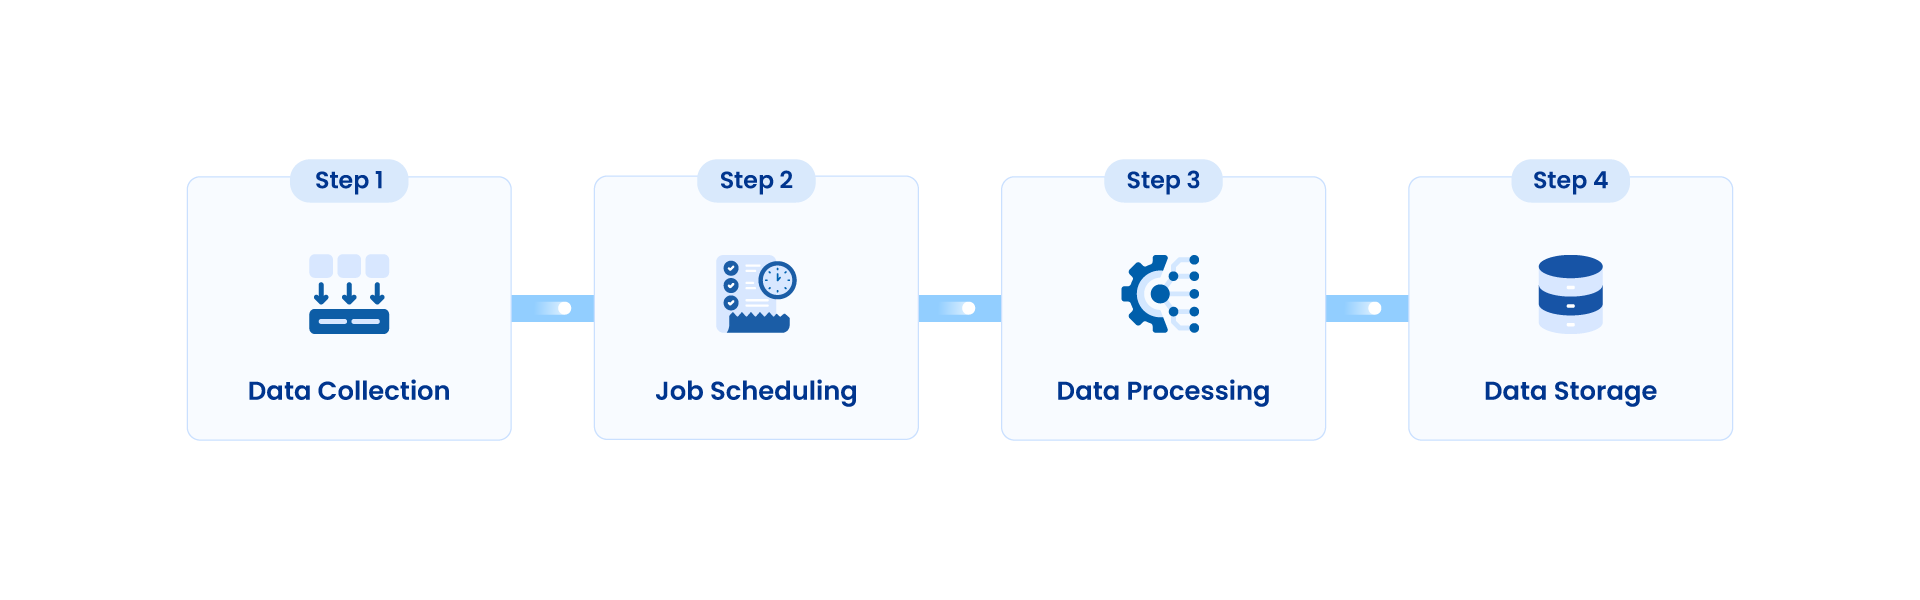
\includegraphics[width=1\textwidth]{images/batch-processing.png}
      \label{fig:batch-processing}
      {\footnotesize Fuente: Elaboración propia (datos simulados).}
\end{figure}

\textbf{Procesamiento en tiempo real (Streaming Processing):}

El procesamiento de flujo, también conocido como procesamiento en tiempo real, procesa continuamente los datos a medida que se reciben o generan. A diferencia del procesamiento por lotes, no existe el concepto de almacenar datos antes de procesarlos, lo que hace que esta técnica sea ideal para obtener resultados en tiempo real o procesar flujos de datos urgentes.

Su baja latencia y funcionamiento continuo caracterizan el procesamiento de flujo. Se usa comúnmente en aplicaciones que requieren que los datos se procesen en tiempo real para un análisis inmediato, como las plataformas de comercio financiero.

El procesamiento en tiempo real también es necesario para aplicaciones que deben evaluar y responder a eventos a medida que ocurren, como sistemas de detección de fraude, monitoreo de seguridad de red o dispositivos y dispositivos de Internet de las cosas (IoT).

\begin{figure}[H]
      \centering

      \caption{Procesamiento en tiempo real (Stream Processing)}
      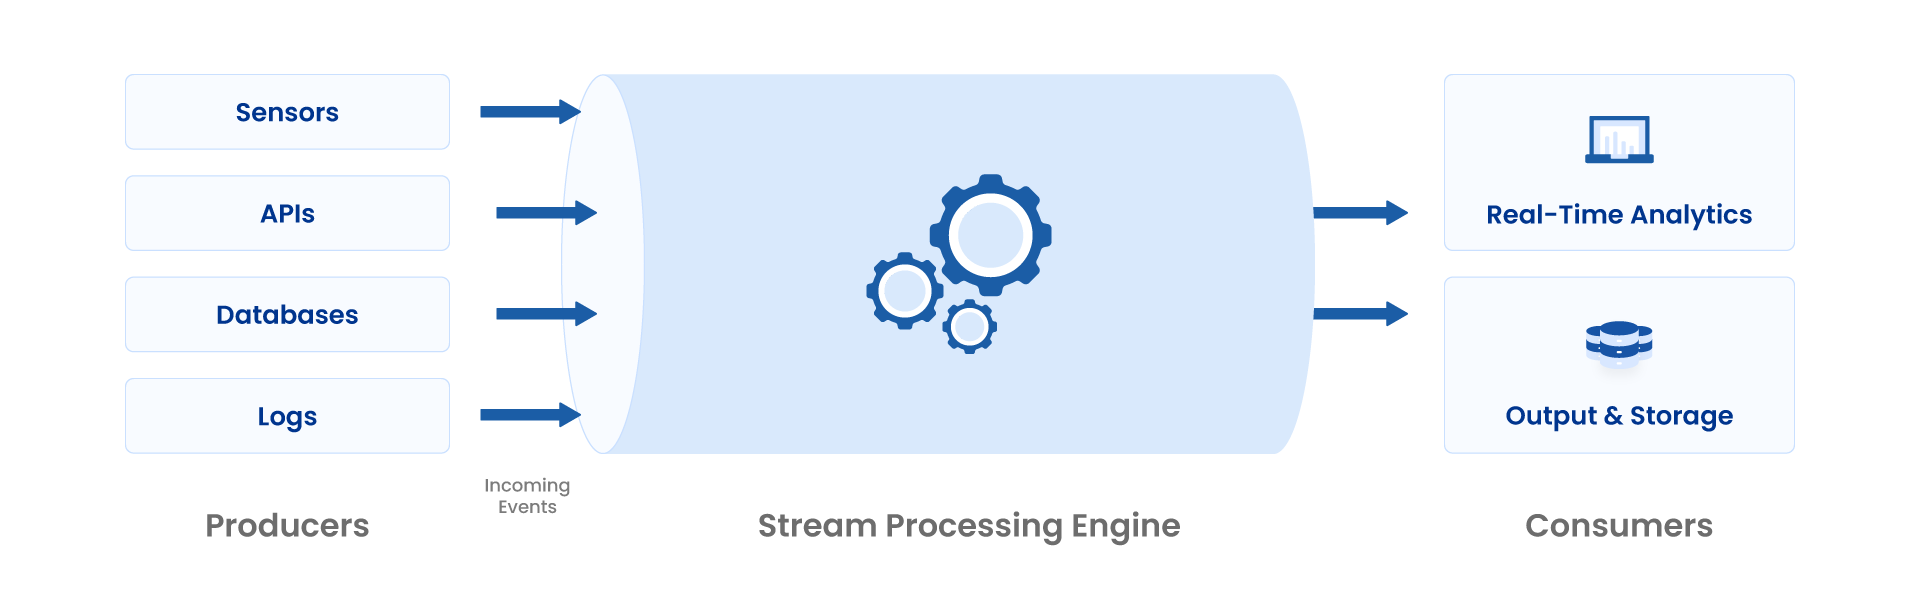
\includegraphics[width=1\textwidth]{images/stream-processing.png}
      \label{fig:stream-processing}
      {\footnotesize Fuente: Elaboración propia (datos simulados).}
\end{figure}


La comparativa se muestra en la \vref{fig:batch-vs-stream}.

\begin{figure}[H]
      \centering
      \caption{Comparativa entre procesamiento por lotes y en tiempo real}
      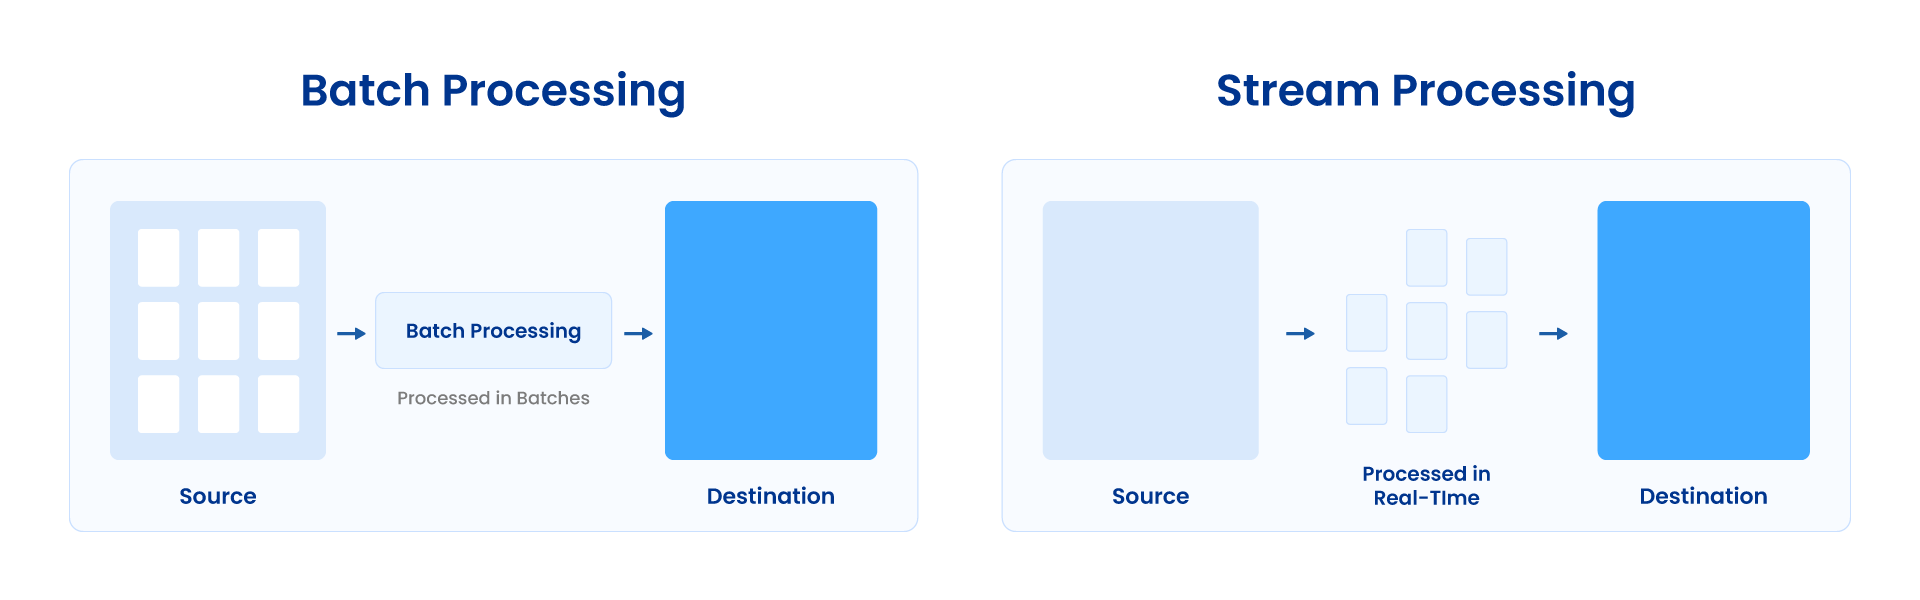
\includegraphics[width=1\textwidth]{images/batch-vs-stream.png}
      \label{fig:batch-vs-stream}
      {\footnotesize Fuente: Elaboración propia (datos simulados).}
\end{figure}

\subsubsection{Arquitecturas Big Data (Lambda, Kappa y Dataflow)}

\textbf{Arquitectura Lambda}

La arquitectura Lambda fue propuesta por Nathan Marz como un modelo para manejar grandes volúmenes de datos combinando el procesamiento por lotes (batch) y el procesamiento en tiempo real (streaming) en un sistema único \parencite{marz2015bigdata}. Esta arquitectura busca equilibrar precisión, latencia y tolerancia a fallos mediante tres capas principales: la capa batch que procesa todos los datos históricos, la capa speed que maneja los datos recientes en tiempo real, y la capa serving que combina ambos resultados para proporcionar consultas actualizadas \parencite{wikipedia2024lambda}.

La principal ventaja de Lambda es que permite reprocesar datos históricos y actualizar resultados de forma continua. Sin embargo, presenta una complejidad considerable al mantener dos caminos de procesamiento distintos, lo que puede duplicar el código y aumentar el costo de mantenimiento \parencite{marz2015bigdata}.

\begin{figure}[H]
      \centering
      \caption{Arquitectura Lambda: combinación de batch layer, speed layer y serving layer }
      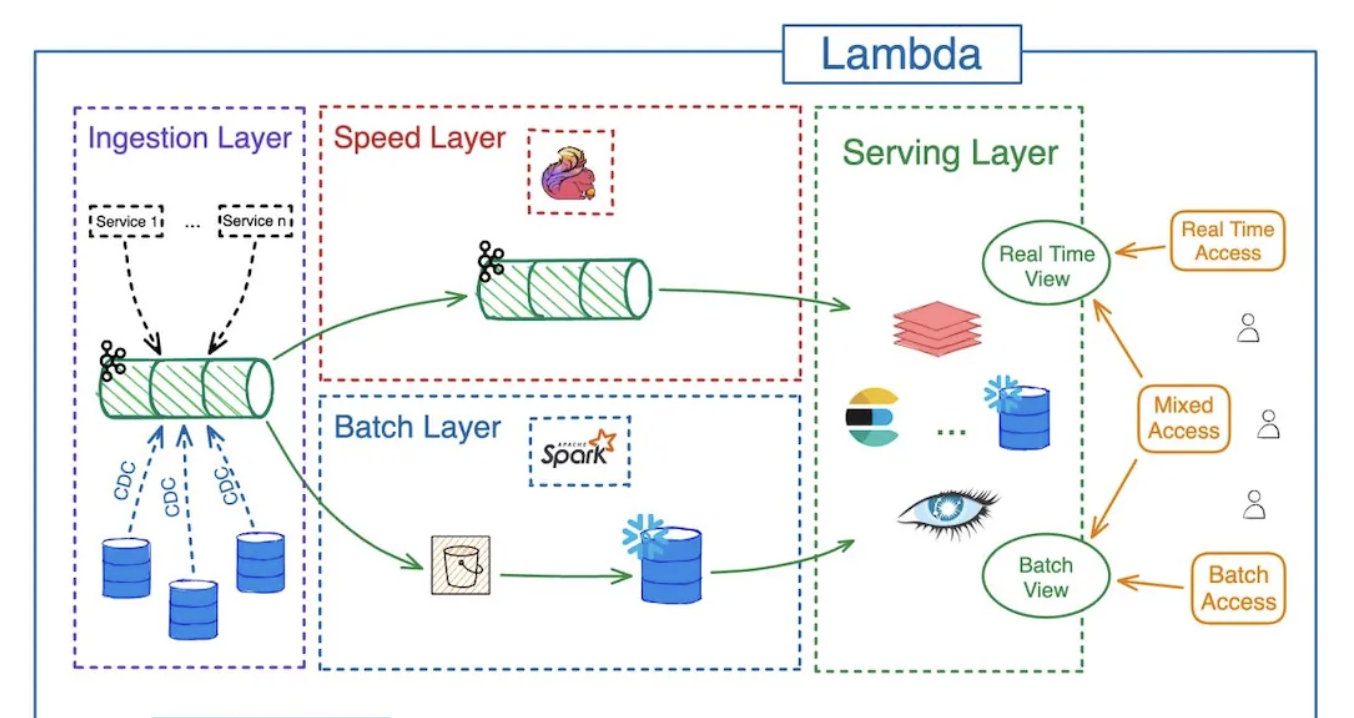
\includegraphics[width=1\textwidth]{images/lambda-architecture.png}
      \label{fig:lambda-architecture}
      {\footnotesize Fuente: https://medium.com/@FrankAdams7/what-is-the-difference-between-lambda-and-kappa-architectures-3806be298089}
\end{figure}

\textbf{Arquitectura Kappa}

La arquitectura Kappa fue propuesta por \textcite{kreps2014lambda}, cofundador de Apache Kafka, como una alternativa más simple a Lambda. Kappa elimina la capa de procesamiento por lotes y trata todos los datos como flujos de eventos. En lugar de mantener rutas separadas, los sistemas basados en Kappa procesan tanto los datos en tiempo real como los históricos desde un único flujo continuo \parencite{kreps2014lambda}.

Este enfoque reduce la complejidad operativa y permite re-procesar datos históricos volviendo a leer el log de eventos desde sistemas como Apache Kafka \parencite{hazelcast2025kappa}. Su simplicidad facilita la implementación de arquitecturas escalables para análisis y aprendizaje automático en tiempo real, aunque puede no ser tan eficiente como Lambda en tareas que requieren procesamiento intensivo sobre grandes volúmenes históricos \parencite{chaosgenius2025kappa}.

\begin{figure}[H]
      \centering
      \caption{Arquitectura Kappa: procesamiento continuo de flujos de eventos }
      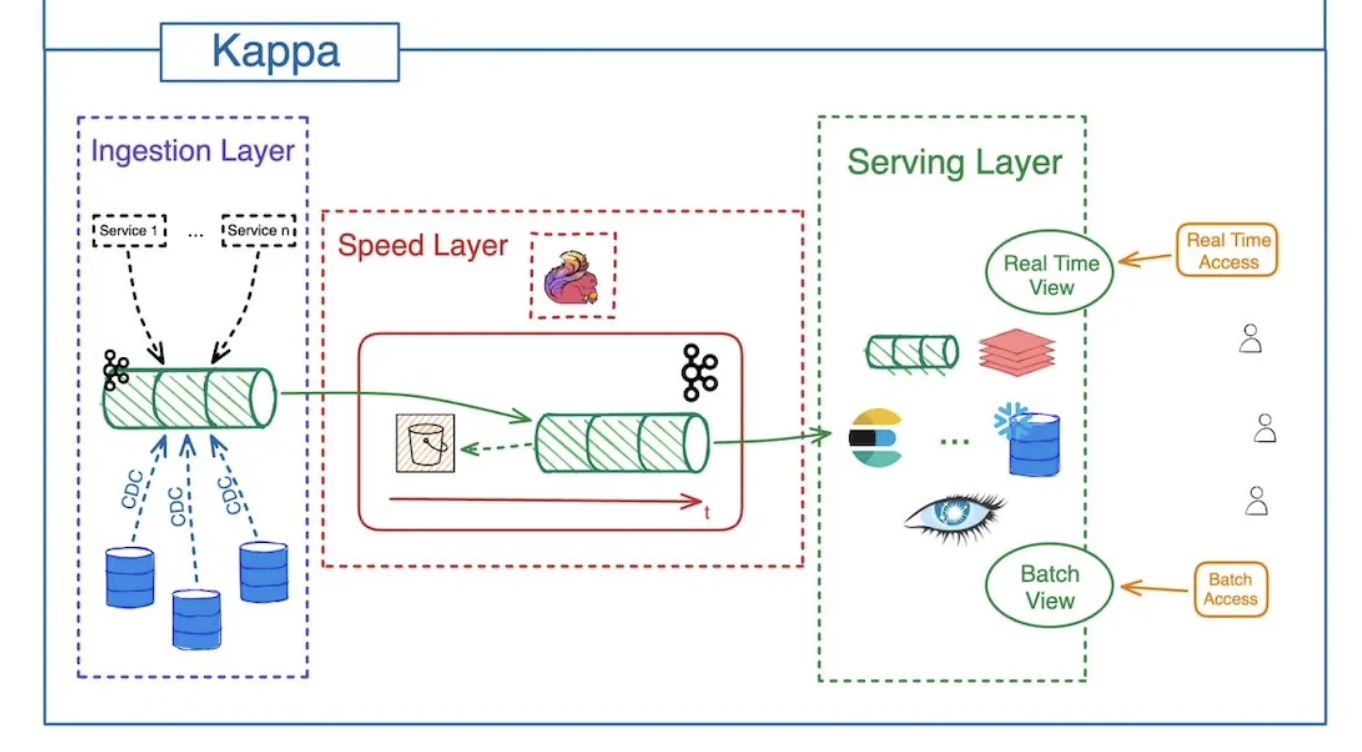
\includegraphics[width=1\textwidth]{images/kappa-architecture.png}
      \label{fig:kappa-architecture}
      {\footnotesize Fuente: https://medium.com/@FrankAdams7/what-is-the-difference-between-lambda-and-kappa-architectures-3806be298089}
\end{figure}
\textbf{Modelo Dataflow}

El modelo Dataflow, introducido por Google y formalizado por \textcite{akidau2015dataflow}, propone una unificación de los paradigmas batch y streaming bajo una misma abstracción de procesamiento. En este modelo, los datos se representan como colecciones (denominadas PCollections), sobre las cuales se aplican transformaciones que pueden ejecutarse tanto de manera continua como puntual \parencite{akidau2015dataflow}.

Dataflow incorpora conceptos avanzados como ventanas de tiempo (windows), triggers, procesamiento con estado (stateful processing) y semánticas de tiempo de evento (event time), lo que permite manejar tanto datos históricos como flujos en tiempo real \parencite{beam2024guide}. Su principal ventaja es que el mismo pipeline puede ser ejecutado sobre diferentes motores de ejecución (runners), como Apache Flink, Spark o Google Cloud Dataflow, favoreciendo la portabilidad y la flexibilidad.

Comparado con Lambda y Kappa, Dataflow puede considerarse una evolución conceptual: mantiene la capacidad de procesar datos históricos y en streaming, pero sin duplicar código ni requerir arquitecturas paralelas, lo que simplifica notablemente el mantenimiento de los sistemas de análisis.

\subsubsection{Comparativa técnica entre Lambda, Kappa y Dataflow}
Con el objetivo de analizar las diferencias prácticas entre las principales arquitecturas de procesamiento de datos a gran escala, se presenta a continuación una comparativa técnica entre las arquitecturas Lambda, Kappa y el modelo Dataflow.
La comparación se realiza atendiendo a criterios relevantes para sistemas de análisis en tiempo real, tales como la complejidad operativa, la duplicación de lógica de procesamiento, la capacidad de reprocesamiento, el manejo de eventos tardíos, la consistencia de resultados y los costos de mantenimiento.

\begin{table}[H]
      \centering
      \caption{Comparativa técnica entre arquitecturas Lambda, Kappa y Dataflow}
      \label{tab:lambda-kappa-dataflow}
      \begin{tabular}{@{}p{0.4\textwidth} p{0.2\textwidth} p{0.2\textwidth} p{0.2\textwidth}@{}}
            \toprule
            \textbf{Criterio}                           & \textbf{Lambda} & \textbf{Kappa} & \textbf{Dataflow} \\
            \midrule
            Complejidad operativa                       &
            Alta, requiere mantener múltiples capas     &
            Media, arquitectura más simple              &
            Baja, pipeline unificado                                                                           \\

            Duplicación de lógica                       &
            Sí, batch y speed layer separados           &
            No, una sola lógica                         &
            No, lógica única reutilizable                                                                      \\

            Reprocesamiento de datos                    &
            Completo, mediante batch layer              &
            Limitado, relectura del log                 &
            Completo, batch y streaming integrados                                                             \\

            Manejo de eventos tardíos                   &
            Limitado y dependiente de la implementación &
            Limitado                                    &
            Avanzado, mediante ventanas y watermarks                                                           \\

            Consistencia de resultados                  &
            Eventual, depende de la sincronización      &
            Alta en streaming                           &
            Alta y coherente entre batch y streaming                                                           \\

            Costos de mantenimiento                     &
            Altos, por duplicación de pipelines         &
            Medios                                      &
            Reducidos, menor complejidad                                                                       \\
            \bottomrule
      \end{tabular}
      \vspace{1em}
      {\footnotesize Fuente: Cuadro propio}
\end{table}

Del análisis comparativo se observa que la arquitectura Lambda, si bien ofrece una solución robusta para combinar procesamiento en tiempo real y por lotes, introduce una elevada complejidad operativa al requerir el mantenimiento de dos pipelines independientes. Esta duplicación de lógica incrementa los costos de desarrollo, operación y mantenimiento, y dificulta la evolución del sistema.

Por su parte, la arquitectura Kappa simplifica el diseño al unificar el procesamiento bajo un único flujo de eventos, apoyándose en la relectura del log para el reprocesamiento. Sin embargo, este enfoque presenta limitaciones cuando se requiere un reprocesamiento histórico intensivo o un manejo avanzado de eventos tardíos, especialmente en contextos donde la calidad y puntualidad de los datos no están garantizadas.

El modelo Dataflow se posiciona como una evolución conceptual de ambas arquitecturas, al proporcionar un marco unificado que integra de forma nativa el procesamiento batch y streaming. Su soporte explícito para ventanas temporales, triggers y watermarks permite gestionar eventos desordenados o tardíos sin comprometer la consistencia de los resultados. Asimismo, el uso de un único pipeline lógico reduce significativamente la complejidad operativa y los costos de mantenimiento, manteniendo coherencia entre los análisis en tiempo real y los reprocesamientos históricos.


\subsubsection{Procesamiento de datos}

\textbf{Apache Kafka (Google Pub/Sub)}

Apache Kafka es una plataforma distribuida de mensajería orientada a flujos de eventos (event streaming platform) desarrollada inicialmente por LinkedIn y actualmente mantenida por la Apache Software Foundation (2024a).

Permite la publicación, suscripción, almacenamiento y procesamiento de flujos de datos en tiempo real mediante un sistema basado en topics y brokers.

Su arquitectura distribuida garantiza alta disponibilidad, tolerancia a fallos y escalabilidad horizontal, lo que la convierte en un componente esencial para arquitecturas basadas en eventos.

\textbf{Kafka Connect}

Kafka Connect es un framework complementario a Apache Kafka diseñado para la integración de sistemas externos mediante conectores preconstruidos (connectors) (Apache Software Foundation, 2024b).

Permite mover datos de forma continua entre Kafka y otros sistemas ---como bases de datos, APIs o sistemas de archivos--- sin necesidad de programar procesos ETL complejos.

\textbf{Apache Beam (Google Dataflow)}

Apache Beam es un modelo de programación unificado para el procesamiento de datos en modo batch y streaming, inspirado en el modelo Dataflow propuesto por Google (Akidau et al., 2015; Apache Software Foundation, 2024c).

Beam abstrae las transformaciones y operaciones de los datos a través de un conjunto de primitivas comunes (PCollections, ParDo, GroupByKey, Windowing), lo que permite definir un pipeline único que puede ejecutarse en distintos motores distribuidos (runners), como Flink, Spark o Google Cloud Dataflow.

Su principal contribución al estado del arte radica en ofrecer una abstracción de alto nivel que combina el paradigma de streaming continuo con el de procesamiento por lotes, garantizando consistencia y portabilidad.

\textbf{Apache Flink (Google Dataflow)}

Apache Flink es un motor de procesamiento distribuido diseñado específicamente para análisis de flujos de datos en tiempo real (Apache Software Foundation, 2024d).

Flink implementa un modelo de ejecución streaming-first, con soporte nativo para stateful processing, event time, windowing y exactly-once semantics.

Su arquitectura permite ejecutar flujos de datos continuos con baja latencia y alta tolerancia a fallos, utilizando puntos de control (checkpoints) y estados consistentes

\subsubsection{Almacenamiento distribuido y Series Temporales}

\textbf{MongoDB (BigQuery)}

MongoDB es una base de datos NoSQL orientada a documentos, desarrollada para almacenar información semiestructurada en formato JSON o BSON \parencite{mongodb2024manual}.

A diferencia de las bases de datos relacionales tradicionales, MongoDB proporciona flexibilidad en el esquema, escalabilidad horizontal y una alta velocidad de lectura y escritura.

\textbf{Prometheus (Google Data Studio)}

Prometheus es una herramienta de monitorización y recopilación de métricas en tiempo real desarrollada originalmente por SoundCloud \parencite{prometheus2024doc}.

Su arquitectura se basa en un modelo pull, donde Prometheus recolecta periódicamente métricas de los sistemas instrumentados, almacenándolas en una base de datos de series temporales.

Permite definir alertas y reglas basadas en consultas expresadas en su propio lenguaje, PromQL.

\subsubsection{Visualización y alertas de datos en entornos analíticos}

\textbf{Grafana}

Grafana es una plataforma de visualización y análisis de métricas de código abierto que se integra con múltiples fuentes de datos, entre ellas Prometheus y MongoDB \parencite{grafana2024doc}.

Permite construir dashboards interactivos que facilitan la interpretación del comportamiento de los sistemas en tiempo real y la generación de alertas visuales.

\textbf{Scikit-learn (BigQuery ML)}

Scikit-learn es una biblioteca de aprendizaje automático (Machine Learning) desarrollada en Python, orientada al análisis estadístico y la construcción de modelos predictivos \parencite{pedregosa2011scikit}.

Proporciona una amplia gama de algoritmos para clasificación, regresión, clustering y reducción de dimensionalidad, además de herramientas para validación de modelos y feature engineering.

\subsubsection{Vacíos identificados}\label{vacuxedos-identificados}

Procesamiento en tiempo real o streaming con baja latencia: La mayoría de los estudios peruanos mencionados usan procesamiento batch o predicciones basadas en datos históricos. Tu pipeline Dataflow permitiría análisis continuo.

Uso del modelo Dataflow / Apache Beam: No encontré estudios que usen explícitamente Dataflow o Beam en Perú para monitoreo en salud pública.

Integración de múltiples flujos de datos: Muchos trabajos usan un tipo de dato (casos COVID, vacunación, etc.). Incorporar movilidad, capacidad hospitalaria, defunciones, etc., simultáneamente sería valioso.

Generación de alertas dinámicas basadas en umbrales configurables:
Estudios descriptivos o de predicción no siempre incluyen mecanismos de alerta automática en tiempo real.

Validación con latencia, tolerancia a fallos, ventana de tiempo avanzada (Windows / Triggers): No se evidencian trabajos que midan explícitamente latencia, manejo de eventos tardíos, watermarks, etc.

No obstante, ambas presentan desafíos: Lambda requiere mantener dos sistemas paralelos, lo que aumenta la complejidad del mantenimiento, mientras que Kappa puede tener dificultades para manejar procesamientos históricos.

\subsection{Trabajos Relevantes en Salud Pública y Big Data}

\begin{enumerate}

      \tightlist
      \item
            \emph{Modelo de una arquitectura big data para mejorar el análisis de datos abiertos del MINSA de casos COVID-19 en el Perú} --- \textcite{gomez2023modelo}.\\
            La tesis propone un modelo de arquitectura Big Data para optimizar el análisis de los datos abiertos del Ministerio de Salud (MINSA). Se evalúan eficiencia, calidad de registros, agilidad en generación de informes. Sin embargo, no queda claro que incluya procesamiento en streaming real ni ventanas de tiempo dinámicas, ni uso de modelos como Dataflow
      \item
            \emph{Solución de big data para el análisis de los datos abiertos de MINSA y CENARES para el monitoreo y control de la emergencia sanitaria COVID-19 bajo el ecosistema de Apache Hadoop y Microsoft Azure} --- \textcite{viteri2023solucion}.\\
            Esta tesis diseña una solución usando Hadoop + servicios en la nube Azure, para monitoreo y control de emergencia. Se orienta hacia análisis de datos abiertos, dashboards, etc. Pero nuevamente, se centra más en procesamiento por lotes, o en análisis no necesariamente en streaming con baja latencia.
      \item
            \emph{Implementación de una plataforma Big Data para el estudio de casos de anemia en América Latina} --- \textcite{bustamante2019implementacion}, Universidad Nacional del Altiplano.\\
            Plataforma que recolecta datos, los almacena (Hadoop, HDFS, etc.), usa herramientas de Big Data para consultas, minería de datos y visualización. Tiene algunos componentes de ingestión continua (por ejemplo, Flume para streaming desde API externas), pero no está específicamente orientada al modelo Dataflow ni al análisis epidemiológico en tiempo real
      \item
            \emph{Big data y toma de decisiones en el sector público peruano} --- \textcite{guillen2025big}.\\
            Este artículo analiza los beneficios y barreras del uso de Big Data en la administración pública del Perú. No se enfoca específicamente en salud ni en procesamiento en streaming, pero aporta contexto institucional, desafíos técnicos (infraestructura, talento humano) y normativos. Esto es útil para entender el entorno en el que tu TFM se desarrollará
      \item
            \emph{Transformación digital: Perú valida interoperabilidad de historias clínicas electrónicas} --- \textcite{ops2025interoperabilidad}.\\ Se trata de una iniciativa reciente que busca interoperabilidad en los registros clínicos electrónicos. Esto aporta al contexto tecnológico, interoperabilidad y digitalización de datos en salud en Perú, lo cual será relevante para integraciones de datos en tu pipeline.
      \item
            La arquitectura Lambda, propuesta por Nathan Marz, combina dos vías de procesamiento complementarias: una vía por lotes (batch layer) para procesar datos históricos completos y otra vía de velocidad (speed layer) para procesar datos recientes en tiempo real, junto con una capa de consulta (serving layer) que unifica ambas salidas
\end{enumerate}

\subsection{Propuesta}\label{propuesta}

La propuesta que está enfocada a usar el modelo Dataflow, puede aportar
lo siguiente:

\begin{itemize}
      \tightlist
      \item
            Arquitectura unificada que soporte tanto streaming como batch, lo que permite mayor flexibilidad y adaptabilidad.
      \item
            Cálculo de métricas epidemiológicas casi en tiempo real, apoyando decisiones sanitarias ágiles.
      \item
            Manejo de ventanas de tiempo, triggers, watermarks, para tratar datos con retrasos, lo que mejora la robustez del análisis.
      \item
            Generación de alertas y dashboards que reflejen dinámicamente la situación de una pandemia simulada en Perú, lo que puede servir como piloto para entornos reales.
      \item
            Comparación con trabajos previos peruanos para demostrar mejoras en latencia, integración de flujos, precisión, etc.
\end{itemize}

\subsection{Conclusiones}\label{conclusiones-estado-arte}

El análisis del estado del arte permite identificar que el procesamiento en tiempo real se ha consolidado como una de las tendencias más importantes dentro del ámbito del Big Data. Tecnologías como Apache Kafka, Apache Beam, Google Cloud Dataflow y Apache Flink ofrecen soluciones maduras para manejar grandes volúmenes de información con baja latencia y alta disponibilidad.

Los modelos de procesamiento ---en particular el modelo Dataflow--- proporcionan un marco conceptual robusto para integrar tanto procesamiento por lotes (\emph{batch}) como en flujo (\emph{streaming}), logrando sistemas híbridos capaces de adaptarse a distintos tipos de datos y escenarios. Asimismo, las arquitecturas Lambda y Kappa representan enfoques complementarios que han evolucionado para atender diferentes necesidades: la primera prioriza la precisión mediante la coexistencia de capas batch y speed, mientras que la segunda busca simplicidad y unificación total bajo el paradigma de flujo continuo.

Por otra parte, las herramientas de almacenamiento (BigQuery, Elasticsearch, Cassandra), visualización (Grafana, Kibana, Tableau) y alertas o predicción (Prometheus, TensorFlow, Scikit-learn) han permitido que los sistemas de análisis de datos sean más interactivos y accesibles para la toma de decisiones. Estas tecnologías habilitan un ecosistema integral que va desde la captura hasta la interpretación de datos, consolidando el ciclo completo de inteligencia operativa.

En el contexto peruano, se observa que, aunque existen avances en la gestión y publicación de datos epidemiológicos (por ejemplo, las plataformas del MINSA y del Instituto Nacional de Salud), la mayoría de las soluciones implementadas se basan en procesamiento por lotes, lo que limita su capacidad para generar alertas o proyecciones en tiempo real. Esta brecha tecnológica representa una oportunidad para explorar soluciones basadas en arquitecturas de streaming que optimicen la velocidad de análisis y respuesta.

Por tanto, se concluye que el desarrollo de un pipeline de procesamiento en tiempo real basado en el modelo Dataflow, y apoyado en herramientas de Big Data, visualización y predicción, constituye una contribución innovadora y necesaria para el tratamiento de datos epidemiológicos en el Perú.\\
Este enfoque permitirá simular y analizar la evolución de la pandemia COVID-19 con mayor precisión temporal, escalabilidad y capacidad de adaptación, contribuyendo a mejorar la gestión de información crítica en contextos de emergencia sanitaria.

\clearpage
\section{Objetivos concretos y metodología de trabajo}\label{objetivos-concretos-y-metodologuxeda-de-trabajo}

\subsection{Objetivo general}\label{objetivo-general}

Desarrollar e implementar una arquitectura analítica avanzada para la simulación, predicción y comprensión de tendencias epidemiológicas relacionadas con la COVID-19 en Perú, utilizando procesamiento de datos en tiempo real y por lotes basado en el modelo Dataflow, técnicas de machine learning y herramientas de visualización interactiva, con el fin de ofrecer una solución robusta, segura y orientada a la toma de decisiones fundamentadas en datos.

\subsection{Objetivos específicos}\label{objetivos-especuxedficos}

\begin{itemize}
      \tightlist
      \item
            Analizar los requisitos funcionales, técnicos y epidemiológicos necesarios para construir una arquitectura de procesamiento de datos en tiempo real y en lotes basada en flujos de evento
      \item
            Diseñar un flujo de procesamiento utilizando el modelos Dataflow que permita integrar, transformar, almacenar y gestionar datos epidemiológicos en tiempo real y por lotes de manera eficiente y escalable.
      \item
            Implementar el procesamiento de datos en streaming y batch utilizando Apache Beam y el modelo Dataflow, aplicando transformaciones, ventanas temporales, agregaciones y cálculos analíticos relevantes.
      \item
            Implementar modelos analíticos y predictivos que permitan identificar tendencias, comportamientos inusuales y posibles escenarios futuros en los datos epidemiológicos.
      \item
            Diseñar e implementar dashboards de visualización interactiva que permitan interpretar indicadores epidemiológicos en tiempo real, facilitando la exploración y seguimiento de los datos.
      \item
            Evaluar el desempeño del modelo analítico mediante métricas cuantitativas que permitan verificar la precisión, latencia y utilidad práctica del sistema desarrollado
\end{itemize}

\subsection{Metodología del trabajo}\label{metodologuxeda-del-trabajo}

En este Trabajo Fin de Máster se adopta una metodología híbrida compuesta por:

\begin{itemize}
      \tightlist
      \item
            \textbf{CRISP-DM (Cross Industry Standard Process for Data Mining)}, que proporciona la estructura principal para el análisis, preparación de datos, diseño del sistema y evaluación del funcionamiento.
      \item
            \textbf{Kanban ligero}, que permite gestionar de manera flexible y visual las tareas del proyecto, manteniendo un flujo constante
\end{itemize}

Este enfoque híbrido garantiza:

\begin{itemize}
      \tightlist
      \item
            Rigor analítico y claridad metodológica (CRISP-DM).
      \item
            Organización eficiente del desarrollo, priorización y control del avance (Kanban).
      \item
            Adaptabilidad para iterar, corregir y mejorar durante todo el proceso.
\end{itemize}

\subsubsection{Aplicación del modelo CRISP-DM}

\textbf{Comprensión del negocio}

En esta primera fase se define el problema principal que aborda el TFM: la necesidad de diseñar una arquitectura capaz de procesar datos tanto en tiempo real como en modo batch mediante flujos de eventos. Se estudia el contexto donde esta necesidad cobra relevancia y se establecen los requisitos funcionales y no funcionales que la solución debe cumplir, incluyendo aspectos de latencia, consistencia y tolerancia a fallos.

como:

\begin{itemize}
      \tightlist
      \item
            Análisis de casos de uso similares en entornos de salud pública, IoT y analítica en streaming.
      \item
            Definición de los objetivos generales y específicos del TFM.
      \item
            Identificación de requisitos funcionales (procesamiento continuo, almacenamiento en sinks, visualización en dashboards) y no funcionales (latencia mínima, throughput, resiliencia).
      \item
            Establecimiento de los criterios de éxito: correcta operación del pipeline, rendimiento aceptable, consistencia entre batch y streaming y reproducibilidad de la solución.
\end{itemize}

\subsubsection{\texorpdfstring{Comprensión de los datos}{Comprensión de los datos}}\label{comprensiuxf3n-de-los-datos}

A continuación, se analiza la naturaleza de los datos que alimentan el sistema, simulados como provenientes de fuentes reales. Se examinan sus características estructurales, su comportamiento temporal, su calidad y las limitaciones asociadas a su uso. Este análisis permite identificar los ajustes necesarios antes de integrarlos en los flujos de procesamiento.

\begin{itemize}
      \tightlist
      \item
            Identificación del flujo de datos simulado o real.
      \item
            Análisis de la estructura de los mensajes y campos relevantes.
      \item
            Estudio de la tasa de llegada de eventos (event time vs. processing time).
      \item
            Evaluación de la calidad de los datos: registros incompletos, duplicados, anomalías temporales.
      \item
            Identificación de limitaciones derivadas de formatos y disponibilidad.
\end{itemize}

\subsubsection{\texorpdfstring{Preparación de los datos}{Preparación de los datos}}\label{preparaciuxf3n-de-los-datos}

En esta fase se lleva a cabo la limpieza, estandarización y normalización de los datos. Se definen los esquemas de ingestión y se estructuran los mensajes que serán enviados a los flujos de procesamiento. Asimismo, se preparan los timestamps, se ajustan los formatos y se generan las estructuras de datos necesarias tanto para la ingesta en streaming como para la ejecución en modo batch.

\begin{itemize}
      \tightlist
      \item
            Limpieza y estandarización de valores.
      \item
            Transformaciones iniciales y normalización.
      \item
            Definición de esquemas para la ingestión en Kafka.
      \item
            Diseño de los tópicos, particiones y claves de mensajes.
      \item
            Configuración de criterios temporales: timestamps, ventanas de tiempo y manejo del retraso en la llegada de eventos.
      \item
            Preparación de la estructura del dataset para el modo batch.
\end{itemize}

\subsubsection{\texorpdfstring{Modelado}{Modelado}}\label{modelado}

El modelado corresponde al diseño de la arquitectura basada en el modelo Dataflow. Aquí se define el flujo completo del sistema: ingestión, procesamiento y almacenamiento. Se especifican las transformaciones a aplicar sobre los datos, el manejo de ventanas de tiempo, triggers y watermarks, así como la integración con herramientas de almacenamiento y visualización. Esta fase establece la estructura técnica que luego será implementada.

\begin{itemize}
      \tightlist
      \item
            Diseño conceptual del pipeline.
      \item
            Definición de flujos
      \item
            Selección de tecnologías: Apache Kafka, Apache Beam, Apache Flink, MongoDB y Grafana.
\end{itemize}

\subsubsection{\texorpdfstring{Evaluación}{Evaluación}}\label{evaluaciuxf3n}

Una vez implementado el sistema, se evalúa su funcionamiento mediante pruebas de rendimiento y consistencia. Se analizan métricas como latencia, capacidad de procesamiento, estabilidad bajo diferentes cargas y comportamiento ante fallos o retrasos en la llegada de eventos. Los resultados obtenidos permiten valorar el grado de cumplimiento de los requisitos definidos al inicio del proyecto.

\begin{itemize}
      \tightlist
      \item
            Latencia end-to-end del pipeline.
      \item
            Throughput bajo diferentes tasas de llegada de datos.
      \item
            Tolerancia a fallos del broker y del motor de ejecución.
      \item
            Consistencia entre batch y streaming.
      \item
            Escalabilidad ante incrementos de carga.
      \item
            Las pruebas se diseñan para representar escenarios realistas de operación
\end{itemize}

\subsubsection{\texorpdfstring{Despliegue}{Despliegue}}\label{despliegue}

Finalmente, se consolida la solución desarrollada, documentando la arquitectura final y configurando un entorno reproducible para futuras ejecuciones o ampliaciones. Esta fase incluye la integración de herramientas de visualización y la generación de evidencias que demuestran el funcionamiento del sistema.

\begin{itemize}
      \tightlist
      \item
            Documentación de la arquitectura final.
      \item
            Registro de configuraciones empleadas en Kafka, Beam/Flink, almacenamiento y visualización.
      \item
            Generación de scripts o contenedores para facilitar la replicación del sistema.
\end{itemize}

\subsection{Gestión del trabajo mediante Kanban}

El avance del proyecto se organiza mediante un tablero Kanban dividido en las columnas To Do, In Progress, In Review y Done. Este enfoque permite gestionar de manera visual y flexible las tareas del TFM, acomodar iteraciones según los resultados y asegurar un progreso continuo. Kanban proporciona un marco adecuado para un trabajo individual que requiere experimentación y ajustes frecuentes, como es el caso de la construcción de pipelines de datos.

\clearpage
\section{Marco normativo}\label{marco-normativo}

El presente Trabajo Fin de Máster se ajusta al marco jurídico vigente en materia de privacidad y protección de datos personales, especialmente en lo relativo al tratamiento de información que pudiera identificar directa o indirectamente a personas físicas. En particular, resultan de referencia el Reglamento (UE) 2016/679, General de Protección de Datos (RGPD), y la Ley Orgánica 3/2018, de Protección de Datos Personales y garantía de los derechos digitales (LOPDGDD), aplicables en el contexto académico y profesional.

Estas normativas establecen los principios y obligaciones que deben cumplirse cuando se tratan datos personales, como la licitud del tratamiento, la minimización de datos, la integridad y confidencialidad, así como la responsabilidad proactiva del responsable del tratamiento.

En el contexto del presente TFM, los datos empleados para la construcción y evaluación de la arquitectura de procesamiento en tiempo real y por lotes no contienen información personal identificable. El proyecto utiliza datos anonimizados, simulados y datos públicos provistos por el gobierno y fuentes publicas , generados exclusivamente con fines experimentales para alimentar los pipelines de ingestión, transformación y análisis. Dado que la anonimización es irreversible y no existe posibilidad de vincular los datos a individuos concretos, estos no entran en la categoría de datos personales según la definición del artículo 4 del RGPD.

Por tanto, el tratamiento realizado en este trabajo no activa las obligaciones del RGPD ni de la LOPDGDD, al no existir un riesgo para los derechos y libertades de personas físicas. Aun así, se ha procedido a revisar las disposiciones normativas y la Guía sobre privacidad y protección de datos personales (Anexo N.º 1) proporcionada por la institución académica, confirmando que el uso de datos anonimizados elimina la necesidad de aplicar medidas adicionales de protección propias del tratamiento de datos personales.

El proyecto se ha desarrollado en entornos controlados, utilizando sistemas locales y aislados (p. ej., contenedores Docker con Kafka, Apache Beam, Flink y MongoDB), sin exponer información en repositorios públicos ni transmitir datos a terceros. manteniendo siempre los principios de seguridad y minimización de datos recomendados en la normativa.

En conclusión, el desarrollo del TFM se considera plenamente conforme con la normativa vigente en protección de datos, dado que no se tratan datos personales en ninguno de los procesos realizados, y las medidas adoptadas garantizan la inexistencia de riesgos para la privacidad.

La Ley de Protección de Datos Personales en Perú es la Ley N° 29733, que protege el derecho fundamental a la privacidad de los ciudadanos, regulando el tratamiento (recopilación, uso, almacenamiento) de datos personales para asegurar su adecuado manejo por entidades públicas y privadas, garantizando derechos como el acceso.

fuentes de dataset:

\begin{itemize}
      \tightlist
      \item \url{https://www.datosabiertos.gob.pe/dataset/fallecidos-hospitalizados-y-vacunados-por-covid-19/resource/ad49459e-7ef9-4a6f-bb4d}
      \item \url{https://www.datosabiertos.gob.pe/dataset/informaci\%C3\%B3n-de-fallecidos-del-sistema-inform\%C3\%A1tico-nacional-de-defunciones-sinadef-ministerio}
      \item \url{https://www.datosabiertos.gob.pe/dataset/informaci\%C3\%B3n-de-fallecidos-del-sistema-inform\%C3\%A1tico-nacional-de-defunciones-sinadef-ministerio}
\end{itemize}

Con el propósito de minimizar riesgos, se aplican medidas de protección
y buenas prácticas tales como:

\begin{itemize}
      \tightlist
      \item Uso de los datos en un entorno local o aislado.
      \item Uso restringido únicamente al autor del TFM.
      \item Eliminación del campo UUID del dataset pm26Sep2023 tras el procesamiento
\end{itemize}

\clearpage
\section{Desarrollo específico de la contribución}\label{desarrollo-especuxedfico-de-la-contribuciuxf3n}

\subsection{\texorpdfstring{Visión general de la contribución}{Visión general de la contribución}}\label{visiuxf3n-general-de-la-contribuciuxf3n}

El presente Trabajo Fin de Máster propone el diseño, implementación y evaluación de una arquitectura unificada de procesamiento de datos en streaming y batch basada en flujos de eventos y en el modelo Dataflow, aplicada a la simulación y análisis de datos epidemiológicos relacionados con la pandemia de la COVID-19 en el Perú. La contribución abarca cuatro ejes principales:


\begin{enumerate}
    \item \textbf{Pipeline de procesamiento unificado}: Un pipeline implementado en Apache Beam que procesa tanto datos históricos (batch) como datos en tiempo real (streaming) utilizando el mismo código base, con ingesta a través de Apache Kafka y almacenamiento en colecciones Time-Series de MongoDB.
    \item \textbf{Capa analítica y predictiva}: Modelos de análisis descriptivo, detección de anomalías y predicción a corto plazo que se integran dentro del pipeline (en línea) y sobre los datos almacenados (fuera de línea), generando métricas epidemiológicas y escenarios futuros.
    \item \textbf{Visualización interactiva}: Dashboards que presentan métricas en tiempo real, series temporales, distribuciones geográficas y predicciones, permitiendo a los usuarios explorar los datos y tomar decisiones informadas.
    \item \textbf{Sistema de alertas y monitorización}: Mecanismo automatizado de detección de eventos críticos con notificaciones por múltiples canales, tanto para indicadores epidemiológicos como para el estado operativo de la infraestructura.
\end{enumerate}

\begin{figure}[H]
\centering
\begin{tikzpicture}[
    node distance=0.5cm,
    layer/.style={rectangle, draw, rounded corners, minimum width=3cm, minimum height=1.2cm, align=center, fill=#1, font=\small},
    arrow/.style={->, thick}
]
    \node[layer=green!20] (ingest) {Ingesta\\Kafka + CSV};
    \node[layer=orange!20, right=1.5cm of ingest] (pipeline) {Pipeline Beam\\Transforms + DLQ};
    \node[layer=blue!15, right=1.5cm of pipeline] (store) {Almacenamiento\\MongoDB Time-Series};
    \node[layer=yellow!30, right=1.5cm of store] (analytics) {Analítica\\Modelos + Métricas};
    \node[layer=red!15, below=1.5cm of analytics] (alerts) {Alertas\\Detección + Notificación};
    \node[layer=purple!15, below=1.5cm of store] (viz) {Visualización\\Dashboards + Reportes};

    \draw[arrow] (ingest) -- (pipeline);
    \draw[arrow] (pipeline) -- (store);
    \draw[arrow] (store) -- (analytics);
    \draw[arrow] (analytics) -- (alerts);
    \draw[arrow] (store) -- (viz);
    \draw[arrow] (alerts) -- (viz);
\end{tikzpicture}
\caption{Visión general de las capas del sistema}
\end{figure}

El sistema procesa dos tipos de datos epidemiológicos provenientes de fuentes oficiales:

\begin{table}[H]
\centering
\caption{Datasets procesados por el sistema}
\begin{tabular}{@{}llrl@{}}
\toprule
\textbf{Dataset} & \textbf{Schema} & \textbf{Registros} & \textbf{Variables clave} \\
\midrule
Casos & \texttt{cases} & 1,048,575 & fecha\_muestra, edad, sexo, resultado, ubicación \\
Fallecimientos & \texttt{demises} & 220,918 & fecha\_fallecimiento, edad, sexo, clasificación, ubicación \\
\bottomrule
\end{tabular}
\end{table}

La arquitectura sigue el patrón Kappa, donde todos los datos fluyen a través de Apache Kafka como bus de eventos central, simplificando el diseño al eliminar la necesidad de mantener dos pipelines separados para batch y streaming.

\subsection{\texorpdfstring{Análisis de requisitos del sistema}{Análisis de requisitos del sistema}}\label{anuxe1lisis-de-requisitos-del-sistema}

El analisis de requisitos que debe cumplir el sistema propuesto, tanto desde una perspectiva funcional como no funcional y epidemiológica. Estos requisitos se han definido a partir del análisis del dominio del problema, las características de los datos epidemiológicos y los objetivos del procesamiento en tiempo real y por lotes, garantizando que la arquitectura diseñada sea adecuada para la monitorización y análisis de la evolución de la enfermedad.

\subsection{\texorpdfstring{Requisitos
            funcionales}{Requisitos funcionales}}\label{requisitos-funcionales}

El sistema debe ser capaz de ingerir datos epidemiológicos en tiempo real procedentes de fuentes de mensajería como Apache Kafka, permitiendo la incorporación continua de nuevos eventos conforme se generan. Esta capacidad resulta esencial para reflejar de manera actualizada la evolución de los indicadores epidemiológicos y posibilitar la detección temprana de cambios relevantes.

Asimismo, el sistema debe soportar procesamiento tanto en modalidad en tiempo real como en lotes, de forma que sea posible analizar datos históricos mediante procesos por lotes y, simultáneamente, tratar los eventos entrantes en tiempo real. Esta dualidad permite reutilizar la misma lógica de transformación y validación en ambos contextos, alineándose con el modelo Dataflow.

Otro requisito fundamental es la generación de métricas epidemiológicas, tales como recuentos de casos, tasas de incidencia o indicadores derivados, a partir de los datos procesados. Estas métricas constituyen la base para el análisis posterior y para la toma de decisiones informadas.

El sistema debe permitir también la predicción de tendencias, facilitando el análisis de la evolución temporal de los datos y la identificación de patrones que puedan anticipar incrementos o descensos significativos en la incidencia de la enfermedad.

Finalmente, se requiere la visualización de la información y la generación de alertas, de manera que los resultados del procesamiento puedan ser consultados de forma clara e intuitiva mediante herramientas de visualización, así como la emisión de alertas cuando se superen determinados umbrales predefinidos.
Los requisitos funcionales del sistema son:

\begin{table}[H]
\centering
\caption{Requisitos Funcionales del Sistema}
\begin{tabular}{@{}p{3cm}p{10cm}@{}}
\toprule
\textbf{ID} & \textbf{Descripción} \\
\midrule
RF-01 & El sistema debe ingestar datos desde archivos CSV y enviarlos a Apache Kafka \\
RF-02 & El sistema debe consumir mensajes de Kafka en tiempo real \\
RF-03 & El sistema debe normalizar los datos (limpieza de nulos, tipos) \\
RF-04 & El sistema debe validar los registros contra esquemas JSON definidos \\
RF-05 & El sistema debe asignar timestamps para procesamiento temporal \\
RF-06 & El sistema debe aplicar ventanas temporales a los datos \\
RF-07 & El sistema debe agregar metadata de procesamiento \\
RF-08 & El sistema debe agrupar registros en batches para escritura eficiente \\
RF-09 & El sistema debe almacenar los datos en MongoDB \\
RF-10 & El sistema debe manejar errores mediante Dead Letter Queue \\
RF-11 & El sistema debe soportar ejecución en modo streaming y batch \\
\bottomrule
\end{tabular}
\end{table}

\subsection{\texorpdfstring{Requisitos no funcionales}{Requisitos no funcionales}}\label{requisitos-no-funcionales}

Desde el punto de vista no funcional, el sistema debe garantizar escalabilidad, permitiendo incrementar su capacidad de procesamiento conforme aumente el volumen de datos sin necesidad de rediseñar la arquitectura. Este aspecto es especialmente relevante en escenarios epidemiológicos, donde el número de eventos puede variar de forma significativa.

La arquitectura debe ofrecer baja latencia, de modo que exista un retardo mínimo entre la llegada de un evento y su disponibilidad para el análisis y la visualización. Esto resulta crítico en contextos de monitorización en tiempo real.

Asimismo, el sistema debe ser tolerante a fallos, asegurando la continuidad del procesamiento incluso ante errores en componentes individuales, como caídas temporales de servicios o recepción de datos inválidos.

En términos de seguridad, se requiere implementar mecanismos de control de acceso y protección de la información, garantizando que solo los usuarios y servicios autorizados puedan acceder a los datos y resultados, especialmente considerando la sensibilidad de la información sanitaria.

Por último, el pipeline debe ser reproducible, permitiendo ejecutar nuevamente los procesos sobre los mismos datos y obtener resultados consistentes. Este requisito es clave tanto para la validación académica del trabajo como para la trazabilidad de los análisis realizados.

\subsection{\texorpdfstring{Requisitos epidemiológicos}{Requisitos epidemiológicos}}\label{requisitos-epidemioluxf3gicos}

El sistema debe contemplar distintos tipos de eventos epidemiológicos, tales como casos confirmados, hospitalizaciones y fallecimientos, los cuales presentan características y necesidades de análisis diferenciadas.

Asimismo, es necesario definir ventanas temporales relevantes para el análisis, como ventanas diarias, semanales o móviles, que permitan estudiar la evolución de la enfermedad en distintos horizontes temporales.

Entre los resultados esperados se incluyen indicadores epidemiológicos clave, como el número reproductivo efectivo o la incidencia acumulada, los cuales requieren un tratamiento específico de los datos y un cálculo consistente a lo largo del tiempo.

Finalmente, se debe considerar la frecuencia y granularidad de los datos, garantizando que el sistema pueda manejar información a nivel individual o agregado, según el caso, y adaptarse a diferentes ritmos de actualización sin perder consistencia ni precisión en los resultados.

\subsection{\texorpdfstring{Diseño de la arquitectura basada en el modelo Dataflow}{Diseño de la arquitectura basada en el modelo Dataflow}}\label{diseuxf1o-de-la-arquitectura-basada-en-el-modelo-dataflow}

\subsubsection{Principios del modelo Dataflow aplicados}\label{principios-del-modelo-dataflow-aplicados}

El diseño de la arquitectura propuesta se fundamenta en el modelo Dataflow, el cual plantea un enfoque unificado para el procesamiento de datos en streaming y batch. A diferencia de las arquitecturas tradicionales, el modelo Dataflow permite tratar ambos tipos de procesamiento bajo un mismo paradigma, simplificando la complejidad el sistema y mejorando su mantenibilidad.

\begin{itemize}
      \tightlist
      \item
            Eventos como entidad central: cada dato epidemiológico se modela como un evento que contiene información asociada al tiempo de ocurrencia (event time), lo que permite análisis temporales más precisos.
      \item
            Procesamiento unificado: el mismo pipeline lógico es utilizado tanto para datos en tiempo real como para datos históricos, diferenciándose únicamente en el modelo de ejecución.
      \item
            Separación entre lógica y ejecución: el modelo Dataflow desacopla el motor de ejecución, permitiendo su despliegue en distintos entornos sin modificar la lógica del procesamiento.
      \item
            Windows, triggers y watermarks: posibilitan la agregación de datos en intervalos relevantes para el análisis epidemiológico.
      \item
            Gestión explícita del tiempo: el uso de event time, processing time y watermarks permite manejar eventos tardíos y desordenados de forma controlada.
\end{itemize}

\subsubsection{Arquitectura general del sistema}\label{arquitectura-general-del-sistema}

La arquitectura propuesta sigue un enfoque modular y desacoplado, organizado en capas funcionales que interactúan a través de flujos de eventos. Esta organización facilita la usabilidad, la tolerancia a fallos y la evolución del sistema.

\begin{itemize}
      \tightlist
      \item
            Diagrama de arquitectura.
      \item
            Componentes:
            \begin{itemize}
                  \tightlist
                  \item
                        Recolección de datos: datos extraídos de fuentes públicas, generadas y/o simuladas para reproducir patrones temporales y variabilidad realista.
                  \item
                        Sistema de ingesta de eventos: utiliza la plataforma de \emph{event streaming Kafka }para recibir y distribuir los eventos de forma continua y confiable.
                  \item
                        Pipeline de procesamiento: implementa la lógica de transformación, agregación y análisis de los datos, siguiendo el modelo Dataflow.
                  \item
                        Motor de ejecución: ejecuta el pipeline en modo \emph{streaming} o \emph{batch, }garantizando paralelismo, tolerancia a fallos y escalabilidad automática.
                  \item
                        Sistemas de almacenamiento: almacena tanto datos crudos como datos procesados para análisis en tiempo real e histórico.
                  \item
                        Capa de visualización y alertas: permite la exploración interactiva de los resultados y la notificación de eventos críticos.
            \end{itemize}
\end{itemize}

\subsubsection{Flujo de datos streaming y batch}\label{flujo-de-datos-streaming-y-batch}

\begin{itemize}
      \tightlist
      \item
            Flujo de procesamiento en tiempo real (streaming).\\
            En el modo \emph{streaming}, los eventos epidemiológicos son generados de forma continua y enviados al sistema de ingesta. Estos eventos son procesados en tiempo real por el pipeline Dataflow, donde se aplican transformaciones, ventanas temporales y agregaciones para calcular indicadores clave. Los resultados se almacenan y visualizan con latencias reducidas, permitiendo el monitoreo continuo de la situación epidemiológica.
      \item
            Flujo de procesamiento por lotes.\\
            En el modo \emph{batch}, el sistema reprocesa datos históricos almacenados previamente. Este enfoque permite recalcular métricas, validar resultados obtenidos en tiempo real y realizar análisis comparativos. Gracias al modelo Dataflow, el mismo pipeline lógico puede ejecutarse en este modo sin modificaciones sustanciales.
      \item
            Convergencia de flujos.\\
            Ambos flujos convergen en los sistemas de almacenamiento y visualización, proporcionando una visión unificada del estado actual y pasado del fenómeno epidemiológico. Esta convergencia elimina la duplicación de lógica y reduce la complejidad operativa del sistema.
\end{itemize}

\subsection{\texorpdfstring{Implementación del pipeline de procesamiento}{Implementación del pipeline de procesamiento}}\label{implementaciuxf3n-del-pipeline-de-procesamiento}

\subsubsection{Ingesta de datos basada en eventos}\label{ingesta-de-datos-basada-en-eventos}

La implementación del pipeline comienza con la ingesta de datos epidemiológicos modelados como eventos, los cuales representan observaciones discretas asociadas a un instante temporal específico. Para ello, se emplea un sistema de event streaming que actúa como intermediario entre las fuentes de datos y el procesamiento analítico.

Cada evento contiene información estructurada, incluyendo atributos como el identificador del caso, la ubicación geográfica, el tipo de evento (caso confirmado, hospitalización, fallecimiento), y la marca temporal (event time). Estos eventos son publicados en uno o varios tópicos, permitiendo su consumo de manera paralela y escalable.

El uso de una plataforma de mensajería desacoplada garantiza:

\begin{itemize}
      \item
            Alta disponibilidad y tolerancia a fallos.
      \item
            Capacidad de absorción de picos en la tasa de eventos.
      \item
            Reprocesamiento de datos históricos mediante retención de mensajes.
\end{itemize}

Esta capa constituye la base del enfoque orientado a eventos de la arquitectura.

\subsubsection{Definición del pipeline en Apache Beam}\label{definiciuxf3n-del-pipeline-en-apache-beam}

El pipeline de procesamiento se implementa utilizando Apache Beam, siguiendo el paradigma del modelo Dataflow. Beam permite definir la lógica de procesamiento de manera independiente del entorno de ejecución, lo que facilita la portabilidad entre distintos motores y modos de operación.

El pipeline se estructura en una secuencia de transformaciones aplicadas sobre colecciones de datos (PCollections), entre las que se incluyen:

\begin{itemize}
      \item
            Lectura de eventos desde el sistema de ingesta.
      \item
            Asignación explícita del tiempo del evento.
      \item
            Agrupación y agregación de datos.
      \item
            Generación de métricas epidemiológicas.
      \item
            Escritura de resultados en sistemas de almacenamiento.
\end{itemize}

Esta definición lógica es común tanto para el procesamiento en streaming como en batch, diferenciándose únicamente en la configuración de la fuente de datos y el modo de ejecución.

\subsubsection{Procesamiento en streaming}\label{procesamiento-en-streaming}

En el procesamiento en \emph{streaming}, el pipeline opera sobre flujos continuos de datos, procesando los eventos a medida que son recibidos. Para ello, se utilizan mecanismos específicos del modelo Dataflow que permiten gestionar la naturaleza temporal de los datos.

\subsubsection{Ventanas temporales}\label{ventanas-temporales}

Las ventanas temporales permiten agrupar eventos en intervalos de tiempo relevantes para el análisis epidemiológico. En este trabajo se emplean ventanas de tipo:

\begin{itemize}
      \tightlist
      \item
            \textbf{Tumbling windows} para el cálculo de métricas por intervalos fijos.
      \item
            \textbf{Sliding windows} para detectar tendencias y cambios progresivos.
\end{itemize}

\subsubsection{Triggers y manejo de eventos tardíos}\label{triggers-y-manejo-de-eventos-tarduxedos}

En arquitecturas de procesamiento de datos en tiempo real, uno de los principales desafíos es el manejo de eventos que llegan fuera de orden o con retraso respecto a su instante real de ocurrencia. En el contexto epidemiológico, este fenómeno es especialmente relevante, ya que los registros de casos, hospitalizaciones o fallecimientos pueden ser reportados con retrasos variables debido a procesos administrativos, validaciones manuales o problemas de conectividad.

Para abordar esta problemática, el pipeline implementado utiliza triggers y watermarks, conceptos fundamentales del modelo Dataflow. Los triggers permiten controlar de forma explícita cuándo se emiten resultados parciales o finales de una ventana temporal, independientemente de que la ventana haya recibido todos los eventos esperados. De este modo, es posible generar resultados preliminares que proporcionen información temprana, sin necesidad de esperar al cierre definitivo de la ventana.

Por su parte, los watermarks actúan como una estimación del progreso del tiempo de los eventos (event time), indicando hasta qué punto se considera improbable la llegada de nuevos eventos con marcas temporales anteriores. Esta estimación permite decidir cuándo cerrar una ventana y emitir resultados finales, incluso en presencia de eventos tardíos.

La combinación de triggers y watermarks permite alcanzar un equilibrio entre oportunidad y precisión: el sistema puede ofrecer métricas actualizadas con baja latencia, al tiempo que incorpora eventos retrasados de forma controlada, evitando inconsistencias significativas en los resultados. Este enfoque resulta especialmente adecuado para sistemas de vigilancia epidemiológica, donde la rapidez en la detección de tendencias es crítica, pero la calidad y coherencia de los datos no puede verse comprometida.

\subsubsection{Procesamiento en batch}\label{procesamiento-en-batch}

El procesamiento en modo batch se emplea para el análisis de grandes volúmenes de datos históricos, permitiendo recalcular métricas, validar resultados obtenidos en tiempo real y realizar análisis retrospectivos más exhaustivos. En el contexto de este trabajo, el procesamiento batch resulta clave para consolidar la información epidemiológica y evaluar la consistencia de los indicadores generados durante la ejecución en streaming.

En este modo de operación, el pipeline realiza las siguientes acciones principales:

Lectura de datos almacenados previamente en sistemas persistentes, que contienen registros históricos completos.

Aplicación de las mismas transformaciones, validaciones y agregaciones definidas para el procesamiento en streaming, garantizando coherencia metodológica.

Generación de resultados consolidados que pueden compararse directamente con los obtenidos en tiempo real.

Gracias al modelo Dataflow, la lógica del pipeline se mantiene idéntica entre los modos batch y streaming, diferenciándose únicamente en la fuente de datos y el modo de ejecución. Esta característica elimina la duplicación de código característica de arquitecturas tradicionales, como Lambda, y reduce de forma significativa la complejidad de desarrollo, mantenimiento y evolución del sistema.

Además, el reprocesamiento batch permite corregir posibles desviaciones derivadas de eventos tardíos, errores de entrada o ajustes en los criterios de análisis, reforzando la fiabilidad global del sistema y proporcionando una base sólida para el análisis histórico y la validación de resultados.

\begin{itemize}
      \tightlist
      \item
            Lee datos almacenados previamente en sistemas persistentes.
      \item
            Aplica las mismas transformaciones y agregaciones definidas para el \emph{streaming}.
      \item
            Genera resultados consolidados que pueden compararse con los obtenidos en tiempo real.
\end{itemize}

Gracias al modelo Dataflow, la lógica del pipeline se mantiene consistente entre ambos modos, evitando duplicación de código y reduciendo la complejidad del sistema.

\subsection{Transformaciones y cálculos analíticos}\label{transformaciones-y-cuxe1lculos-analuxedticos}

Durante el procesamiento de los datos, tanto en modo \emph{streaming} como en \emph{batch}, se aplican diversas transformaciones y cálculos analíticos orientados a convertir los eventos crudos en información estructurada y útil para el análisis epidemiológico. Estas transformaciones constituyen el núcleo del valor analítico del pipeline desarrollado.

Entre las principales transformaciones aplicadas se incluyen:

\begin{itemize}
      \item Limpieza y validación de datos, orientadas a eliminar registros incompletos, inconsistentes o inválidos, garantizando la calidad de la información procesada.
      \item Normalización de atributos, unificando formatos, valores categóricos y representaciones temporales para asegurar consistencia en los cálculos posteriores.
      \item Cálculo de métricas descriptivas, tales como conteos de casos, promedios móviles, tasas de crecimiento y proporciones relevantes para el análisis epidemiológico.
      \item Agregaciones por dimensiones temporales, mediante ventanas de tiempo diarias, semanales o móviles, que permiten analizar la evolución de los indicadores a lo largo del tiempo.
      \item Agregaciones por dimensiones geográficas, facilitando el estudio comparativo entre regiones, provincias o distritos.
      \item Identificación de patrones relevantes, como incrementos sostenidos, picos abruptos o cambios significativos en la tendencia de los datos.
\end{itemize}

Estas transformaciones permiten generar indicadores epidemiológicos interpretables y coherentes, que sirven como base tanto para la visualización interactiva como para el análisis predictivo posterior. Al estar integradas directamente en el pipeline basado en el modelo Dataflow, se garantiza que los resultados producidos en tiempo real y en modo batch sean consistentes, reproducibles y alineados con los objetivos analíticos del trabajo.
\begin{itemize}
      \tightlist
      \item
            \textbf{Datos crudos}, conservados para reprocesamiento y auditoría.
      \item
            \textbf{Datos procesados}, optimizados para consultas rápidas y dashboards.
      \item
            \textbf{Resultados analíticos}, utilizados por modelos predictivos y sistemas de alertas.
\end{itemize}

La separación de estos niveles de almacenamiento mejora la eficiencia del sistema y facilita su mantenimiento.

\subsection{Consideraciones de escalabilidad y tolerancia a fallos}\label{consideraciones-de-escalabilidad-y-tolerancia-a-fallos}

La implementación del pipeline aprovecha las capacidades de escalabilidad y tolerancia a fallos proporcionadas por el motor de ejecución distribuido, permitiendo que el sistema se adapte de forma dinámica a variaciones en la carga de trabajo y mantenga un funcionamiento estable ante posibles fallos parciales.

Desde el punto de vista de la \textbf{escalabilidad}, la arquitectura está diseñada para ajustar automáticamente los recursos computacionales en función de la tasa de llegada de eventos y del volumen de datos a procesar. Este ajuste dinámico permite incrementar o reducir el paralelismo del procesamiento sin necesidad de modificar la lógica del pipeline, garantizando un uso eficiente de los recursos disponibles. En escenarios de alta demanda, el sistema es capaz de absorber picos de carga manteniendo niveles de latencia aceptables, mientras que en periodos de menor actividad optimiza el consumo de recursos.

En cuanto a la \textbf{tolerancia a fallos}, el sistema incorpora mecanismos que permiten recuperarse ante interrupciones parciales, como caídas temporales de nodos, fallos en componentes del motor de ejecución o problemas transitorios en la infraestructura. Gracias al uso de procesamiento distribuido y a la gestión consistente del estado, el pipeline puede reanudar su ejecución sin pérdida de datos ni necesidad de reprocesar manualmente la información ya tratada.

Asimismo, se garantiza la \textbf{consistencia de los resultados} tanto en el procesamiento en tiempo real como en el reprocesamiento por lotes. Los mecanismos de control de estado y de gestión del tiempo de los eventos permiten que los cálculos agregados y las métricas generadas sean coherentes incluso en presencia de eventos tardíos o fallos parciales. Esta consistencia resulta clave para asegurar la fiabilidad del análisis epidemiológico y la comparabilidad entre los resultados obtenidos en distintos momentos o modos de ejecución.

En conjunto, estas características dotan al sistema de una elevada robustez operativa, permitiéndole funcionar de manera estable en escenarios caracterizados por una alta variabilidad en la llegada de eventos y por condiciones de ejecución no deterministas. Este enfoque resulta especialmente adecuado para aplicaciones de análisis en tiempo real, donde la continuidad del servicio y la fiabilidad de los resultados son factores críticos para la toma de decisiones basada en datos.
\subsection{Modelos analíticos y predictivos}\label{modelos-analuxedticos-y-predictivos}

Este apartado describe los modelos analíticos y predictivos integrados en la arquitectura propuesta, cuyo propósito es extraer conocimiento a partir de los datos epidemiológicos procesados tanto en tiempo real como en modo batch. Estos modelos permiten identificar patrones relevantes, detectar comportamientos anómalos y generar escenarios futuros que apoyen la toma de decisiones en contextos de emergencia sanitaria.

Desde un enfoque progresivo, el sistema combina técnicas descriptivas, analíticas y predictivas, permitiendo evolucionar desde una comprensión básica de los datos hacia un análisis más avanzado orientado a la anticipación de tendencias. Esta integración se realiza de forma coherente con el modelo Dataflow, aprovechando la capacidad del pipeline para reutilizar resultados intermedios y garantizar consistencia entre los distintos niveles de análisis.

\subsubsection{Objetivos de los modelos analíticos y predictivos}

Los modelos integrados en el sistema persiguen los siguientes objetivos principales:

\begin{itemize}
      \item Proporcionar una visión descriptiva y actualizada del estado epidemiológico.
      \item Identificar patrones temporales y geográficos relevantes en la evolución de los datos.
      \item Detectar comportamientos anómalos o cambios bruscos en los indicadores clave.
      \item Generar escenarios futuros que apoyen la planificación y la toma de decisiones.
\end{itemize}

Estos objetivos se alinean con las necesidades propias de los sistemas de vigilancia epidemiológica, donde la rapidez de análisis y la capacidad de anticipación resultan fundamentales.

\subsubsection{Integración de los modelos en la arquitectura Dataflow}

Los modelos analíticos y predictivos se integran de manera desacoplada dentro de la arquitectura, permitiendo su ejecución tanto sobre flujos en tiempo real como sobre datos históricos. Esta integración posibilita:

\begin{itemize}
      \item El cálculo incremental de métricas analíticas durante el procesamiento en streaming.
      \item El entrenamiento y validación de modelos predictivos mediante reprocesamiento batch.
      \item La reutilización de resultados analíticos como variables de entrada para modelos de mayor complejidad.
\end{itemize}

Gracias a esta integración, el sistema mantiene coherencia entre el análisis descriptivo inmediato y el análisis predictivo basado en datos históricos consolidados.

\subsection{Análisis exploratorio en tiempo real}\label{anuxe1lisis-exploratorio-en-tiempo-real}

El análisis exploratorio en tiempo real constituye la primera capa de inteligencia del sistema y se realiza directamente sobre los flujos de datos en \emph{streaming}. Su objetivo principal es proporcionar una visión descriptiva y actualizada de la evolución epidemiológica, así como detectar posibles irregularidades de forma temprana.

Este análisis permite transformar los eventos crudos en indicadores comprensibles, facilitando la supervisión continua del sistema y sirviendo como base para etapas analíticas más avanzadas.

\subsubsection{Métricas descriptivas en tiempo real}

A partir de los eventos procesados por el pipeline Dataflow, se calculan métricas descriptivas mediante agregaciones en ventanas temporales, entre las que destacan:

\begin{itemize}
      \item Número de casos confirmados por intervalo de tiempo.
      \item Tasas de crecimiento diario y semanal.
      \item Promedios móviles y acumulados.
      \item Distribución de casos por región o área geográfica.
\end{itemize}

Estas métricas se actualizan de manera incremental, permitiendo disponer de indicadores casi en tiempo real con baja latencia.
con el análisis histórico.

\subsubsection{Detección de anomalías simples}\label{detección-de-anomalías-simples}

omo parte del análisis exploratorio, el sistema incorpora mecanismos simples de detección de anomalías orientados a identificar comportamientos inusuales en los datos. Entre estos mecanismos se incluyen:

\begin{itemize}
      \item Identificación de picos abruptos en el número de casos.
      \item Comparación de valores actuales con promedios históricos en ventanas equivalentes.
      \item Detección de desviaciones significativas respecto a tendencias recientes.
\end{itemize}

Estas técnicas permiten señalar posibles eventos críticos de forma temprana, sirviendo como base para la generación de alertas y el análisis posterior.

\subsubsection{Soporte a la visualización y toma de decisiones}

Los resultados del análisis exploratorio en tiempo real se integran directamente en los dashboards de visualización, proporcionando a los usuarios una representación clara y actualizada del estado epidemiológico. Esta integración facilita:

\begin{itemize}
      \item El seguimiento continuo de indicadores clave.
      \item La identificación rápida de cambios relevantes en la evolución de los datos.
      \item El apoyo a la toma de decisiones informadas en contextos de alta incertidumbre.
\end{itemize}

De este modo, el análisis exploratorio no solo cumple una función descriptiva, sino que actúa como un componente fundamental del sistema de vigilancia y monitorización en tiempo real.

\subsection{Modelos predictivos}\label{modelos-predictivos}

Sobre la base del análisis exploratorio, el sistema incorpora modelos predictivos orientados a anticipar la evolución de los indicadores epidemiológicos y analizar posibles escenarios futuros.

\subsubsection{Algoritmos utilizados}\label{algoritmos-utilizados}

Dependiendo del tipo de análisis y del horizonte temporal, se consideran distintos enfoques de modelado, entre los que destacan:

\begin{itemize}
      \tightlist
      \item
            \textbf{Modelos de regresión} para la predicción de tendencias a corto plazo.
      \item
            \textbf{Modelos ARIMA} para el análisis de series temporales y la identificación de patrones estacionales.
\end{itemize}

La selección de los modelos se realiza teniendo en cuenta la disponibilidad de datos, la interpretabilidad de los resultados y el coste computacional.

\subsubsection{Variables de entrada}\label{variables-de-entrada}

Los modelos predictivos utilizan como variables de entrada los indicadores generados por el pipeline, entre los que se incluyen:

\begin{itemize}
      \tightlist
      \item
            Número de casos diarios y acumulados.
      \item
            Tasas de crecimiento y promedios móviles.
      \item
            Variables temporales (día, semana, periodo epidemiológico).
      \item
            Variables geográficas agregadas por región.
\end{itemize}

Estas variables se preparan y normalizan durante el procesamiento batch, garantizando la consistencia de los datos utilizados para el entrenamiento y la inferencia.

\subsubsection{Integración con el pipeline}\label{integraciuxf3n-con-el-pipeline}

La integración de los modelos predictivos con la arquitectura Dataflow se realiza de manera desacoplada, permitiendo:

\begin{itemize}
      \tightlist
      \item
            Entrenamiento de modelos mediante procesamiento batch sobre datos históricos.
      \item
            Aplicación de inferencia en tiempo real sobre los flujos de eventos.
      \item
            Reentrenamiento periódico para adaptarse a cambios en el comportamiento de los datos.
\end{itemize}

Este enfoque facilita la reutilización de la lógica analítica y mantiene la coherencia entre el análisis histórico y el análisis en tiempo real.

\subsection{Generación de escenarios futuros}\label{generaciuxf3n-de-escenarios-futuros}

La combinación de métricas descriptivas y modelos predictivos permite la generación de escenarios futuros que simulan distintas evoluciones posibles de la pandemia.

\subsubsection{Simulación de tendencias}\label{simulaciuxf3n-de-tendencias}

A partir de los modelos entrenados, se simulan escenarios como:

\begin{itemize}
      \tightlist
      \item
            Continuidad de la tendencia actual.
      \item
            Incrementos o descensos acelerados en la tasa de contagios.
      \item
            Cambios abruptos en el comportamiento epidemiológico.
\end{itemize}

Estas simulaciones permiten evaluar la sensibilidad del sistema ante variaciones en los datos y explorar posibles resultados futuros.

\subsubsection{Uso en la toma de decisiones}\label{uso-en-la-toma-de-decisiones}

Los escenarios generados constituyen una herramienta de apoyo para la toma de decisiones basada en datos, ya que permiten:

\begin{itemize}
      \tightlist
      \item
            Anticipar situaciones críticas.
      \item
            Evaluar el impacto potencial de medidas de control simuladas.
      \item
            Apoyar la planificación y asignación de recursos en contextos de emergencia sanitaria.
\end{itemize}

De este modo, el sistema no solo describe el estado actual de los datos, sino que también proporciona una visión prospectiva que refuerza el valor práctico de la arquitectura propuesta.


\subsection{Visualización interactiva y monitorización}\label{visualizaciuxf3n-interactiva-y-monitorizaciuxf3n}

Este apartado describe en detalle los mecanismos de visualización interactiva y monitorización implementados para explotar los resultados generados por el pipeline de procesamiento de datos. La visualización constituye un elemento clave del sistema, ya que permite transformar los resultados analíticos en información comprensible, accesible y útil para el seguimiento de la evolución epidemiológica en tiempo real.

\subsection{Arquitectura del sistema de visualización}\label{arquitectura-visualizacion}

La arquitectura de visualización se construye sobre un stack tecnológico moderno orientado a la comunicación en tiempo real y la representación interactiva de datos. El sistema implementa una arquitectura cliente-servidor donde el backend gestiona las consultas a la base de datos y la lógica de negocio, mientras que el frontend se encarga de la representación visual y la interacción del usuario.

\begin{figure}[H]
\centering
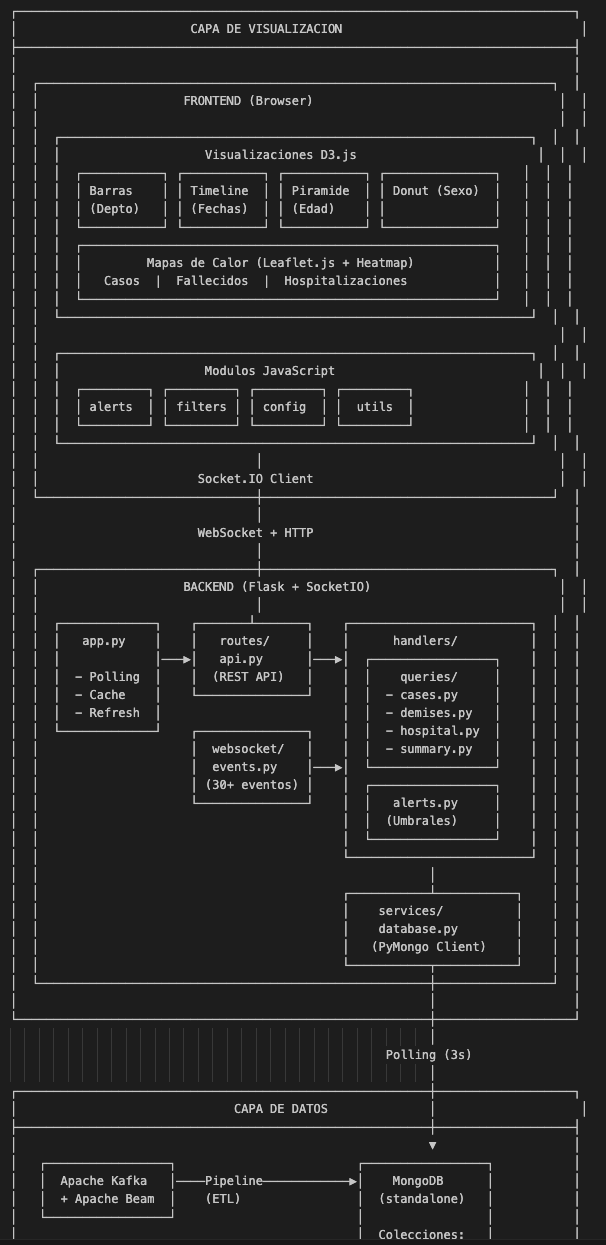
\includegraphics[width=0.95\textwidth]{images/dashboard-arquitectura.png}
\caption{Arquitectura del sistema de visualización en tiempo real}
\label{fig:dashboard-arquitectura}
\end{figure}

\subsubsection{Stack tecnológico del backend}

El servidor de visualización se implementa utilizando \textbf{Flask}, un microframework de Python que proporciona flexibilidad y simplicidad para construir aplicaciones web. La elección de Flask responde a su facilidad de integración con otras bibliotecas del ecosistema Python y su capacidad para manejar tanto endpoints REST como conexiones WebSocket.

Para la comunicación bidireccional en tiempo real se utiliza \textbf{Flask-SocketIO}, una extensión que implementa el protocolo WebSocket sobre Flask. Esta tecnología permite establecer conexiones persistentes entre el servidor y los clientes, habilitando la transmisión instantánea de actualizaciones cuando se detectan cambios en los datos.

La integración con \textbf{MongoDB} se realiza mediante \textbf{PyMongo}, el driver oficial de MongoDB para Python. El sistema aprovecha las capacidades de \textbf{Change Streams} de MongoDB para detectar modificaciones en las colecciones de datos en tiempo real, propagando automáticamente estos cambios a todos los clientes conectados.

\begin{lstlisting}[language=Python, caption={Configuración del servidor Flask con WebSocket}, label={lst:flask-config}]
from flask import Flask
from flask_socketio import SocketIO, emit
from pymongo import MongoClient

app = Flask(__name__)
socketio = SocketIO(app, cors_allowed_origins="*")

# Conexion a MongoDB
client = MongoClient(MONGO_URI)
db = client.covid_database

@socketio.on('connect')
def handle_connect():
    # Enviar datos iniciales al cliente
    emit('update_summary', get_summary_data())
    emit('update_department', get_cases_by_department())
\end{lstlisting}

\subsubsection{Stack tecnológico del frontend}

El frontend se desarrolla utilizando tecnologías web estándar optimizadas para la visualización de datos:

\begin{itemize}
    \item \textbf{D3.js (Data-Driven Documents)}: Biblioteca JavaScript para la manipulación de documentos basada en datos. Se utiliza para crear visualizaciones interactivas como gráficos de barras, líneas temporales y diagramas de distribución. D3.js proporciona control granular sobre cada elemento visual, permitiendo animaciones fluidas y transiciones durante las actualizaciones de datos.

    \item \textbf{Leaflet.js}: Biblioteca de código abierto para mapas interactivos. Se emplea para la representación de mapas de calor georreferenciados que muestran la distribución espacial de casos, fallecimientos y hospitalizaciones. La extensión \textbf{Leaflet.heat} permite generar visualizaciones de densidad sobre el mapa base.

    \item \textbf{Socket.IO Client}: Biblioteca JavaScript que implementa la comunicación WebSocket en el lado del cliente, permitiendo recibir actualizaciones en tiempo real desde el servidor sin necesidad de realizar polling.
\end{itemize}

\begin{lstlisting}[language=JavaScript, caption={Conexión WebSocket y manejo de eventos en el cliente}, label={lst:socketio-client}]
const socket = io();

socket.on('connect', () => {
    showConnectionStatus(true);
    socket.emit('get_alerts_config');
});

socket.on('update_department', (data) => {
    state.allDepartmentsData = data;
    renderDepartmentChart(data);
});

socket.on('filtered_age', (data) => {
    renderAgeChart(data);
});
\end{lstlisting}

\subsection{Diseño de dashboards}\label{diseuxf1o-de-dashboards}

El dashboard principal se organiza en secciones claramente diferenciadas que facilitan la comprensión del estado epidemiológico desde múltiples perspectivas. El diseño sigue principios de jerarquía visual, presentando primero los indicadores agregados más relevantes y posteriormente los análisis detallados.

\begin{figure}[H]
\centering
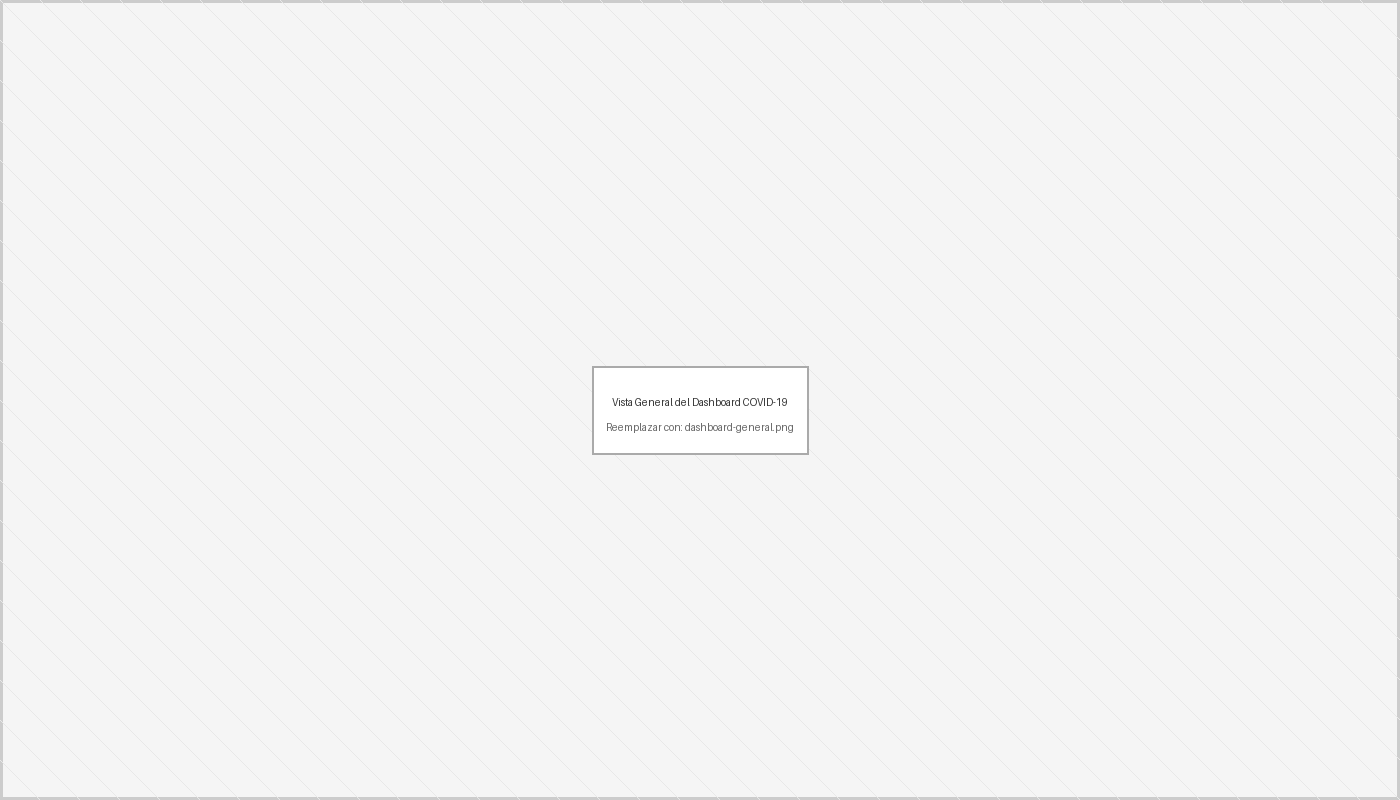
\includegraphics[width=0.98\textwidth]{images/dashboard-general.png}
\caption{Vista general del dashboard COVID-19 con indicadores en tiempo real}
\label{fig:dashboard-general}
\end{figure}

\subsubsection{Panel de indicadores clave (KPIs)}

En la parte superior del dashboard se presenta un panel con tarjetas de resumen que muestran los indicadores más relevantes:

\begin{itemize}
    \item \textbf{Total de Casos}: Número acumulado de casos registrados en el sistema.
    \item \textbf{Casos Positivos}: Total de casos confirmados con resultado positivo.
    \item \textbf{Hospitalizaciones}: Número de pacientes hospitalizados.
    \item \textbf{Fallecidos}: Total de decesos registrados.
    \item \textbf{Última Actualización}: Marca temporal de la última sincronización de datos.
\end{itemize}

Cada tarjeta incluye indicadores visuales que muestran la tendencia (incremento o decremento) respecto al período anterior, facilitando la interpretación rápida de la evolución de cada métrica.

\subsubsection{Panel de filtros interactivos}

El sistema implementa un panel lateral de filtros que permite segmentar los datos según diferentes criterios:

\begin{itemize}
    \item \textbf{Filtro por Sexo}: Permite visualizar datos segmentados por género (Masculino, Femenino, Todos).
    \item \textbf{Filtro por Departamento}: Lista desplegable con todos los departamentos del Perú, incluyendo contadores de casos por cada región.
    \item \textbf{Búsqueda de Departamento}: Campo de texto para filtrar rápidamente la lista de departamentos.
\end{itemize}

\begin{figure}[H]
\centering
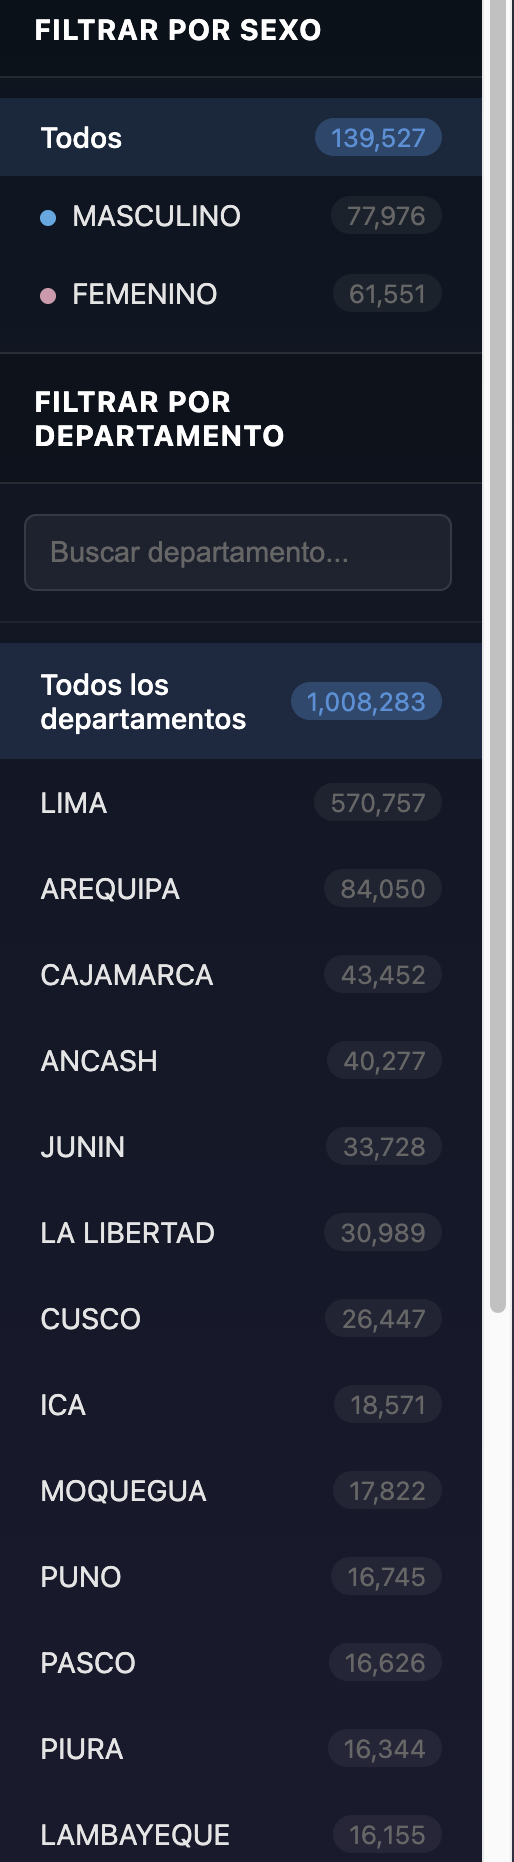
\includegraphics[width=0.3\textwidth]{images/filtros-laterales.png}
\caption{Panel de filtros interactivos para segmentación de datos}
\label{fig:filtros-laterales}
\end{figure}

La aplicación de filtros actualiza dinámicamente todas las visualizaciones del dashboard, solicitando datos filtrados al servidor mediante WebSocket y renderizando las nuevas gráficas sin necesidad de recargar la página.

\subsection{Reportes y visualizaciones implementadas}\label{reportes-visualizaciones}

El sistema implementa un conjunto completo de visualizaciones que cubren las principales dimensiones de análisis epidemiológico: distribución geográfica, temporal, demográfica y por severidad. Cada reporte se alimenta de consultas optimizadas a MongoDB utilizando el \emph{Aggregation Framework}, lo que permite procesar grandes volúmenes de datos de manera eficiente.

\subsubsection{Catálogo de reportes}

La Tabla \ref{tab:catalogo-reportes} presenta el catálogo completo de reportes implementados en el sistema, clasificados por categoría y tipo de visualización.

\begin{table}[H]
\centering
\small
\begin{tabular}{|l|l|l|l|}
\hline
\textbf{Reporte} & \textbf{Categoría} & \textbf{Visualización} & \textbf{Filtros} \\
\hline
Casos por Departamento & Casos & Barras horizontales & Sexo \\
Distribución por Sexo (Casos) & Casos & Donut & Departamento \\
Casos por Fecha & Casos & Línea temporal & Depto., Sexo \\
Casos por Grupo de Edad & Casos & Histograma & Departamento \\
Mapa de Calor Casos & Casos & Heatmap geográfico & Depto., Sexo \\
\hline
Fallecidos por Departamento & Fallecidos & Barras horizontales & Sexo \\
Distribución por Sexo (Fallecidos) & Fallecidos & Donut & Departamento \\
Fallecidos por Fecha & Fallecidos & Línea temporal & Depto., Sexo \\
Mapa de Calor Fallecidos & Fallecidos & Heatmap geográfico & Depto., Sexo \\
\hline
Mapa de Calor Hospitalizaciones & Hospitalizaciones & Heatmap geográfico & Depto., Sexo \\
\hline
\end{tabular}
\caption{Catálogo de reportes implementados en el sistema de visualización}
\label{tab:catalogo-reportes}
\end{table}

\subsubsection{Modelo de datos y colecciones}

Los reportes se alimentan de tres colecciones principales en MongoDB, cada una con un esquema específico adaptado al tipo de información epidemiológica:

\begin{itemize}
    \item \textbf{Colección \texttt{cases}}: Almacena los registros de pruebas diagnósticas de COVID-19. Campos principales: \texttt{departamento\_paciente}, \texttt{provincia\_paciente}, \texttt{distrito\_paciente}, \texttt{sexo}, \texttt{edad}, \texttt{fecha\_muestra}, \texttt{resultado}, \texttt{latitud}, \texttt{longitud}.

    \item \textbf{Colección \texttt{demises}}: Registra los fallecimientos confirmados por COVID-19. Campos principales: \texttt{departamento}, \texttt{provincia}, \texttt{distrito}, \texttt{sexo}, \texttt{edad}, \texttt{fecha\_fallecimiento}, \texttt{latitud}, \texttt{longitud}.

    \item \textbf{Colección \texttt{hospitalizations}}: Contiene información de pacientes hospitalizados. Campos principales: \texttt{dep\_domicilio}, \texttt{prov\_domicilio}, \texttt{dist\_domicilio}, \texttt{sexo}, \texttt{fecha\_ingreso\_hosp}, \texttt{latitud}, \texttt{longitud}.
\end{itemize}

\subsubsection{Casos por Departamento}

Este reporte presenta un gráfico de barras horizontales que muestra la distribución de casos confirmados por departamento. Los datos se ordenan de mayor a menor número de casos, facilitando la identificación rápida de las regiones más afectadas. El reporte muestra los 25 departamentos con mayor cantidad de casos.

\begin{figure}[H]
\centering
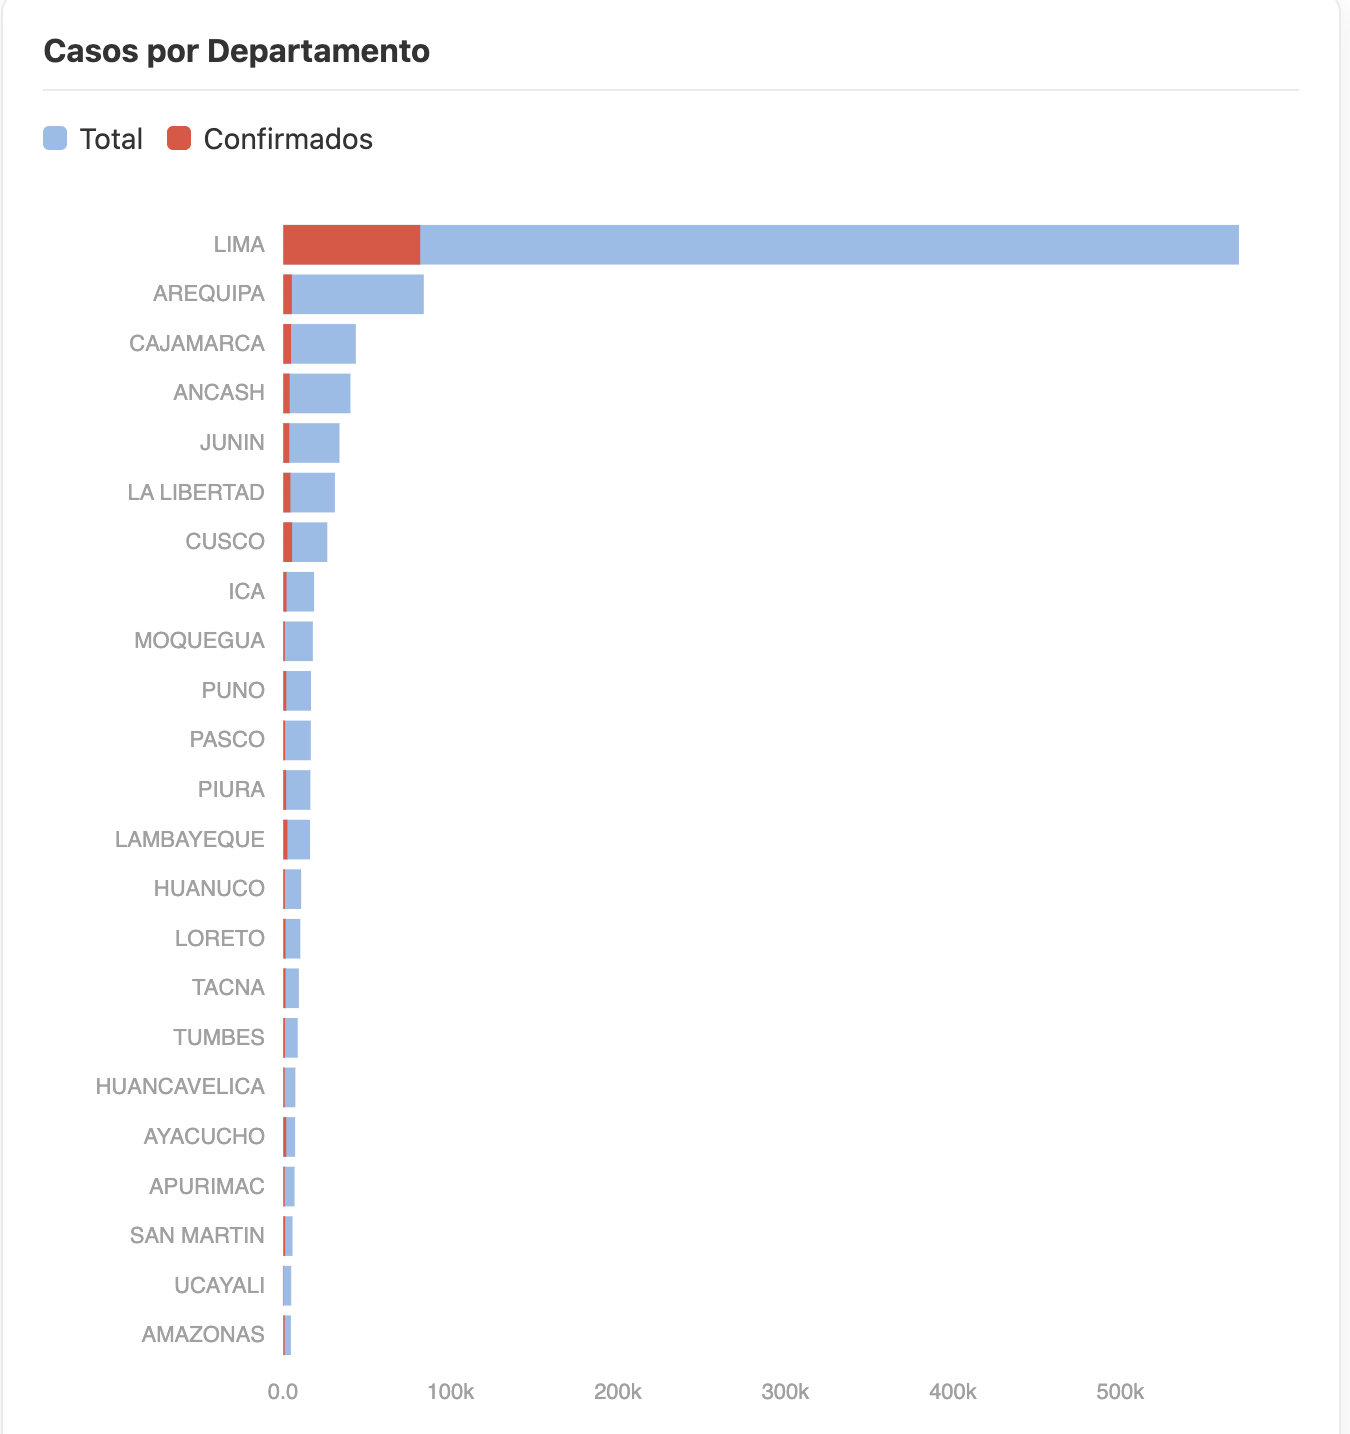
\includegraphics[width=0.7\textwidth]{images/casos-departamento.png}
\caption{Distribución de casos positivos por departamento}
\label{fig:casos-departamento}
\end{figure}

La consulta utiliza el \emph{Aggregation Framework} de MongoDB para agrupar, contar y ordenar los resultados:

\begin{lstlisting}[language=Python, caption={Consulta MongoDB para casos por departamento}, label={lst:cases-dept-query}]
def get_cases_by_department():
    pipeline = [
        {"$match": {"sexo": {"$nin": [None, "", "Sin especificar"]}}},
        {
            "$group": {
                "_id": "$departamento_paciente",
                "total": {"$sum": 1},
                "positivos": {
                    "$sum": {"$cond": [{"$eq": ["$resultado", "POSITIVO"]}, 1, 0]}
                }
            }
        },
        {"$sort": {"total": -1}},
        {"$limit": 25}
    ]

    results = []
    for r in db.cases.aggregate(pipeline):
        dept = r["_id"] or "Sin especificar"
        coords = DEPARTAMENTO_COORDS.get(dept.upper(), {"lat": None, "lon": None})
        results.append({
            "departamento": dept,
            "total": r["total"],
            "positivos": r["positivos"],
            "lat": coords["lat"],
            "lon": coords["lon"]
        })
    return results
\end{lstlisting}

La implementación del frontend utiliza D3.js para crear barras con transiciones animadas que reflejan los cambios en los datos:

\begin{lstlisting}[language=JavaScript, caption={Renderizado del gráfico de casos por departamento con D3.js}, label={lst:dept-chart}]
export function renderDepartmentChart(data) {
    const container = d3.select('#chart-department');
    container.selectAll('*').remove();

    const margin = { top: 20, right: 30, bottom: 40, left: 120 };
    const width = container.node().clientWidth - margin.left - margin.right;
    const height = Math.max(300, data.length * 25);

    const svg = container.append('svg')
        .attr('width', width + margin.left + margin.right)
        .attr('height', height + margin.top + margin.bottom)
        .append('g')
        .attr('transform', `translate(${margin.left},${margin.top})`);

    const x = d3.scaleLinear()
        .domain([0, d3.max(data, d => d.positivos)])
        .range([0, width]);

    const y = d3.scaleBand()
        .domain(data.map(d => d.departamento))
        .range([0, height])
        .padding(0.1);

    svg.selectAll('.bar')
        .data(data)
        .join('rect')
        .attr('class', 'bar')
        .attr('y', d => y(d.departamento))
        .attr('height', y.bandwidth())
        .attr('fill', COLORS.primary)
        .attr('x', 0)
        .attr('width', 0)
        .transition()
        .duration(750)
        .delay((d, i) => i * 30)
        .attr('width', d => x(d.positivos));
}
\end{lstlisting}

\subsubsection{Distribución por Sexo}

Se implementan dos gráficos de tipo \emph{donut} (anillo) que muestran la distribución porcentual de casos confirmados y fallecimientos según el sexo del paciente. Esta visualización permite identificar rápidamente disparidades de género en la afectación de la enfermedad.

\begin{figure}[H]
\centering
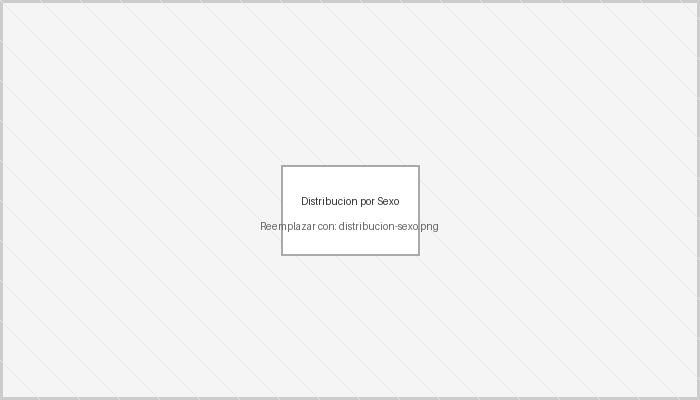
\includegraphics[width=0.6\textwidth]{images/distribucion-sexo.png}
\caption{Distribución de casos confirmados y fallecidos por sexo}
\label{fig:distribucion-sexo}
\end{figure}

La consulta para distribución por sexo filtra solo casos positivos y acepta filtrado por departamento:

\begin{lstlisting}[language=Python, caption={Consulta MongoDB para distribución por sexo}, label={lst:sex-query}]
def get_cases_by_sex(departamento: str = None):
    match_filter = {
        "sexo": {"$nin": [None, "", "Sin especificar"]},
        "resultado": "POSITIVO"
    }

    if departamento and departamento != "TODOS":
        match_filter["departamento_paciente"] = departamento

    pipeline = [
        {"$match": match_filter},
        {"$group": {"_id": "$sexo", "total": {"$sum": 1}}},
        {"$sort": {"total": -1}}
    ]
    return [{"sexo": r["_id"], "total": r["total"]}
            for r in db.cases.aggregate(pipeline)]
\end{lstlisting}

\subsubsection{Evolución Temporal de Casos}

El gráfico de línea temporal muestra la evolución de casos confirmados a lo largo del tiempo. Esta visualización resulta fundamental para identificar tendencias, picos epidémicos y el impacto de medidas de control. Los datos se limitan a los últimos 100 registros temporales para mantener la legibilidad.

\begin{figure}[H]
\centering
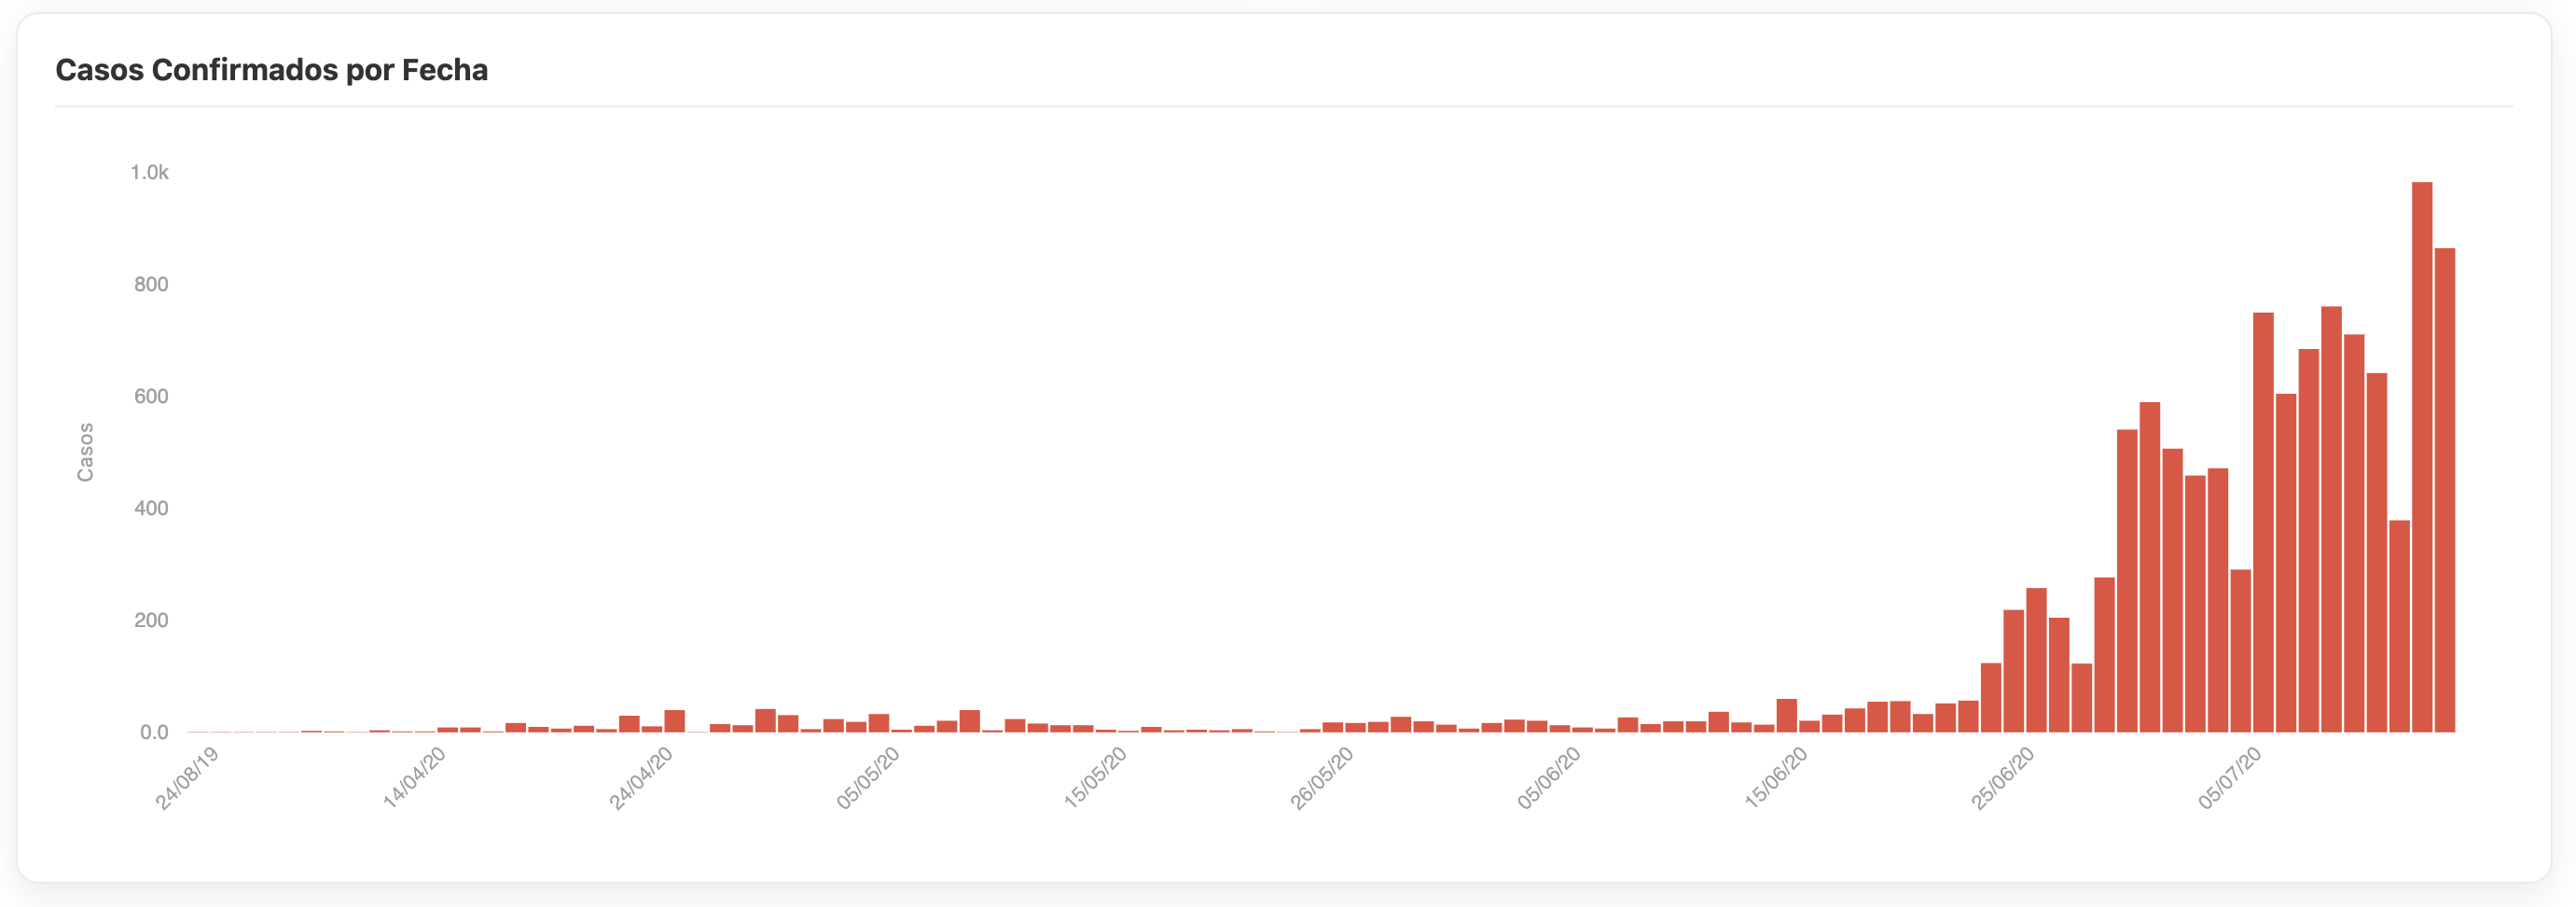
\includegraphics[width=0.85\textwidth]{images/casos-fecha.png}
\caption{Serie temporal de casos confirmados por fecha de muestra}
\label{fig:casos-fecha}
\end{figure}

\begin{lstlisting}[language=Python, caption={Consulta MongoDB para evolución temporal de casos}, label={lst:timeline-query}]
def get_cases_by_date(departamento: str = None, sexo: str = None):
    match_filter = {
        "sexo": {"$nin": [None, "", "Sin especificar"]},
        "resultado": "POSITIVO"
    }

    if departamento and departamento != "TODOS":
        match_filter["departamento_paciente"] = departamento

    if sexo and sexo != "TODOS":
        match_filter["sexo"] = sexo

    pipeline = [
        {"$match": match_filter},
        {"$group": {"_id": "$fecha_muestra", "total": {"$sum": 1}}},
        {"$sort": {"_id": 1}},
        {"$limit": 100}
    ]
    return [{"fecha": r["_id"], "total": r["total"], "positivos": r["total"]}
            for r in db.cases.aggregate(pipeline) if r["_id"]]
\end{lstlisting}

El gráfico incluye las siguientes funcionalidades interactivas implementadas con D3.js:
\begin{itemize}
    \item \textbf{Tooltip dinámico}: Al pasar el cursor sobre cada punto de la línea, se muestra un tooltip con la fecha exacta y el número de casos registrados.
    \item \textbf{Área sombreada}: Se renderiza un área con gradiente bajo la línea para mejorar la percepción visual de la magnitud y tendencia.
    \item \textbf{Ejes adaptativos}: El eje X formatea las fechas de manera inteligente según el rango temporal visualizado.
    \item \textbf{Transiciones animadas}: Los cambios en los datos se reflejan mediante transiciones suaves de 750ms.
\end{itemize}

\subsubsection{Casos por Grupo de Edad}

Este reporte presenta un histograma que agrupa los casos positivos por rangos etarios de 10 años (0-9, 10-19, 20-29, hasta 100+). La visualización permite identificar los grupos poblacionales más afectados por la enfermedad y analizar patrones demográficos.

\begin{figure}[H]
\centering
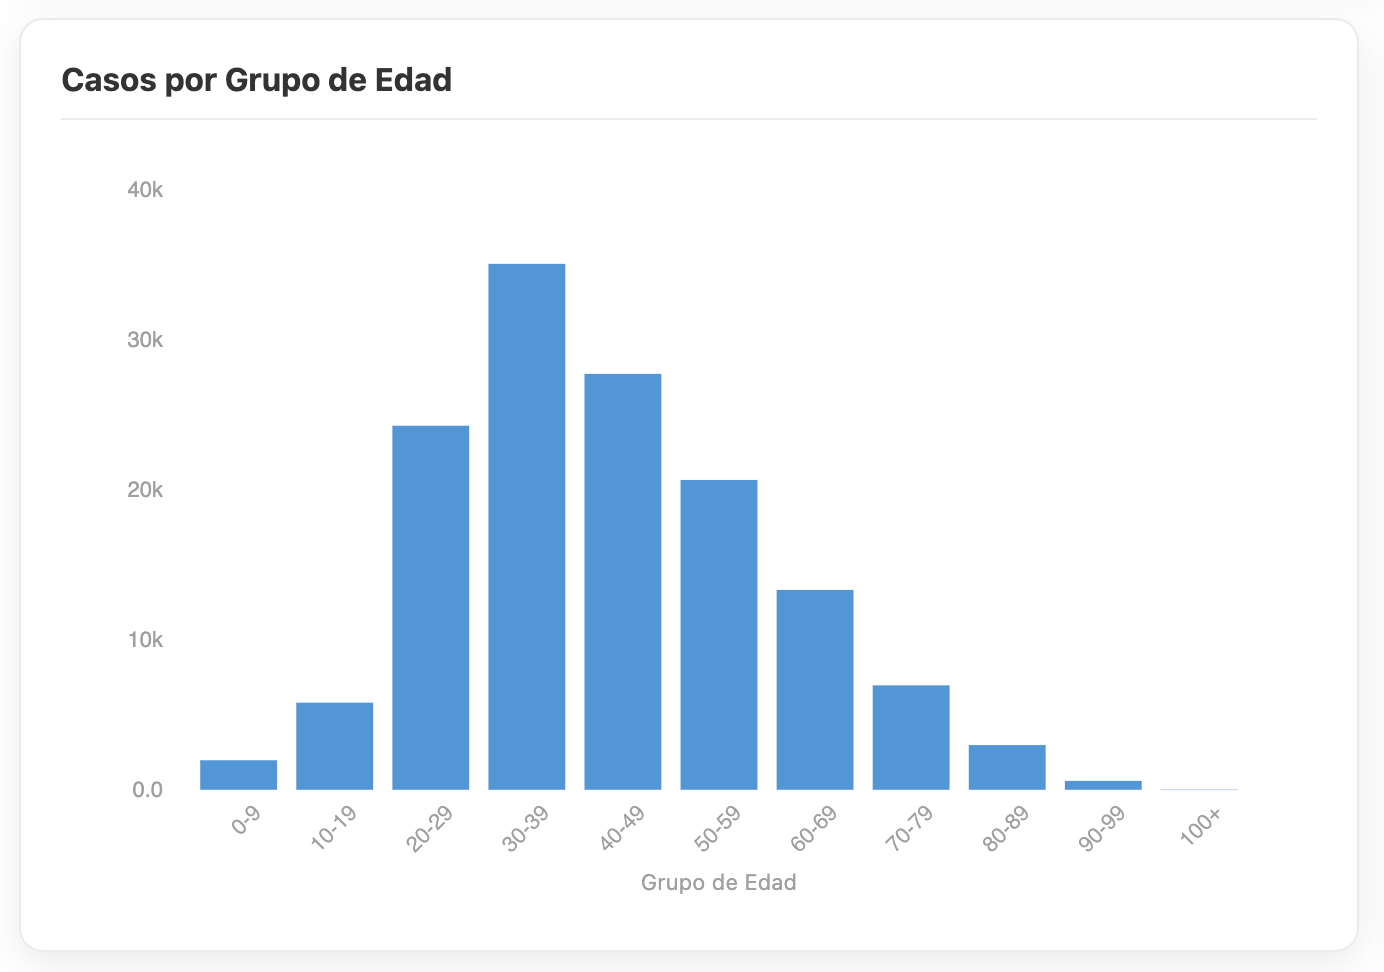
\includegraphics[width=0.7\textwidth]{images/casos-edad.png}
\caption{Distribución de casos positivos por grupo de edad}
\label{fig:casos-edad}
\end{figure}

Este gráfico se actualiza dinámicamente cuando se aplican filtros por departamento, mostrando únicamente los casos positivos de la región seleccionada. La consulta al backend utiliza el operador \texttt{\$bucket} del \emph{Aggregation Framework} para crear los rangos etarios:

\begin{lstlisting}[language=Python, caption={Consulta de casos por grupo de edad con operador \$bucket}, label={lst:age-query}]
def get_cases_by_age(departamento: str = None):
    match_filter = {
        "sexo": {"$nin": [None, "", "Sin especificar"]},
        "resultado": "POSITIVO"
    }

    if departamento and departamento != "TODOS":
        match_filter["departamento_paciente"] = departamento

    pipeline = [
        {"$match": match_filter},
        {
            "$bucket": {
                "groupBy": "$edad",
                "boundaries": [0, 10, 20, 30, 40, 50, 60, 70, 80, 90, 100],
                "default": "100+",
                "output": {"total": {"$sum": 1}}
            }
        }
    ]

    def label(r):
        return f"{r['_id']}-{r['_id']+9}" if isinstance(r["_id"], int) else r["_id"]

    return [{"grupo": label(r), "total": r["total"]}
            for r in db.cases.aggregate(pipeline)]
\end{lstlisting}

\subsubsection{Reportes de Fallecidos}

De manera análoga a los casos, se implementan visualizaciones específicas para el análisis de fallecimientos, utilizando la colección \texttt{demises}:

\paragraph{Fallecidos por Departamento}
Gráfico de barras horizontales con la distribución geográfica de decesos. Incluye coordenadas geográficas para integración con mapas.

\begin{lstlisting}[language=Python, caption={Consulta MongoDB para fallecidos por departamento}, label={lst:demises-dept}]
def get_demises_by_department():
    pipeline = [
        {"$match": {"sexo": {"$nin": [None, "", "Sin especificar"]}}},
        {
            "$group": {
                "_id": "$departamento",
                "total": {"$sum": 1},
                "lat": {"$max": "$latitud"},
                "lon": {"$max": "$longitud"}
            }
        },
        {"$sort": {"total": -1}},
        {"$limit": 25}
    ]
    # Enriquecimiento con coordenadas de respaldo
    for r in db.demises.aggregate(pipeline):
        if r.get("lat") is None:
            coords = DEPARTAMENTO_COORDS.get(r["_id"].upper())
            # Asignar coordenadas del diccionario de respaldo
\end{lstlisting}

\paragraph{Fallecidos por Fecha}
Serie temporal que muestra la evolución de la mortalidad diaria, permitiendo identificar picos de fallecimientos y correlacionarlos con olas epidémicas.

\paragraph{Fallecidos por Sexo}
Gráfico de anillo con la distribución por género, útil para análisis de mortalidad diferencial.

\begin{figure}[H]
\centering

\includegraphics[width=0.85\textwidth]{images/fallecidos-fecha.png}
\caption{Serie temporal de fallecidos por fecha de fallecimiento}
\label{fig:fallecidos-fecha}
\end{figure}

\subsubsection{Mapas de Calor Georreferenciados}

El sistema implementa tres mapas de calor interactivos que permiten visualizar la distribución espacial de los eventos epidemiológicos a nivel de distrito. Cada mapa utiliza un gradiente de colores que representa la intensidad: azul para baja concentración, pasando por verde y amarillo, hasta rojo para alta concentración.

\begin{enumerate}
    \item \textbf{Mapa de Calor de Casos}: Muestra la concentración geográfica de casos positivos, agregando datos a nivel de departamento, provincia y distrito.

    \item \textbf{Mapa de Calor de Fallecidos}: Visualiza la distribución espacial de decesos, permitiendo identificar zonas con mayor mortalidad.

    \item \textbf{Mapa de Calor de Hospitalizaciones}: Representa la ubicación de pacientes hospitalizados, útil para análisis de capacidad hospitalaria por región.
\end{enumerate}

\begin{figure}[H]
\centering
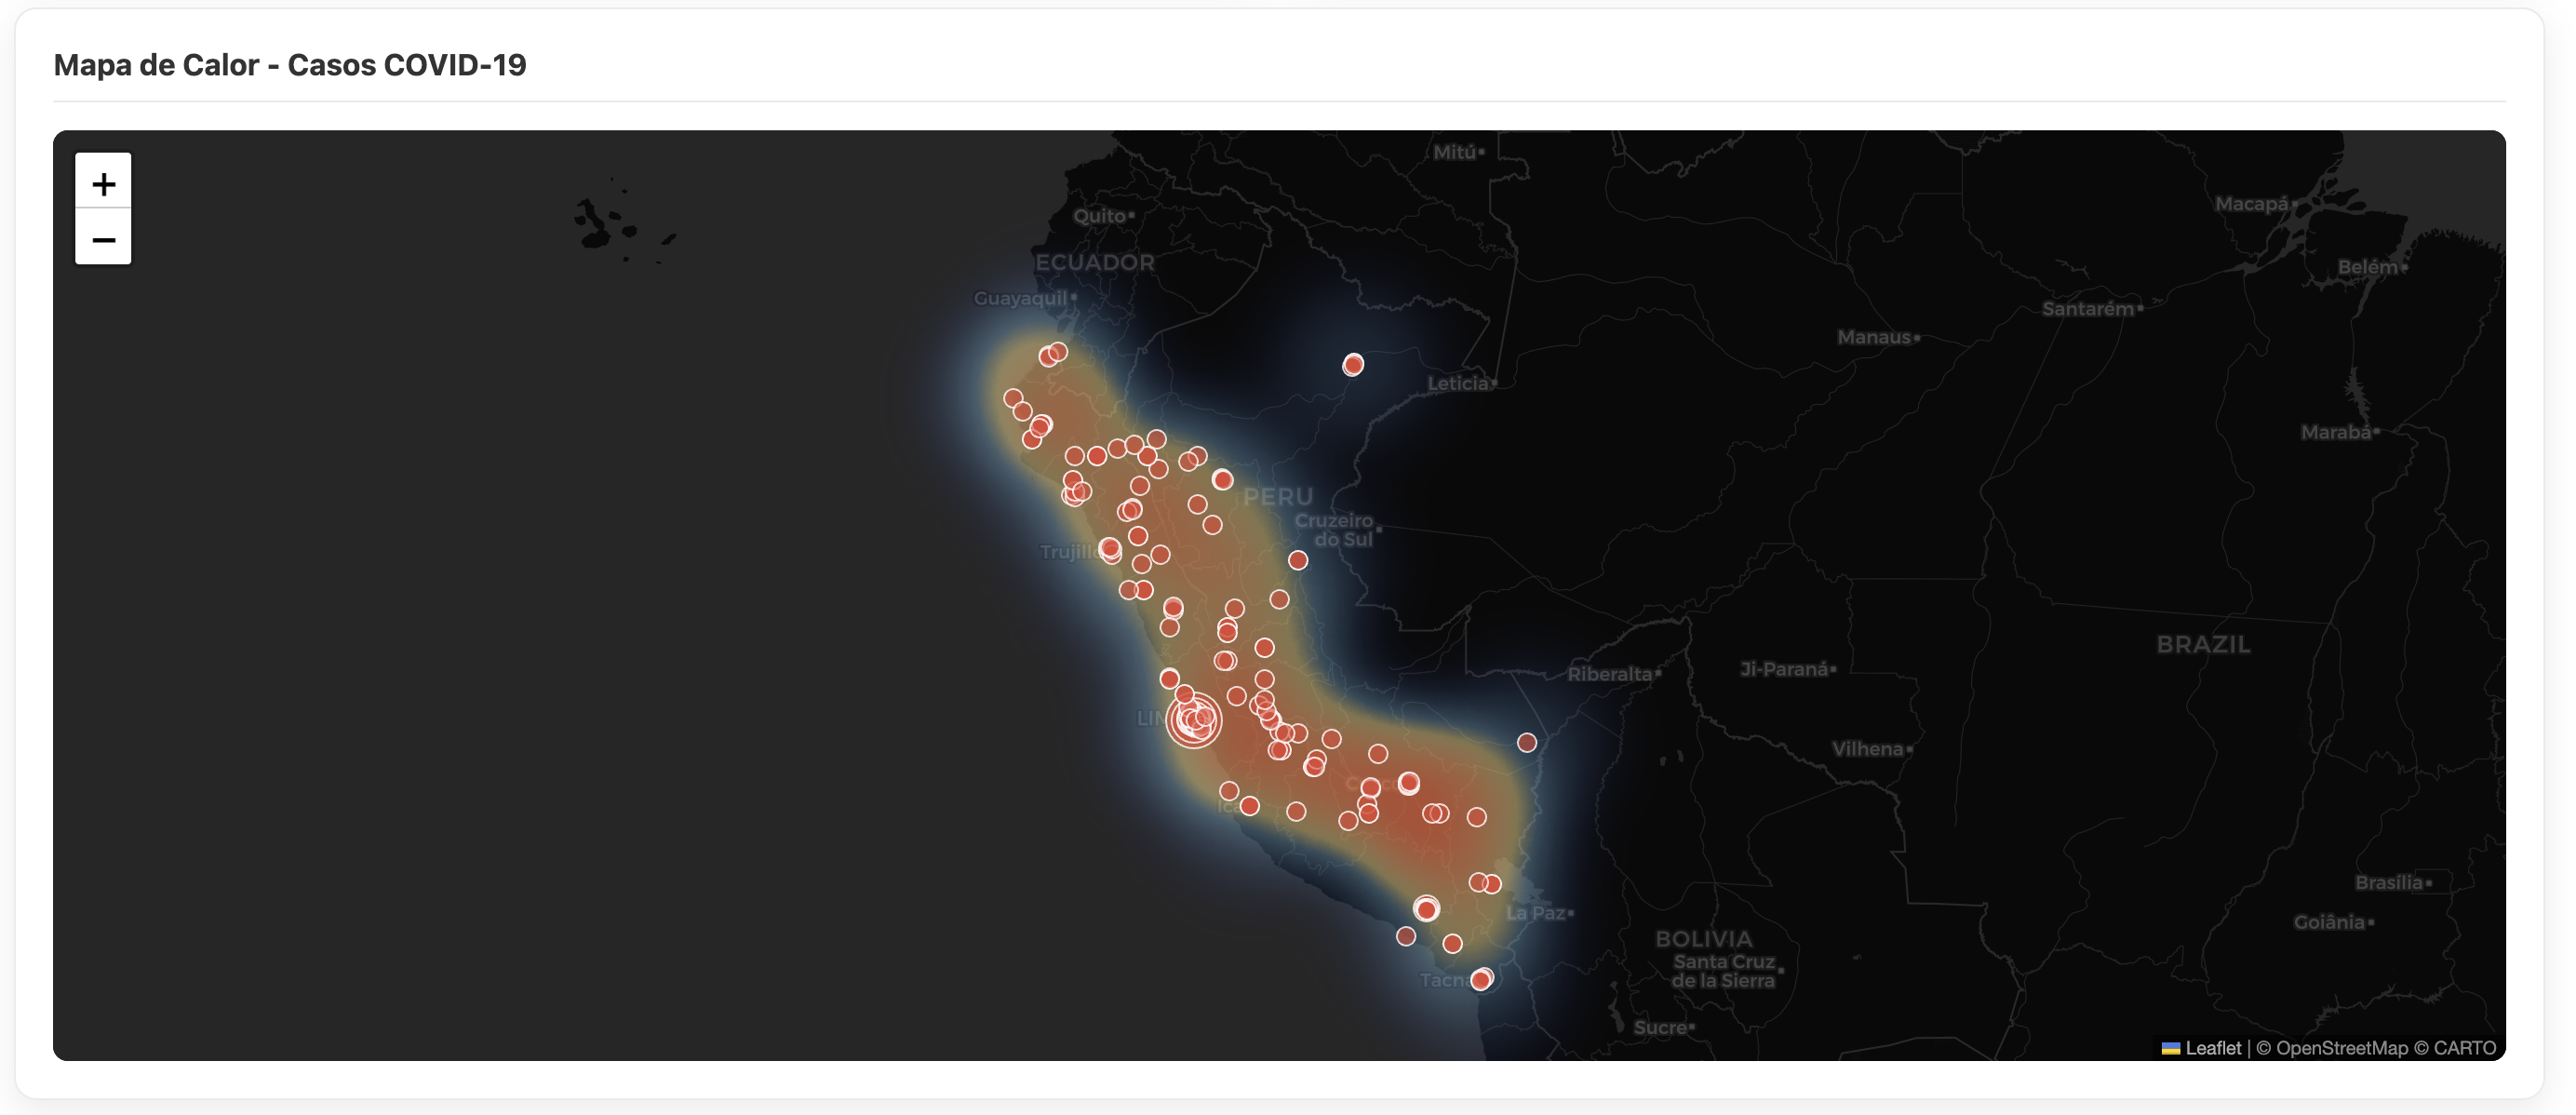
\includegraphics[width=0.85\textwidth]{images/mapa-calor-casos.png}
\caption{Mapa de calor de casos COVID-19 en Perú}
\label{fig:mapa-calor-casos}
\end{figure}

La consulta para el mapa de calor agrupa los datos a nivel de distrito y enriquece con coordenadas geográficas:

\begin{lstlisting}[language=Python, caption={Consulta MongoDB para datos del mapa de calor}, label={lst:heatmap-query}]
def get_heatmap_data():
    pipeline = [
        {"$match": {"sexo": {"$nin": [None, "", "Sin especificar"]}}},
        {
            "$group": {
                "_id": {
                    "departamento": "$departamento_muestra",
                    "provincia": "$provincia_muestra",
                    "distrito": "$distrito_muestra"
                },
                "total": {"$sum": 1},
                "positivos": {
                    "$sum": {"$cond": [{"$eq": ["$resultado", "POSITIVO"]}, 1, 0]}
                },
                "lat": {"$max": "$latitud"},
                "lon": {"$max": "$longitud"}
            }
        },
        {"$sort": {"total": -1}},
        {"$limit": 200}
    ]

    results = []
    for r in db.cases.aggregate(pipeline):
        lat, lon = r.get("lat"), r.get("lon")
        # Respaldo: obtener coordenadas del diccionario de ubigeos
        if lat is None or lon is None:
            coords = get_coords_from_ubigeo(
                r["_id"]["departamento"],
                r["_id"]["provincia"],
                r["_id"]["distrito"]
            )
            if coords:
                lat, lon = coords["lat"], coords["lon"]

        if lat and lon:
            results.append({...})
    return results
\end{lstlisting}

Los mapas se implementan utilizando \textbf{Leaflet.js} con la extensión \textbf{Leaflet.heat} para visualización de densidad:

\begin{lstlisting}[language=JavaScript, caption={Implementación del mapa de calor con Leaflet.js}, label={lst:heatmap-impl}]
export function renderHeatmap(data) {
    const container = document.getElementById('chart-heatmap');

    // Limpiar mapa existente si hay uno
    if (state.casesMap) {
        state.casesMap.remove();
    }

    // Crear nuevo mapa centrado en Peru
    state.casesMap = L.map('chart-heatmap').setView([-9.19, -75.0152], 5);

    // Capa base de OpenStreetMap
    L.tileLayer('https://{s}.tile.openstreetmap.org/{z}/{x}/{y}.png', {
        attribution: '&copy; OpenStreetMap contributors'
    }).addTo(state.casesMap);

    // Preparar datos para heatmap: [lat, lon, intensidad]
    const heatData = data
        .filter(d => d.lat && d.lon)
        .map(d => [d.lat, d.lon, d.positivos || d.total]);

    // Crear capa de calor con gradiente personalizado
    L.heatLayer(heatData, {
        radius: 25,
        blur: 15,
        maxZoom: 10,
        max: Math.max(...heatData.map(d => d[2])),
        gradient: {
            0.4: 'blue',
            0.6: 'lime',
            0.8: 'yellow',
            1.0: 'red'
        }
    }).addTo(state.casesMap);
}
\end{lstlisting}

\subsubsection{Sistema de coordenadas geográficas}

Las coordenadas geográficas se obtienen mediante un sistema de resolución en cascada:

\begin{enumerate}
    \item \textbf{Coordenadas del registro}: Si el documento original contiene campos \texttt{latitud} y \texttt{longitud}, se utilizan directamente.

    \item \textbf{Diccionario de ubigeos}: Se consulta un diccionario precomputado con las coordenadas del centroide de cada distrito del Perú, indexado por la combinación departamento-provincia-distrito.

    \item \textbf{Coordenadas de departamento}: Como último respaldo, se utilizan las coordenadas del centroide del departamento desde un diccionario de referencia.
\end{enumerate}

\begin{lstlisting}[language=Python, caption={Función de resolución de coordenadas por ubigeo}, label={lst:coords-resolution}]
def get_coords_from_ubigeo(departamento, provincia, distrito):
    """Obtiene coordenadas geograficas a partir del ubigeo."""
    key = f"{departamento}|{provincia}|{distrito}".upper()
    if key in UBIGEO_COORDS:
        return UBIGEO_COORDS[key]

    # Intentar con solo departamento y provincia
    key_prov = f"{departamento}|{provincia}|".upper()
    for k, v in UBIGEO_COORDS.items():
        if k.startswith(key_prov):
            return v

    # Respaldo: coordenadas del departamento
    return DEPARTAMENTO_COORDS.get(departamento.upper())
\end{lstlisting}

\subsection{Comunicación en tiempo real}\label{comunicacion-tiempo-real}

El sistema implementa un mecanismo de actualización en tiempo real basado en WebSockets y MongoDB Change Streams que permite reflejar instantáneamente cualquier cambio en los datos.

\subsubsection{Flujo de actualización de datos}

El flujo de actualización sigue los siguientes pasos:

\begin{enumerate}
    \item El pipeline de procesamiento Apache Beam inserta o actualiza documentos en MongoDB.
    \item MongoDB Change Streams detecta la modificación y notifica al servidor Flask.
    \item El servidor procesa el cambio y emite eventos WebSocket a todos los clientes conectados.
    \item Los clientes reciben los eventos y actualizan las visualizaciones correspondientes.
\end{enumerate}

\begin{figure}[H]
\centering
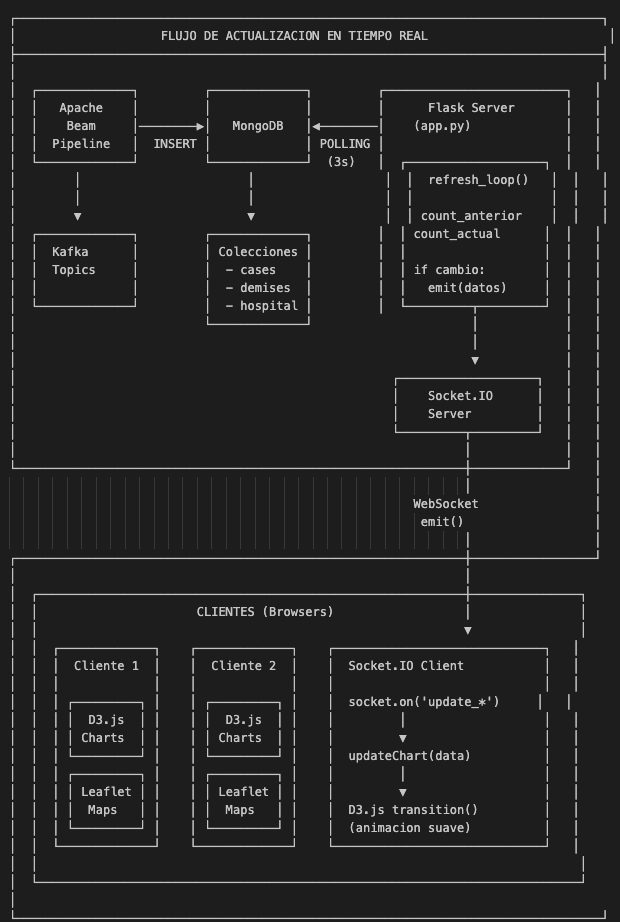
\includegraphics[width=0.9\textwidth]{images/flujo-realtime.png}
\caption{Flujo de actualización en tiempo real mediante WebSockets}
\label{fig:flujo-realtime}
\end{figure}

\subsubsection{Eventos WebSocket implementados}

El sistema define un conjunto de eventos para la comunicación bidireccional:

\begin{table}[H]
\centering
\begin{tabular}{|l|p{8cm}|}
\hline
\textbf{Evento} & \textbf{Descripción} \\
\hline
\texttt{update\_summary} & Actualiza las tarjetas de indicadores clave \\
\texttt{update\_department} & Actualiza el gráfico de casos por departamento \\
\texttt{update\_age} & Actualiza el histograma de grupos de edad \\
\texttt{update\_heatmap} & Actualiza el mapa de calor de casos \\
\texttt{filtered\_*} & Eventos para datos filtrados por departamento/sexo \\
\texttt{threshold\_alert} & Notifica una nueva alerta por umbral superado \\
\hline
\end{tabular}
\caption{Principales eventos WebSocket del sistema de visualización}
\label{tab:websocket-events}
\end{table}

\subsection{Sistema de alertas}\label{sistema-de-alertas}

El sistema de alertas constituye un componente proactivo que complementa la visualización pasiva de datos, permitiendo la detección automática de situaciones críticas que requieren atención inmediata.

\subsubsection{Arquitectura del sistema de alertas}

El sistema de alertas se integra directamente en el flujo de procesamiento de datos, evaluando cada actualización contra un conjunto de umbrales configurables. Cuando se detecta una condición de alerta, el sistema genera una notificación que se propaga instantáneamente a todos los clientes conectados.

\begin{figure}[H]
\centering
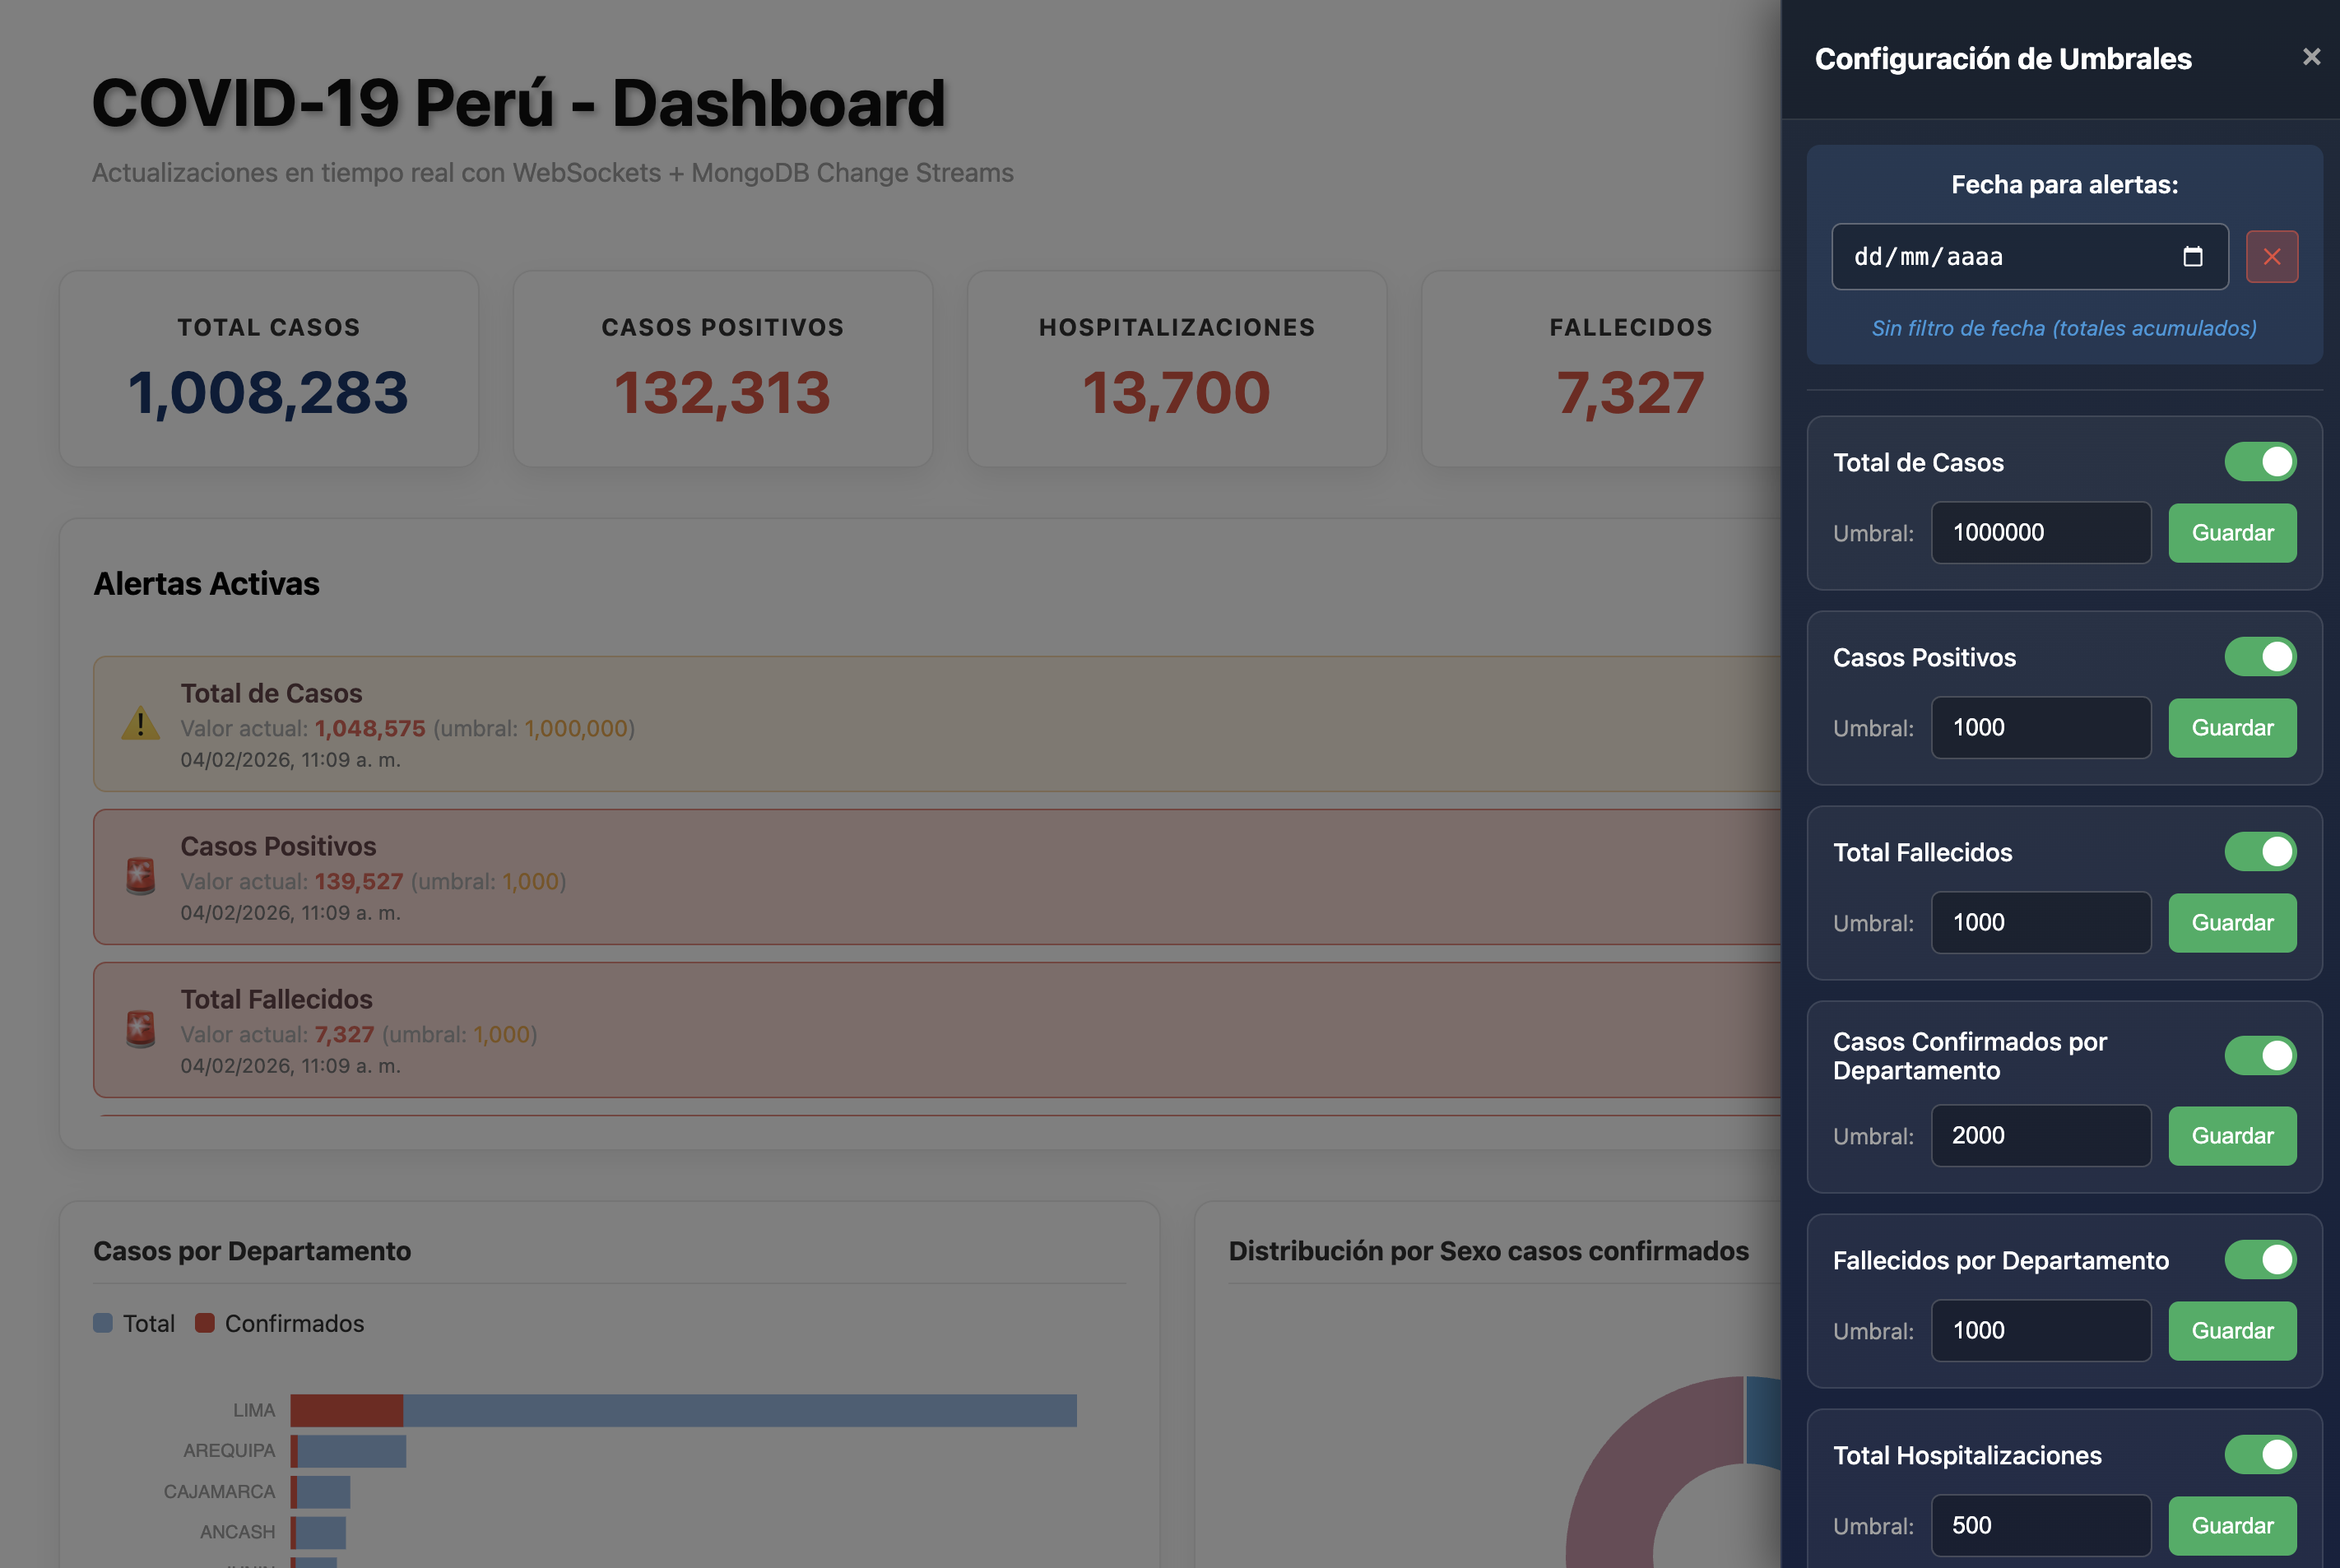
\includegraphics[width=0.85\textwidth]{images/sistema-alertas.png}
\caption{Panel de alertas activas y configuración de umbrales}
\label{fig:sistema-alertas}
\end{figure}

\subsubsection{Tipos de alertas implementadas}

El sistema implementa seis tipos de alertas configurables que cubren las principales métricas epidemiológicas. Cada tipo de alerta se define con un identificador único, un nombre descriptivo, un umbral por defecto y un estado de activación. La Tabla \ref{tab:tipos-alertas} presenta el detalle de cada tipo de alerta implementado.

\begin{table}[H]
\centering
\begin{tabular}{|l|l|r|p{5.5cm}|}
\hline
\textbf{Identificador} & \textbf{Nombre} & \textbf{Umbral} & \textbf{Descripción} \\
\hline
\texttt{cases\_total} & Total de Casos & 1,000,000 & Se activa cuando el número acumulado de casos registrados en el sistema supera el umbral definido. Permite monitorear el crecimiento general de la pandemia. \\
\hline
\texttt{cases\_positive} & Casos Positivos & 1,000 & Detecta incrementos significativos en el número de casos con resultado positivo confirmado por prueba de laboratorio. \\
\hline
\texttt{demises\_total} & Total Fallecidos & 1,000 & Alerta cuando el número acumulado de fallecimientos supera el umbral, indicando una situación de alta mortalidad. \\
\hline
\texttt{hospitalizations\_total} & Total Hospitalizaciones & 500 & Monitorea la capacidad hospitalaria alertando cuando el número de pacientes hospitalizados excede el límite configurado. \\
\hline
\texttt{cases\_by\_dept} & Casos por Departamento & 2,000 & Genera alertas específicas para cada departamento cuando los casos positivos en esa región superan el umbral. \\
\hline
\texttt{demises\_by\_dept} & Fallecidos por Departamento & 1,000 & Similar al anterior, pero enfocado en la mortalidad por región geográfica. \\
\hline
\end{tabular}
\caption{Tipos de alertas implementadas en el sistema de vigilancia epidemiológica}
\label{tab:tipos-alertas}
\end{table}

La configuración de alertas se almacena en una estructura de diccionario que permite su modificación en tiempo de ejecución:

\begin{lstlisting}[language=Python, caption={Configuración de tipos de alertas en el sistema}, label={lst:alerts-config}]
alerts_config = {
    "cases_total": {
        "enabled": True,
        "threshold": 1000000,
        "name": "Total de Casos"
    },
    "cases_positive": {
        "enabled": True,
        "threshold": 1000,
        "name": "Casos Positivos"
    },
    "demises_total": {
        "enabled": True,
        "threshold": 1000,
        "name": "Total Fallecidos"
    },
    "cases_by_dept": {
        "enabled": True,
        "threshold": 2000,
        "name": "Casos Confirmados por Departamento"
    },
    "demises_by_dept": {
        "enabled": True,
        "threshold": 1000,
        "name": "Fallecidos por Departamento"
    },
    "hospitalizations_total": {
        "enabled": True,
        "threshold": 500,
        "name": "Total Hospitalizaciones"
    }
}
\end{lstlisting}

\subsubsection{Niveles de severidad}

El sistema implementa un mecanismo de clasificación de alertas según su severidad, permitiendo priorizar la atención de situaciones más críticas. Se definen dos niveles:

\begin{itemize}
    \item \textbf{Nivel Warning (Advertencia)}: Se asigna cuando el valor actual supera el umbral pero se mantiene por debajo de 1.5 veces el umbral configurado. Indica una situación que requiere monitoreo pero no necesariamente acción inmediata.

    \item \textbf{Nivel Critical (Crítico)}: Se asigna cuando el valor actual supera 1.5 veces el umbral configurado. Indica una situación de emergencia que requiere atención inmediata.
\end{itemize}

El cálculo del nivel de severidad se realiza de forma automática en el momento de generación de la alerta:

\begin{lstlisting}[language=Python, caption={Cálculo del nivel de severidad de alertas}, label={lst:severity-calc}]
alert = {
    "id": f"{alert_key}_{int(datetime.now().timestamp())}",
    "metric": metric_key,
    "name": config.get("name", metric_key),
    "threshold": threshold,
    "current_value": current_value,
    "context": context,  # Departamento si aplica
    "date": date_display,
    "timestamp": datetime.now().isoformat(),
    "level": "warning" if current_value < threshold * 1.5 else "critical"
}
\end{lstlisting}

\subsubsection{Gestión thread-safe de alertas}

Dado que el sistema procesa múltiples eventos de forma concurrente a través de WebSockets, la gestión de alertas implementa mecanismos de sincronización mediante \texttt{threading.Lock} para garantizar la integridad de los datos en entornos multi-hilo:

\begin{lstlisting}[language=Python, caption={Implementación thread-safe del sistema de alertas}, label={lst:thread-safe}]
import threading

alerts_lock = threading.Lock()
active_alerts = []
alerts_history = []
MAX_ALERTS_HISTORY = 50

def check_threshold_alert(metric_key: str, current_value: int, context: str = None):
    with alerts_lock:
        config = alerts_config.get(metric_key)
        if not config or not config.get("enabled"):
            return None

        threshold = config.get("threshold", 0)
        if current_value >= threshold:
            # Verificar si ya existe una alerta activa para evitar duplicados
            existing = [a for a in active_alerts
                       if a["metric"] == metric_key and a.get("context") == context]
            if not existing:
                active_alerts.append(alert)
                alerts_history.insert(0, alert)
                if len(alerts_history) > MAX_ALERTS_HISTORY:
                    alerts_history.pop()
                return alert
\end{lstlisting}

\subsubsection{Filtrado temporal de alertas}

El sistema permite configurar una fecha global de referencia para el cálculo de alertas. Esta funcionalidad resulta especialmente útil para:

\begin{itemize}
    \item Analizar la situación epidemiológica en una fecha específica del pasado.
    \item Simular escenarios históricos y evaluar cómo habrían funcionado los umbrales.
    \item Comparar la evolución de métricas entre diferentes períodos.
\end{itemize}

Cuando se establece una fecha global, todas las consultas de verificación de umbrales filtran los datos por esa fecha específica:

\begin{lstlisting}[language=Python, caption={Verificación de alertas con filtrado temporal}, label={lst:alerts-date-filter}]
def check_all_thresholds(summary, dept_data=None, demises_dept=None, emit_callback=None):
    global_date = alerts_global_date

    # Total casos filtrado por fecha
    if global_date:
        count = get_count_by_date("cases", "fecha_muestra", global_date,
                                   {"sexo": {"$nin": [None, "", "Sin especificar"]}})
        alert = check_threshold_alert("cases_total", count)
    else:
        alert = check_threshold_alert("cases_total", summary.get("cases_total", 0))

    # Casos por departamento filtrado por fecha
    if global_date:
        filtered_dept = get_dept_count_by_date("cases", "departamento_paciente",
                                                "fecha_muestra", global_date,
                                                count_field="positivos")
        for dept in filtered_dept[:5]:
            alert = check_threshold_alert("cases_by_dept", dept.get("positivos", 0),
                                          context=dept.get("departamento"))
\end{lstlisting}

\subsubsection{Configuración dinámica de umbrales}

El dashboard incluye un panel de configuración accesible mediante el botón de engranaje en la sección de alertas. Este panel permite ajustar los umbrales de cada alerta en tiempo real sin necesidad de reiniciar el servidor. Las modificaciones se propagan instantáneamente a todos los clientes conectados mediante WebSocket.

Los usuarios pueden realizar las siguientes acciones de configuración:

\begin{itemize}
    \item \textbf{Activar/Desactivar alertas}: Cada tipo de alerta puede habilitarse o deshabilitarse individualmente mediante un interruptor (\emph{toggle}).

    \item \textbf{Modificar umbrales}: El valor numérico del umbral puede ajustarse mediante un campo de entrada. Los cambios se guardan automáticamente.

    \item \textbf{Establecer fecha de referencia}: Un selector de fecha permite configurar la fecha global para el cálculo de todas las alertas.

    \item \textbf{Limpiar fecha}: Botón para eliminar el filtro temporal y volver al modo de alertas acumuladas.
\end{itemize}

La actualización de configuración se realiza mediante eventos WebSocket bidireccionales:

\begin{lstlisting}[language=Python, caption={Manejador WebSocket para actualización de umbrales}, label={lst:update-threshold}]
@socketio.on('update_alert_threshold')
def handle_update_alert_threshold(data):
    metric = data.get("metric")
    if metric not in alerts_config:
        emit('error', {'message': f'Metrica desconocida: {metric}'})
        return

    update_alert_config(
        metric,
        threshold=int(data["threshold"]) if "threshold" in data else None,
        enabled=bool(data["enabled"]) if "enabled" in data else None
    )

    config_data = {
        "config": get_alerts_config(),
        "global_date": get_alerts_global_date()
    }
    emit('alerts_config', config_data)
    socketio.emit('alerts_config_updated', config_data)
\end{lstlisting}

\subsubsection{Historial de alertas}

El sistema mantiene un historial de las últimas 50 alertas generadas, permitiendo revisar eventos pasados incluso después de que hayan sido descartados de la lista de alertas activas. Este historial incluye:

\begin{itemize}
    \item Marca temporal de generación de la alerta.
    \item Métrica y contexto (departamento) asociado.
    \item Valor que disparó la alerta y umbral configurado en ese momento.
    \item Nivel de severidad asignado.
\end{itemize}

\subsubsection{Visualización de alertas}

Las alertas activas se muestran en un panel dedicado en la parte superior del dashboard, con indicadores visuales que destacan su severidad. El panel de alertas incluye:

\begin{itemize}
    \item \textbf{Indicador de color}: Las alertas de nivel \texttt{critical} se muestran con borde rojo y fondo rosado. Las alertas de nivel \texttt{warning} utilizan borde amarillo y fondo amarillo claro.

    \item \textbf{Información contextual}: Cada alerta muestra el nombre de la métrica, el valor actual, el umbral superado y, en caso de alertas por departamento, el nombre de la región afectada.

    \item \textbf{Marca temporal}: Se muestra la hora exacta en que se generó la alerta, facilitando el seguimiento cronológico de eventos.

    \item \textbf{Fecha de referencia}: Si se configuró una fecha global, se muestra junto a la alerta para contextualizar el período analizado.

    \item \textbf{Botón de descarte}: Permite al usuario marcar la alerta como revisada y eliminarla de la lista de alertas activas.
\end{itemize}

\begin{figure}[H]
\centering

\includegraphics[width=0.9\textwidth]{images/alertas-panel-detalle.png}
\caption{Panel de alertas activas mostrando diferentes niveles de severidad}
\label{fig:alertas-panel-detalle}
\end{figure}

\subsubsection{Notificaciones en tiempo real}

Cuando se genera una nueva alerta, el sistema implementa múltiples mecanismos de notificación para asegurar que las situaciones críticas no pasen desapercibidas:

\begin{enumerate}
    \item \textbf{Notificación emergente (Toast)}: Se muestra una notificación en la esquina superior derecha de la pantalla durante 5 segundos, con el resumen de la alerta generada.

    \item \textbf{Actualización del panel de alertas}: La nueva alerta se añade automáticamente al panel de alertas activas con una animación de entrada.

    \item \textbf{Indicador visual en el header}: El contador de alertas activas se actualiza y muestra un badge con el número de alertas pendientes de revisión.

    \item \textbf{Emisión broadcast}: La alerta se propaga a todos los clientes conectados simultáneamente mediante el evento \texttt{threshold\_alert}.
\end{enumerate}

\begin{lstlisting}[language=JavaScript, caption={Manejo de notificaciones de alerta en el cliente}, label={lst:alert-notification}]
socket.on('threshold_alert', (alert) => {
    console.log('[WebSocket] Nueva alerta:', alert);
    state.activeAlerts.push(alert);
    renderActiveAlerts();
    showAlertNotification(alert);
});

function showAlertNotification(alert) {
    const levelClass = alert.level === 'critical' ? 'toast-critical' : 'toast-warning';
    const toast = document.createElement('div');
    toast.className = `toast ${levelClass}`;
    toast.innerHTML = `
        <strong>${alert.name}</strong>
        <p>Valor: ${alert.current_value} (Umbral: ${alert.threshold})</p>
        ${alert.context ? `<p>Departamento: ${alert.context}</p>` : ''}
    `;
    document.getElementById('notifications').appendChild(toast);
    setTimeout(() => toast.remove(), 5000);
}
\end{lstlisting}

\subsubsection{Gestión de alertas activas}

El sistema proporciona funcionalidades para la gestión del ciclo de vida de las alertas:

\begin{itemize}
    \item \textbf{Descarte individual}: Cada alerta puede descartarse individualmente mediante el botón de cierre, indicando que ha sido revisada por el usuario.

    \item \textbf{Limpieza masiva}: El botón ``Limpiar todo'' permite eliminar todas las alertas activas de una vez.

    \item \textbf{Actualización automática}: Cuando una métrica que previamente superaba el umbral vuelve a valores normales, la alerta correspondiente puede actualizarse o eliminarse automáticamente.

    \item \textbf{Prevención de duplicados}: El sistema verifica la existencia de alertas activas para la misma métrica y contexto antes de crear una nueva, actualizando el valor en lugar de generar duplicados.
\end{itemize}

En conjunto, el sistema de alertas refuerza el carácter proactivo de la plataforma de visualización, transformándola de una herramienta de consulta pasiva a un sistema de vigilancia activa que apoya la detección temprana de situaciones críticas. La combinación de umbrales configurables, niveles de severidad, filtrado temporal y notificaciones en tiempo real proporciona una solución completa para el monitoreo epidemiológico.

\subsection{Stack tecnológico del sistema de visualización}\label{stack-tecnologico-completo}

El sistema de visualización se construye sobre un conjunto de tecnologías modernas seleccionadas por su capacidad de integración, rendimiento y soporte para comunicación en tiempo real. La Tabla \ref{tab:stack-tecnologico} presenta el inventario completo de tecnologías utilizadas, clasificadas por capa arquitectónica.

\begin{table}[H]
\centering
\small
\begin{tabular}{|l|l|l|p{5cm}|}
\hline
\textbf{Capa} & \textbf{Tecnología} & \textbf{Versión} & \textbf{Propósito} \\
\hline
\multirow{4}{*}{Backend} & Python & 3.11+ & Lenguaje de programación principal \\
& Flask & 2.3+ & Framework web para API REST \\
& Flask-SocketIO & 5.3+ & Extensión para WebSockets \\
& PyMongo & 4.5+ & Driver de MongoDB para Python \\
\hline
\multirow{4}{*}{Frontend} & HTML5/CSS3 & - & Estructura y estilos \\
& JavaScript ES6+ & - & Lógica de cliente \\
& D3.js & 7.x & Visualización de datos \\
& Leaflet.js & 1.9+ & Mapas interactivos \\
& Socket.IO Client & 4.7+ & Cliente WebSocket \\
\hline
\multirow{2}{*}{Base de Datos} & MongoDB & 6.0+ & Almacenamiento NoSQL \\
& Change Streams & - & Detección de cambios en tiempo real \\
\hline
\multirow{2}{*}{Comunicación} & WebSocket & RFC 6455 & Protocolo bidireccional \\
& REST API & HTTP/1.1 & Endpoints de consulta \\
\hline
\end{tabular}
\caption{Stack tecnológico completo del sistema de visualización}
\label{tab:stack-tecnologico}
\end{table}

\subsubsection{Justificación de las tecnologías seleccionadas}

\paragraph{Flask como framework web}
Se selecciona Flask por su naturaleza minimalista y su filosofía de microframework, lo que permite integrar únicamente los componentes necesarios sin la sobrecarga de frameworks más completos. Flask proporciona:
\begin{itemize}
    \item Routing flexible para definir endpoints REST.
    \item Sistema de plantillas Jinja2 para renderizado de HTML.
    \item Extensibilidad mediante blueprints para organización modular.
    \item Compatibilidad nativa con WSGI para despliegue en producción.
\end{itemize}

\paragraph{WebSockets para comunicación en tiempo real}
La elección de WebSockets sobre alternativas como Server-Sent Events (SSE) o Long Polling responde a la necesidad de comunicación bidireccional. WebSocket permite:
\begin{itemize}
    \item Conexión persistente con menor overhead que HTTP.
    \item Comunicación bidireccional (servidor $\leftrightarrow$ cliente).
    \item Latencia reducida para actualizaciones en tiempo real.
    \item Soporte para múltiples canales de eventos.
\end{itemize}

\paragraph{D3.js para visualización}
D3.js se selecciona por su control granular sobre los elementos SVG, permitiendo crear visualizaciones personalizadas que no serían posibles con bibliotecas de alto nivel. Sus ventajas incluyen:
\begin{itemize}
    \item Bindeo de datos a elementos del DOM (\emph{data binding}).
    \item Sistema de transiciones para animaciones fluidas.
    \item Escalas y ejes configurables para cualquier tipo de dato.
    \item Soporte para múltiples tipos de gráficos (barras, líneas, áreas, donut).
\end{itemize}

\paragraph{MongoDB como base de datos}
MongoDB se integra naturalmente con el pipeline de procesamiento Apache Beam y ofrece:
\begin{itemize}
    \item Esquema flexible para datos epidemiológicos heterogéneos.
    \item Aggregation Framework para consultas analíticas complejas.
    \item Change Streams para detección de cambios en tiempo real.
    \item Escalabilidad horizontal mediante sharding.
\end{itemize}

\subsection{Arquitectura de módulos del sistema}\label{arquitectura-modulos}

El sistema de visualización se organiza en una arquitectura modular que separa responsabilidades y facilita el mantenimiento. La Figura \ref{fig:arquitectura-modulos} ilustra la organización de los principales módulos.

\begin{figure}[H]
\centering
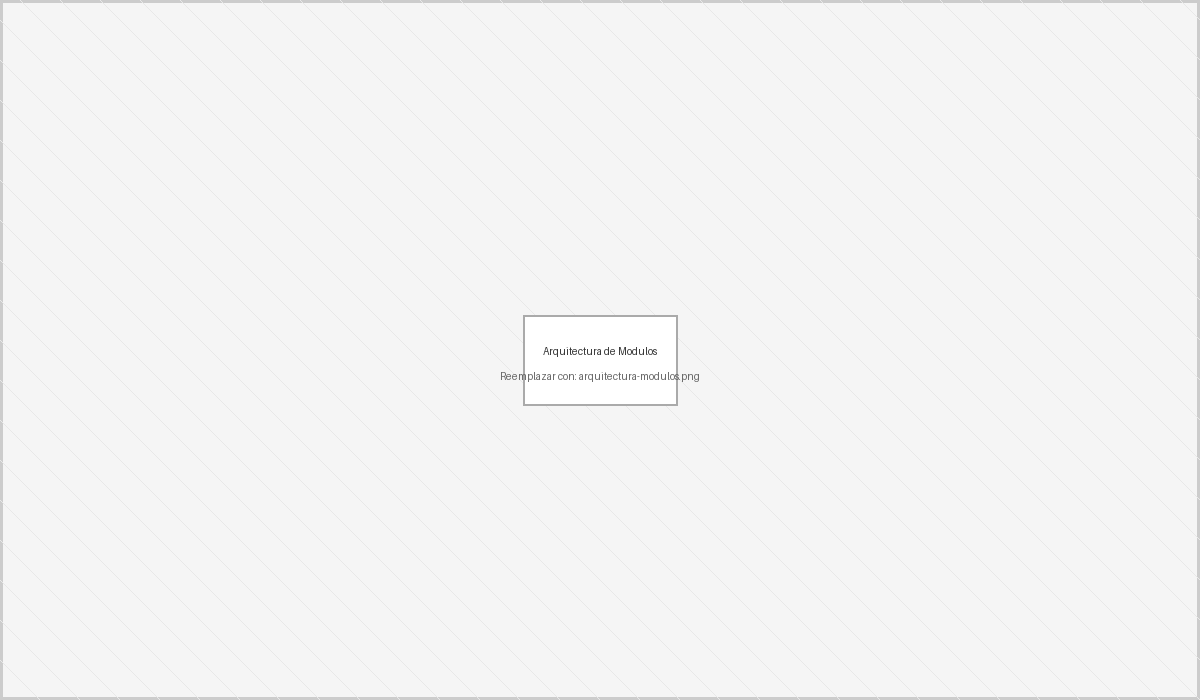
\includegraphics[width=0.95\textwidth]{images/arquitectura-modulos.png}
\caption{Arquitectura de módulos del sistema de visualización}
\label{fig:arquitectura-modulos}
\end{figure}

\subsubsection{Módulos del backend}

El backend se estructura en los siguientes módulos principales:

\paragraph{Módulo de Servicios (\texttt{services/})}
Contiene la lógica de conexión y configuración de servicios externos:
\begin{itemize}
    \item \texttt{database.py}: Gestiona la conexión a MongoDB mediante PyMongo, implementando el patrón Singleton para reutilizar la conexión.
\end{itemize}

\begin{lstlisting}[language=Python, caption={Módulo de conexión a base de datos}, label={lst:db-service}]
# services/database.py
from pymongo import MongoClient
from config import MONGO_URI, DATABASE

mongo_client = None
db = None

try:
    mongo_client = MongoClient(MONGO_URI, serverSelectionTimeoutMS=1000)
    mongo_client.admin.command("ping")
    db = mongo_client[DATABASE]
    print(f"[Mongo] Conectado a {MONGO_URI}")
except Exception as e:
    print(f"[Mongo] No se pudo conectar: {e}")
\end{lstlisting}

\paragraph{Módulo de Consultas (\texttt{handlers/queries/})}
Implementa las funciones de acceso a datos organizadas por dominio:
\begin{itemize}
    \item \texttt{summary.py}: Consultas de indicadores agregados (KPIs).
    \item \texttt{cases.py}: Consultas relacionadas con casos COVID-19.
    \item \texttt{demises.py}: Consultas de datos de fallecimientos.
    \item \texttt{hospitalizations.py}: Consultas de hospitalizaciones.
\end{itemize}

\paragraph{Módulo de Alertas (\texttt{handlers/alerts.py})}
Centraliza toda la lógica del sistema de alertas:
\begin{itemize}
    \item Configuración y gestión de umbrales.
    \item Verificación de condiciones de alerta.
    \item Gestión del ciclo de vida de alertas activas.
    \item Historial de alertas generadas.
\end{itemize}

\paragraph{Módulo de WebSocket (\texttt{handlers/websocket/})}
Gestiona los eventos de comunicación en tiempo real:
\begin{itemize}
    \item \texttt{events.py}: Registra los manejadores de eventos WebSocket.
    \item Maneja conexiones, desconexiones y solicitudes de datos.
    \item Emite actualizaciones a clientes conectados.
\end{itemize}

\paragraph{Módulo de Rutas (\texttt{routes/})}
Define los endpoints REST de la API:
\begin{itemize}
    \item \texttt{api.py}: Blueprint con rutas para consultas HTTP.
    \item Endpoints para datos iniciales y configuración.
\end{itemize}

\subsubsection{Módulos del frontend}

El frontend se organiza en módulos ES6 que facilitan la separación de responsabilidades:

\paragraph{Módulo de Configuración (\texttt{modules/config.js})}
Define constantes globales, paleta de colores y estado de la aplicación:

\begin{lstlisting}[language=JavaScript, caption={Módulo de configuración del frontend}, label={lst:config-module}]
// modules/config.js
export const COLORS = {
    primary: '#3498db',
    secondary: '#2ecc71',
    danger: '#e74c3c',
    warning: '#f39c12',
    info: '#9b59b6'
};

export const state = {
    isConnected: false,
    selectedDepartment: 'TODOS',
    selectedSex: 'TODOS',
    allDepartmentsData: [],
    allSexData: [],
    allAgeData: [],
    allTimelineData: [],
    allHeatmapData: [],
    activeAlerts: [],
    alertsConfig: {}
};
\end{lstlisting}

\paragraph{Módulo de Utilidades (\texttt{modules/utils.js})}
Funciones auxiliares reutilizables:
\begin{itemize}
    \item \texttt{formatNumber()}: Formato de números con separadores de miles.
    \item \texttt{showConnectionStatus()}: Actualiza indicador de conexión.
    \item \texttt{showNotification()}: Muestra notificaciones toast.
    \item \texttt{filterValidDepts()}: Filtra departamentos válidos.
\end{itemize}

\paragraph{Módulo de Filtros (\texttt{modules/filters.js})}
Gestiona la lógica de filtrado interactivo:
\begin{itemize}
    \item Renderizado de listas de filtros.
    \item Aplicación de filtros a visualizaciones.
    \item Actualización de indicadores de filtro activo.
    \item Comunicación con servidor para datos filtrados.
\end{itemize}

\paragraph{Módulo de Alertas (\texttt{modules/alerts.js})}
Implementa la interfaz de usuario del sistema de alertas:
\begin{itemize}
    \item Renderizado del panel de alertas activas.
    \item Configuración de umbrales mediante formularios.
    \item Notificaciones visuales de nuevas alertas.
    \item Gestión de descarte y limpieza de alertas.
\end{itemize}

\paragraph{Módulos de Gráficos (\texttt{charts/})}
Cada tipo de visualización se implementa en un módulo independiente:
\begin{itemize}
    \item \texttt{department.js}: Gráficos de barras por departamento.
    \item \texttt{sex.js}: Gráficos donut de distribución por sexo.
    \item \texttt{timeline.js}: Series temporales de evolución.
    \item \texttt{age.js}: Histogramas de grupos de edad.
    \item \texttt{heatmaps.js}: Mapas de calor georreferenciados.
\end{itemize}

\subsection{Flujo de datos end-to-end}\label{flujo-datos-end-to-end}

El flujo de datos del sistema de visualización se integra con el pipeline de procesamiento de datos, formando un ciclo completo desde la ingesta de datos brutos hasta su presentación visual al usuario final.

\subsubsection{Diagrama de flujo completo}

\begin{figure}[H]
\centering

\includegraphics[width=0.98\textwidth]{images/flujo-datos-completo.png}
\caption{Flujo de datos end-to-end del sistema de vigilancia epidemiológica}
\label{fig:flujo-datos-completo}
\end{figure}

\subsubsection{Etapas del flujo de datos}

\paragraph{1. Ingesta de datos}
Los datos epidemiológicos se obtienen de fuentes oficiales (Ministerio de Salud del Perú) en formato CSV. El sistema de ingesta:
\begin{itemize}
    \item Lee archivos de casos, fallecimientos y hospitalizaciones.
    \item Valida la estructura y calidad de los datos.
    \item Publica los registros en topics de Apache Kafka.
\end{itemize}

\paragraph{2. Procesamiento con Apache Beam}
El pipeline de procesamiento implementa transformaciones sobre los datos:
\begin{itemize}
    \item Limpieza y normalización de campos.
    \item Enriquecimiento con coordenadas geográficas.
    \item Cálculo de métricas agregadas.
    \item Escritura en colecciones de MongoDB.
\end{itemize}

\paragraph{3. Almacenamiento en MongoDB}
Los datos procesados se almacenan en tres colecciones principales:
\begin{itemize}
    \item \texttt{cases}: Registros de pruebas diagnósticas.
    \item \texttt{demises}: Registros de fallecimientos.
    \item \texttt{hospitalizations}: Registros de hospitalizaciones.
\end{itemize}

\paragraph{4. Detección de cambios}
MongoDB Change Streams monitorea las colecciones y notifica al servidor Flask cuando se detectan inserciones o actualizaciones:

\begin{lstlisting}[language=Python, caption={Monitoreo de cambios con Change Streams}, label={lst:change-streams}]
def watch_collection_changes(collection_name, callback):
    """Monitorea cambios en una coleccion de MongoDB."""
    collection = db[collection_name]
    with collection.watch() as stream:
        for change in stream:
            operation = change['operationType']
            if operation in ['insert', 'update', 'replace']:
                callback(collection_name, operation, change)
\end{lstlisting}

\paragraph{5. Propagación mediante WebSocket}
El servidor Flask procesa los cambios detectados y emite eventos WebSocket a todos los clientes conectados:

\begin{lstlisting}[language=Python, caption={Propagación de cambios a clientes}, label={lst:broadcast-changes}]
def on_data_change(collection, operation, change):
    """Callback ejecutado cuando se detecta un cambio en MongoDB."""
    socketio.emit('data_changed', {
        'collection': collection,
        'operation': operation,
        'timestamp': datetime.now().isoformat()
    })
    # Recalcular y emitir datos actualizados
    emit_updated_data(collection)
\end{lstlisting}

\paragraph{6. Actualización de visualizaciones}
Los clientes reciben los eventos y actualizan las visualizaciones correspondientes sin necesidad de recargar la página:

\begin{lstlisting}[language=JavaScript, caption={Actualización reactiva en el cliente}, label={lst:reactive-update}]
socket.on('data_changed', (data) => {
    console.log(`[WebSocket] Cambio: ${data.collection} - ${data.operation}`);
    showNotification(`Nuevo ${data.operation} en ${data.collection}`);
    socket.emit('request_refresh');
});

socket.on('update_summary', (data) => {
    updateSummaryCards(data);
});

socket.on('update_department', (data) => {
    state.allDepartmentsData = data;
    renderDepartmentChart(filterValidDepts(data));
});
\end{lstlisting}

\subsubsection{Latencia del sistema}

El sistema está diseñado para minimizar la latencia entre la llegada de nuevos datos y su visualización. Los principales factores que influyen en la latencia son:

\begin{table}[H]
\centering
\begin{tabular}{|l|c|l|}
\hline
\textbf{Etapa} & \textbf{Latencia típica} & \textbf{Factores} \\
\hline
Ingesta Kafka & $<$ 100ms & Tamaño del batch, red \\
Procesamiento Beam & 1-5s & Complejidad de transformaciones \\
Escritura MongoDB & $<$ 50ms & Índices, tamaño del documento \\
Change Stream & $<$ 10ms & Configuración de MongoDB \\
WebSocket broadcast & $<$ 20ms & Número de clientes, red \\
Renderizado D3.js & 100-750ms & Complejidad del gráfico \\
\hline
\textbf{Total end-to-end} & \textbf{2-7s} & Caso típico \\
\hline
\end{tabular}
\caption{Latencia por etapa del flujo de datos}
\label{tab:latencia-etapas}
\end{table}

\subsection{Integración con el pipeline de procesamiento}\label{integracion-pipeline}

El sistema de visualización se integra de manera transparente con el pipeline de procesamiento Apache Beam, actuando como la capa de presentación del sistema de vigilancia epidemiológica.

\subsubsection{Puntos de integración}

\begin{enumerate}
    \item \textbf{MongoDB como punto de encuentro}: Ambos sistemas (pipeline y visualización) utilizan MongoDB como almacén común de datos, garantizando consistencia.

    \item \textbf{Esquema de datos compartido}: Las colecciones de MongoDB siguen un esquema definido que es consumido tanto por el pipeline de escritura como por las consultas de visualización.

    \item \textbf{Change Streams como mecanismo de sincronización}: El sistema de visualización no necesita conocer los detalles del pipeline; simplemente reacciona a los cambios detectados en la base de datos.
\end{enumerate}

\subsubsection{Diagrama de integración}

\begin{figure}[H]
\centering
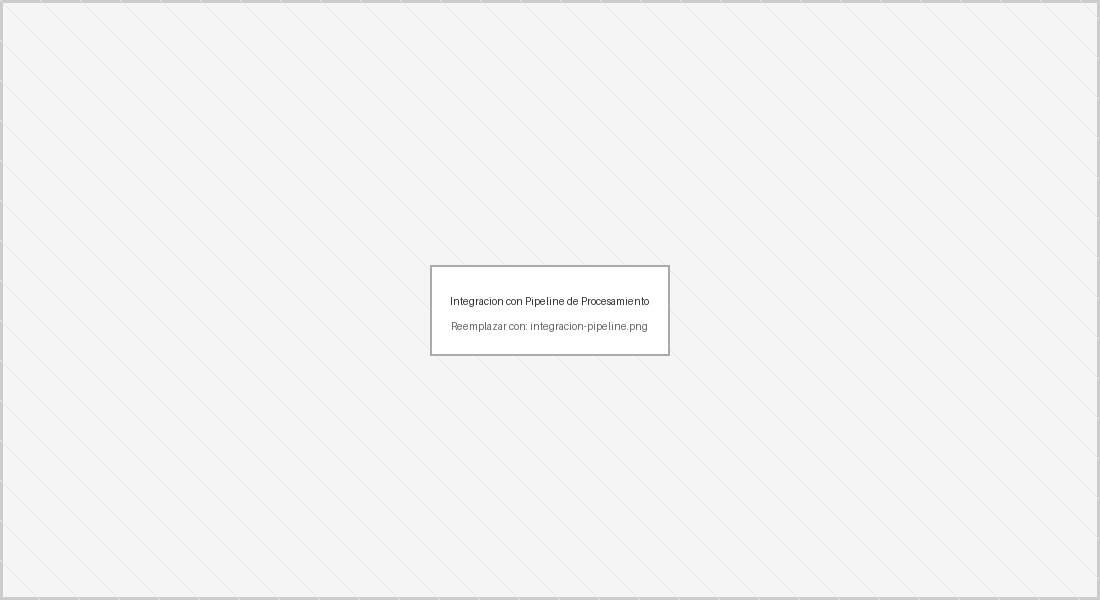
\includegraphics[width=0.9\textwidth]{images/integracion-pipeline.png}
\caption{Integración del sistema de visualización con el pipeline de procesamiento}
\label{fig:integracion-pipeline}
\end{figure}

\subsubsection{Beneficios de la arquitectura de integración}

\begin{itemize}
    \item \textbf{Desacoplamiento}: El sistema de visualización es independiente del pipeline de procesamiento, permitiendo evolucionar cada componente por separado.

    \item \textbf{Escalabilidad}: Múltiples instancias del servidor de visualización pueden conectarse a la misma base de datos sin conflictos.

    \item \textbf{Tolerancia a fallos}: Si el pipeline de procesamiento falla, el sistema de visualización continúa funcionando con los últimos datos disponibles.

    \item \textbf{Flexibilidad}: Es posible agregar nuevas fuentes de datos al pipeline sin modificar el sistema de visualización, siempre que se mantenga el esquema de las colecciones.
\end{itemize}

\subsection{Resumen de funcionalidades implementadas}\label{resumen-funcionalidades}

La Tabla \ref{tab:resumen-funcionalidades} presenta un resumen consolidado de todas las funcionalidades implementadas en el sistema de visualización y monitorización.

\begin{table}[H]
\centering
\small
\begin{tabular}{|l|p{7cm}|l|}
\hline
\textbf{Categoría} & \textbf{Funcionalidad} & \textbf{Estado} \\
\hline
\multirow{5}{*}{Visualizaciones} & Gráfico de casos por departamento & Implementado \\
& Distribución por sexo (casos y fallecidos) & Implementado \\
& Series temporales (casos y fallecidos) & Implementado \\
& Histograma de grupos de edad & Implementado \\
& Mapas de calor (casos, fallecidos, hospitalizaciones) & Implementado \\
\hline
\multirow{3}{*}{Filtros} & Filtro por departamento & Implementado \\
& Filtro por sexo & Implementado \\
& Búsqueda de departamento & Implementado \\
\hline
\multirow{4}{*}{Indicadores} & Total de casos & Implementado \\
& Casos positivos & Implementado \\
& Hospitalizaciones & Implementado \\
& Fallecidos & Implementado \\
\hline
\multirow{6}{*}{Alertas} & Alerta por total de casos & Implementado \\
& Alerta por casos positivos & Implementado \\
& Alerta por fallecidos & Implementado \\
& Alerta por hospitalizaciones & Implementado \\
& Alerta por casos por departamento & Implementado \\
& Alerta por fallecidos por departamento & Implementado \\
\hline
\multirow{4}{*}{Tiempo Real} & Actualización automática de gráficos & Implementado \\
& Notificaciones de cambios & Implementado \\
& Indicador de conexión & Implementado \\
& Propagación de alertas & Implementado \\
\hline
\end{tabular}
\caption{Resumen de funcionalidades implementadas en el sistema}
\label{tab:resumen-funcionalidades}
\end{table}

\subsection{Evaluación del sistema y resultados}\label{evaluaciuxf3n-del-sistema-y-resultados}

\subsection{Criterios y métricas de evaluación}\label{criterios-y-muxe9tricas-de-evaluaciuxf3n}

La evaluación del sistema desarrollado se realiza con el objetivo de verificar el cumplimiento de los requisitos definidos y validar la utilidad práctica de la arquitectura propuesta. Para ello, se establecen métricas cuantitativas y cualitativas que permiten analizar el rendimiento del pipeline, la precisión de los modelos analíticos y la eficacia del sistema en un contexto de análisis epidemiológico.

Las métricas consideradas se agrupan en las siguientes categorías:

\subsubsection{Métricas de rendimiento}\label{muxe9tricas-de-rendimiento}

\begin{itemize}
      \tightlist
      \item
            \textbf{Latencia end-to-end}: tiempo transcurrido desde la generación del evento hasta su disponibilidad en los sistemas de visualización.
      \item
            \textbf{Throughput}: número de eventos procesados por unidad de tiempo.
      \item
            \textbf{Uso de recursos}: consumo de CPU, memoria y almacenamiento durante la ejecución del pipeline.
\end{itemize}

\subsubsection{Métricas de calidad analítica}\label{muxe9tricas-de-calidad-analuxedtica}

\begin{itemize}
      \tightlist
      \item
            \textbf{Precisión de los modelos predictivos}: medida mediante indicadores como error medio absoluto (MAE) o raíz del error cuadrático medio (RMSE).
      \item
            \textbf{Consistencia de resultados}: comparación entre métricas obtenidas en \emph{streaming} y \emph{batch}.
\end{itemize}

\subsubsection{Métricas de robustez}\label{muxe9tricas-de-robustez}

\begin{itemize}
      \tightlist
      \item
            \textbf{Tolerancia a fallos}: capacidad del sistema para recuperarse ante interrupciones parciales.
      \item
            \textbf{Escalabilidad}: comportamiento del sistema frente a incrementos en la tasa de eventos.
\end{itemize}

\subsubsection{Métricas de utilidad práctica}\label{muxe9tricas-de-utilidad-pruxe1ctica}

\begin{itemize}
      \tightlist
      \item
            Actualización en tiempo real de dashboards.
      \item
            Capacidad de detección temprana de eventos críticos.
\end{itemize}

Interpretabilidad de los resultados por parte del usuario final.

\subsection{Escenarios de evaluación}\label{escenarios-de-evaluaciuxf3n}

La evaluación se lleva a cabo mediante diferentes escenarios controlados que permiten observar el comportamiento del sistema bajo distintas condiciones:

\begin{enumerate}

      \tightlist
      \item
            \textbf{Escenario de carga normal}: flujo constante de eventos simulados.
      \item
            \textbf{Escenario de alta carga}: incremento significativo en la tasa de eventos.
      \item
            \textbf{Escenario con eventos tardíos}: introducción de retrasos artificiales en el \emph{event time}.
      \item
            \textbf{Escenario de reprocesamiento batch}: análisis de datos históricos completos.
\end{enumerate}

Estos escenarios permiten evaluar tanto el comportamiento dinámico del sistema como su capacidad de análisis retrospectivo.

\subsection{Resultados obtenidos}\label{resultados-obtenidos}

Los resultados muestran que la arquitectura basada en el modelo Dataflow es capaz de procesar datos epidemiológicos en \emph{streaming} y \emph{batch} de manera eficiente y consistente.

En términos de rendimiento, el sistema mantiene latencias reducidas incluso bajo escenarios de alta carga, demostrando una correcta gestión del paralelismo y los recursos disponibles. El throughput se incrementa de forma proporcional al aumento de eventos, evidenciando la escalabilidad del pipeline.

Respecto a la calidad analítica, los modelos predictivos implementados presentan un nivel de precisión adecuado para el análisis de tendencias epidemiológicas, permitiendo identificar patrones relevantes y posibles escenarios futuros. Asimismo, los resultados obtenidos en \emph{streaming} y \emph{batch} muestran una alta coherencia, validando el enfoque unificado del modelo Dataflow.

\subsection{Análisis comparativo}\label{anuxe1lisis-comparativo}

La comparación entre el procesamiento en tiempo real y el reprocesamiento batch evidencia que el enfoque propuesto permite combinar inmediatez y precisión. Mientras que el \emph{streaming} proporciona información actualizada para la toma de decisiones inmediata, el procesamiento batch permite validar, corregir y enriquecer los resultados mediante el análisis histórico.

Este enfoque evita la duplicación de lógica presente en arquitecturas tradicionales y reduce la complejidad operativa del sistema.

\subsection{Discusión de resultados}\label{discusiuxf3n-de-resultados}

Los resultados obtenidos confirman que la arquitectura desarrollada cumple con los objetivos específicos planteados en el TFM. La adopción del modelo Dataflow facilita la construcción de pipelines robustos, flexibles y escalables, capaces de adaptarse a escenarios de alta variabilidad en los datos.

No obstante, se identifican ciertas limitaciones, como la dependencia de la calidad de los datos de entrada y el coste computacional asociado a escenarios de alta carga. Estas limitaciones representan oportunidades para futuras mejoras y optimizaciones.

\subsection{Validación de los objetivos específicos}\label{validaciuxf3n-de-los-objetivos-especuxedficos}

La evaluación realizada permite verificar el cumplimiento de los objetivos específicos del trabajo:

\begin{itemize}
      \tightlist
      \item
            Se validó la viabilidad de una arquitectura basada en flujos de eventos.
      \item
            Se demostró la eficacia del procesamiento unificado en \emph{streaming} y \emph{batch}.
      \item
            Se comprobó la utilidad de los modelos analíticos y predictivos.
\end{itemize}

Se confirmó la capacidad del sistema para apoyar la toma de decisiones basada en datos.

\subsection{Síntesis del impacto del sistema}\label{suxedntesis-del-impacto-del-sistema}

El sistema desarrollado demuestra que el procesamiento de datos en tiempo real, combinado con análisis histórico, constituye una herramienta valiosa para el análisis epidemiológico. La arquitectura propuesta ofrece un enfoque adaptable que puede extenderse a otros dominios donde el tiempo y la precisión son factores críticos.


\subsection{Aporte y contribución del trabajo}\label{aporte-y-contribuciuxf3n-del-trabajo}

Este capítulo presenta una síntesis del valor aportado por el trabajo, destacando su contribución técnica, el valor añadido frente a soluciones existentes y su aplicabilidad en contextos reales, particularmente en el ámbito peruano.

\subsection{Resumen de la contribución técnica}\label{resumen-de-la-contribuciuxf3n-tuxe9cnica}

Este Trabajo Fin de Máster propone y valida una arquitectura de procesamiento de datos híbrida (lotes y tiempo real) basada en el modelo Dataflow, orientada al tratamiento de datos epidemiológicos a gran escala.

Las principales contribuciones técnicas del trabajo son:

\begin{itemize}
      \tightlist
      \item
            \textbf{Diseño de una arquitectura unificada} que permite procesar datos históricos en lotes (batch) y datos en tiempo real (streaming) utilizando principios comunes, evitando la duplicación de lógica.
      \item
            \textbf{Uso de Apache Kafka como capa de ingesta desacoplada}, permitiendo la simulación de flujos en tiempo real a partir de datasets históricos.
      \item
            \textbf{Aplicación de Apache Beam como capa de abstracción}, facilitando la definición de pipelines independientes del motor de ejecución.
      \item
            \textbf{Análisis conceptual del rol de Apache Flink} como motor de procesamiento para:

            \begin{itemize}
                  \tightlist
                  \item
                        cálculo de métricas agregadas
                  \item
                        detección de picos
                  \item
                        generación de señales para alertas tempranas.
            \end{itemize}
      \item
            \textbf{Modelo de persistencia flexible}, combinando almacenamiento documental (MongoDB) para explotación analítica y visualización.
      \item
            \textbf{Separación clara de responsabilidades} entre ingesta, procesamiento, almacenamiento y visualización, alineada con buenas prácticas de ingeniería de datos.
\end{itemize}

En conjunto, el trabajo demuestra cómo construir una solución escalable, extensible y mantenible para el análisis de datos epidemiológicos.

\subsection{Valor añadido frente a soluciones existentes}\label{valor-auxf1adido-frente-a-soluciones-existentes}

Frente a soluciones tradicionales o enfoques comúnmente utilizados, el trabajo aporta los siguientes elementos diferenciales:

\begin{itemize}
      \tightlist
      \item
            \textbf{Evita la complejidad de la arquitectura Lambda}, eliminando la necesidad de mantener dos pipelines separados (batch y speed layer).
      \item
            \textbf{Uso de tecnologías open-source ampliamente adoptadas}, reduciendo dependencia de soluciones propietarias y facilitando la replicabilidad..
      \item
            \textbf{Enfoque didáctico y reproducible}, al construirse sobre un entorno local controlado que puede ser replicado con fines académicos o formativos.
      \item
            \textbf{Calidad de datos integrada en el pipeline}, permitiendo tener datos limpios normalizados validados y descartar los datos inválidos con un solo proceso.
\end{itemize}

Además, el trabajo no se limita a una implementación puntual, sino que propone un \textbf{marco conceptual reutilizable} para otros proyectos de análisis de datos en tiempo real.

\subsection{Aplicabilidad en contextos reales (Perú)}\label{aplicabilidad-en-contextos-reales-peruxfa}

La arquitectura propuesta es especialmente aplicable al contexto peruano por las siguientes razones:

\begin{itemize}
      \item
            \textbf{Adecuación a la realidad de los datos públicos}, caracterizados por:

            \begin{itemize}
                  \tightlist
                  \item
                        Heterogeneidad,
                  \item
                        Retrasos en la actualización,
                  \item
                        Necesidad de reprocesamiento histórico.
            \end{itemize}
      \item
            \textbf{Capacidad de adaptación a infraestructuras limitadas}, permitiendo despliegues progresivos (local, on-premise o cloud).
      \item
            \textbf{Soporte para análisis epidemiológico continuo}, facilitando:

            \begin{itemize}
                  \tightlist
                  \item
                        Monitoreo de tendencias,
                  \item
                        Detección temprana de picos de contagio,
                  \item
                        Apoyo a la toma de decisiones por parte de entidades públicas.
            \end{itemize}
      \item
            \textbf{Potencial reutilización institucional}, tanto en el Ministerio de Salud como en gobiernos regionales o universidades.
      \item
            \textbf{Escalabilidad futura}, permitiendo integrar nuevas fuentes de datos sin rediseñar completamente la arquitectura.
\end{itemize}

De este modo, el trabajo no solo tiene valor académico, sino que presenta una propuesta técnicamente viable y contextualizada para la realidad peruana.

\subsection{Cierre del capítulo}\label{cierre-del-capuxedtulo}

En conclusión, este Trabajo Fin de Máster aporta una solución técnica sólida, moderna y adaptable para el procesamiento y análisis de datos epidemiológicos, demostrando la viabilidad del modelo Dataflow en escenarios reales.

La combinación de fundamentos teóricos, diseño arquitectónico y análisis aplicado permite establecer una base sobre la cual pueden desarrollarse futuras extensiones, tanto en el ámbito de la investigación como en el de la gestión pública de datos.

\clearpage
\section{Código fuente y datos analizados}\label{cuxf3digo-fuente-y-datos-analizados}


\subsection{Código fuente}\label{cuxf3digo-fuente}

El código fuente desarrollado durante la realización de este Trabajo Fin de Máster ha sido implementado íntegramente por el autor y se encuentra alojado en un repositorio de control de versiones de acceso público.

El repositorio es de autoría exclusiva de los estudiantes Arthur y Gary, no existiendo contribuciones ni \emph{commits} realizados por terceros, en cumplimiento de los requisitos establecidos para este tipo de trabajos académicos.

En dicho repositorio se incluye el código correspondiente a:

\begin{itemize}
      \tightlist
      \item
            los procesos de ingesta de datos,
      \item
            los pipelines de procesamiento batch y streaming,
      \item
            los scripts de transformación y normalización,
      \item
            y los elementos necesarios para la persistencia y visualización de los datos.
\end{itemize}

La URL del repositorio es la siguiente:

\textbf{Repositorio Git:\\
} \emph{https://github.com/arthur8davis/tfm-dataflow-architecture}

\subsubsection{Datos analizados}\label{datos-analizados}

Los datos utilizados para el desarrollo y validación del trabajo proceden de fuentes públicas, concretamente de datasets relacionados con casos epidemiológicos de COVID-19 en el Perú.

Con el objetivo de garantizar la transparencia, la reproducibilidad y la trazabilidad del análisis, los datos empleados se encuentran también disponibles dentro del mismo repositorio, en formato estructurado, junto con una descripción de su origen y esquema.

Durante todo el proceso:

\begin{itemize}
      \tightlist
      \item
            los datos han sido tratados de forma anonimizada,
      \item
            no se ha manejado información que permita la identificación directa o indirecta de personas físicas,
      \item
            y se ha respetado la normativa vigente en materia de protección de datos.
\end{itemize}

\subsubsection{Consideraciones sobre confidencialidad}\label{consideraciones-sobre-confidencialidad}

Dado que este Trabajo Fin de Máster se ha desarrollado en un contexto académico y a partir de datos públicos, no existen restricciones de confidencialidad que impidan la publicación del código fuente ni de los datos utilizados.

En consecuencia, tanto el código como los datos quedan disponibles con fines académicos y de investigación, permitiendo su consulta, análisis y reutilización bajo las condiciones indicadas en el repositorio.

\clearpage
\section{Conclusiones}\label{conclusiones}

El presente Trabajo Fin de Máster ha abordado el problema del procesamiento y análisis eficiente de datos epidemiológicos en contextos donde coexisten grandes volúmenes de información histórica y la necesidad de obtener resultados con baja latencia para apoyar la toma de decisiones. Este problema se evidenció de forma clara durante la pandemia de COVID-19, especialmente en países como el Perú, donde los sistemas tradicionales de análisis se basaron mayoritariamente en enfoques \emph{batch}, limitando la capacidad de reacción ante cambios rápidos en la evolución de los contagios.

Para dar respuesta a este problema, el trabajo ha propuesto una arquitectura de procesamiento de datos basada en el modelo Dataflow, capaz de integrar de forma coherente el procesamiento en lotes y en tiempo real. La solución se ha fundamentado en tecnologías open-source ampliamente utilizadas en la ingeniería de datos moderna, como Apache Kafka, Apache Beam y Apache Flink, combinadas con un modelo de almacenamiento flexible orientado a la explotación analítica y la visualización.

La validez de la solución propuesta se sustenta en varios aspectos. En primer lugar, el modelo arquitectónico permite desacoplar la ingesta, el procesamiento y el almacenamiento, favoreciendo la escalabilidad y la mantenibilidad del sistema. En segundo lugar, la utilización de un enfoque orientado a eventos posibilita el reprocesamiento histórico y la extensión futura del sistema sin necesidad de rediseñar completamente la arquitectura. Finalmente, la solución se ha diseñado teniendo en cuenta las limitaciones y características reales de los datos disponibles en el contexto peruano, lo que refuerza su aplicabilidad práctica.

\clearpage
\section{Limitaciones y prospectiva}\label{limitaciones-y-prospectiva}

\subsection{Limitaciones}\label{limitaciones}

Una vez finalizado el trabajo, es necesario realizar una valoración crítica de la solución propuesta, identificando aquellas limitaciones que han condicionado su desarrollo y alcance.

En primer lugar, una de las principales limitaciones del trabajo está relacionada con la calidad y naturaleza de los datos disponibles. Los datasets utilizados, aun siendo de carácter público, presentan heterogeneidad en formatos, retrasos en la actualización y posibles inconsistencias, lo que ha requerido procesos de normalización y validación que pueden afectar a la precisión de ciertos análisis. Asimismo, el estudio se ha centrado en un conjunto limitado de variables, lo que impide evaluar con mayor profundidad otros factores relevantes en la evolución de la pandemia.

En segundo lugar, el trabajo se ha enfocado principalmente en el diseño y validación arquitectónica, más que en la explotación avanzada de técnicas analíticas o predictivas. Aunque se ha analizado conceptualmente la detección de picos y la generación de métricas en tiempo real, no se ha desarrollado un sistema completo de alertas automáticas ni modelos predictivos avanzados, lo que limita el alcance funcional de la solución.

Otra limitación importante es que la arquitectura ha sido validada en un entorno controlado, utilizando simulación de flujos en tiempo real a partir de datos históricos. Si bien este enfoque es adecuado para fines académicos, un despliegue en producción requeriría pruebas adicionales de rendimiento, tolerancia a fallos y escalabilidad bajo cargas reales.

Finalmente, el trabajo no aborda de forma exhaustiva aspectos organizativos y de gobernanza de datos, como la integración con sistemas institucionales existentes, la definición de roles operativos o los procesos formales de mantenimiento y evolución de la plataforma.

\subsection{Trabajo Futuro}\label{trabajo-futuro}

A partir de las limitaciones identificadas, se abren diversas líneas de trabajo futuro que permitirían ampliar y enriquecer la aportación realizada.

En primer lugar, una extensión natural del trabajo consistiría en la incorporación de nuevas fuentes y variables, tales como datos de hospitalización, ocupación de UCI, vacunación o movilidad poblacional, lo que permitiría obtener una visión más completa del fenómeno epidemiológico.

En segundo lugar, se podría avanzar hacia la implementación efectiva de mecanismos de detección de eventos relevantes, como picos de contagio o anomalías, mediante el uso de ventanas temporales, técnicas estadísticas o modelos de aprendizaje automático integrados en motores de procesamiento en tiempo real como Apache Flink.

Otra línea de trabajo relevante sería la evolución hacia un despliegue productivo, incorporando mecanismos de monitorización, tolerancia a fallos, balanceo de carga y escalado automático, así como la evaluación comparativa del rendimiento en distintos entornos (on-premise y cloud).

Asimismo, la arquitectura propuesta podría adaptarse a otros dominios más allá del ámbito epidemiológico, como la gestión de emergencias, el análisis de movilidad urbana o el monitoreo de servicios públicos, demostrando su carácter generalizable.

Por último, futuras investigaciones podrían centrarse en aspectos de gobernanza y calidad del dato, incluyendo políticas de versionado, trazabilidad, auditoría y cumplimiento normativo, especialmente relevantes en sistemas de análisis de datos a gran escala.

\newpage
\section*{Referencias bibliograficas}
\addcontentsline{toc}{section}{Referencias bibliograficas}
\printbibliography[heading=none]

\newpage
\section*{Anexo A. Privacidad y protección de datos}
\addcontentsline{toc}{section}{Anexo A. Privacidad y protección de datos}
El presente anexo establece las directrices a seguir por el alumno en la
elaboración de su memoria, cuando requiera cumplir con la normativa de
privacidad y protección de datos personales. (\textbf{ver
      instrucciones})
\end{document}
